\chapter{Hazerd: an outdoor scene dataset and benchmark for Single image dehazing}
\label{cha3}
\chaptermark{Hazerd: a dehazing dataset and benchmark}

\section{Introduction}
\label{sec:3.1.intro}
Haze is a common degradation encountered in outdoor images, where image contrast is reduced due to light scattered by particles suspended in the air. Koschmieder~\cite{Koschmieder24,McCartney76} proposed a classical physical model to explain haze, in which horizontal airlight from scattering and light reflected by objects, transmitted and attenuated in the propagation through the hazy air, both contribute to the final images and the ratio of their contributions are controlled by the optical thickness of the media between the camera sensor and the object being imaged. The loss of detail caused by haze makes images aesthetically unappealing and also poses challenges for both human and machine vision, making it difficult to recognize and track objects and to navigate.

To mitigate the impact of haze, physics-based algorithms have been proposed for haze removal or {\em dehazing}. Early works mainly focus on image dehazing utilizing additional information. Such works includes: in~\cite{narasimhan2003contrast}, two images under different weather conditions for the same location are exploited for haze removal; in~\cite{kopf2008deep}, rough geological information is used; and in~\cite{schaul2009color}, the fusion  of near-infrared images and the hazy images are utilized for enhancing the details. These algorithms need multiple images or additional information. Though proved to be efficient, these works need either multiple images or information other than RGB images, which may be inaccessible for general applications, for example outdoor image dehazing taken by mainstream consumer-level digital cameras.

In this chapter we focus on single image dehazing methods that typically seek to estimate both the airlight and the transmission from a single hazy image, which is an ill-posed problem. To address the ill-posedness most algorithms impose additional constraints or assumptions to obtain solutions. In~\cite{fattal2008single,fattal2014dehazing,berman2016non}, color-line or haze-line has been used for modeling the spatial variance of similar color objects. In~\cite{tarel2009fast}, constraints on air veil are imposed based on the physical model. In~\cite{tan2008visibility}, the assumption of higher contrast and local smoothness are introduced. In~\cite{he2011single}, a dark channel prior is proposed that postulates that the color channel with lowest intensity represents airlight. The dark prior is extended in~\cite{meng2013efficient} to accommodate color boundary constraints. An alternative color attenuation prior is used with supervised learning in~\cite{zhu2015fast} and image fusion based approaches are proposed in~\cite{ancuti2010fast,ancuti2013single}.
In~\cite{nishino2012bayesian}, a Bayesian framework for haze estimation is described. In~\cite{cai2016dehazenet, Ren-ECCV-2016}, deep learning networks are designed for estimating the transmission map.

Despite the large number of algorithms proposed for single image dehazing, there are no established criteria or metrics for their evaluation and past publications have primarily relied on subjective comparisons on a limited number of images, with different publications using different sets of images. Three datasets: FRIDA~\cite{tarel2012vision}, D-hazy~\cite{7532754}, and CHIC~\cite{el2016color} have been proposed in prior work for objective evaluation of algorithms. FRIDA~\cite{tarel2012vision} is rather specialized and provides several synthetic hazy road images from a driver's viewpoint. D-hazy uses depth images from the Middlebury~\cite{scharstein2014high} and the NYU depth V2~\cite{silberman2012indoor} which are indoor scenes not representative of the typical dehazing applications. CHIC uses a fog machine in an indoor environment and provides 2 indoor scenes with known objects (e.g. Macbeth color checker) and 2 scenes that include outdoor content seen through windows. The indoor fog generation makes these images atypical, particularly for the case where an outdoor haze-free scene is seen from haze within the room.

In this
chapter, we provide a new image dataset {\em HazeRD}, {\em Haze Realistic Dataset}, for benchmarking of dehazing algorithms that consists of ten different actual outdoor scenes at high resolution with simulated haze under five different weather conditions, where realistic parameter values are chosen based on scattering theory. As compared to the indoor scenes used in~\cite{7532754}, these scenes are more representative of the outdoor conditions under which dehazing is of interest and they correspond to actual images as opposed to the synthetically generated versions in~\cite{tarel2012vision}. We benchmark a number of single image dehazing algorithms both on the proposed new dataset and on the existing D-hazy dataset~\cite{7532754}. Our results demonstrate that there are significant differences between the performance of the different algorithms on different datasets and the rank order of algorithms is by no means constant over the different datasets, thereby emphasizing the need for datasets like ours that are matched with realistic conditions under which dehazing is utilized.

The chapter is organized as follows. Section~\ref{sec:3.2.model} discusses the physical model for atmosphere scattering and image formation; Section~\ref{sec:3.3.simu} describes the simulation process; Section~\ref{sec:3.4.dataset} discusses the HazeRD dataset; Section~\ref{sec:3.5.benchmark} briefly summarizes some state of art dehazing techniques and their performance; at last, Section~\ref{sec:3.6.discussion}, discusses some noteworthy points about dehazing problems and the future work that may be done with HazeRD.

\section{physical model for haze}
\label{sec:3.2.model}
Atmospheric optics interprets the propagation of light in haze or fog as the process of light random diffusion and reflection by the particles in the air. Hazy weather is caused by the particles, mainly water droplets distributed in the air, which vary in both the size and the density. Haze, fog and cloud in principle share the same components, namely the air with multiple sized water droplets, but differ in the average size and distribution. The scattering of single water droplet has different behaviours regarding to the size, or the radius of the droplet: Rayleigh scattering deals with conditions that the radius is of the size of visible light wavelengths, which corresponding to almost clear weather; and Mie scattering deals with those with the radius far beyond the wavelengths, which displays high anisotrophy in the scattered light. The accumulated contribution of the distribution of the water droplets ultimately form the scattered light of the incident light. Table~\ref{table:hazelvl} lists different weather and the corresponding particles making the main contribution.
\begin{figure}[t]
\centering
\centerline{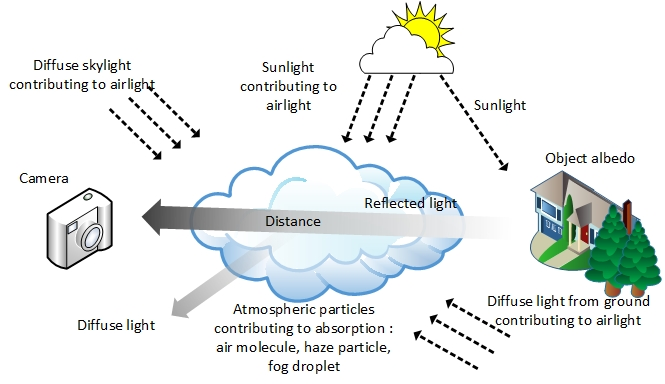
\includegraphics[width=0.95\columnwidth]{hazerd/physical_model.jpg}}
\caption{The physical model for haze. Light at the sensor is composed of airlight scattered by particles suspended in the air and light reflected from imaged objects, which is attenuated when propagating through the air.}
\label{fig:3.2.physical}
\end{figure}

\begin{table}[t]
\centering
\resizebox{0.8\textwidth}{!}{\begin{tabular}{l|l|l}
Type           & Radius($\mu m$)                                    & Concentration($cm^-3$)          \\\hline
Air molecule   & $10^{-4}$ & $10^{19}$ \\
Aitken nucleus & $10^{-4}$-$10^{-2}$ & $10^4$-$10^2$       \\
Haze Particle  & $10^{-2}$-$1$                     & $10^2$-$1$ \\
Fog droplet    & 1-10                                          & 100-10                                          \\
Cloud droplet  & 1-10                                          & 300-10                                          \\
Raindrop       & $10^2$-$10^4$     & $10^{-2}$-$10^{-5}$
\end{tabular}}
\caption{Particle sizes for different weather}
\label{table:hazelvl}
\end{table}

As refer to above, Mie scattering theory~\cite[Chap. 5, 6]{McCartney76}, which applies when particle sizes are significantly larger that the wavelengths of light involved, can be used to analyze light propagation under hazy conditions. While the exact details of Mie theory are quite involved, image formation under hazy weather can be modeled by taking two main factors into account: the airlight and the attenuation. The physical scenario is depicted in Fig.~\ref{fig:3.2.physical}. Due to the scattering of light by the particles in the haze, light from objects attenuates as it propagates from the object to the camera with an intensity that declines exponentially with distance. At the same time, part of the ambient illumination is scattered by the haze particles into the camera as {\em airlight} that increases the intensity of the image.  Assuming a homogeneous haze and a uniform ambient illumination, the spectral irradiance incident on the camera sensor plane from an object with spatially uniform spectral irradiance $E_{\lambda}$  can be written as~\cite{Koschmieder24},
\begin{equation}
I_{\lambda} = t_{\lambda} E_{\lambda} + (1-t_{\lambda})A_{\lambda},
\label{eq:3.1}
\end{equation}
where $\lambda$ denotes the wavelength,  $A_{\lambda}$ is the {\em airlight}, and $t_{\lambda} = e^{-d \beta{_\lambda}}$ is the so called {\em transmission}, with $\beta{_\lambda}$  denoting the scattering coefficient for the haze particles, and $d$ denoting the distance between the object and the camera. The product $d \beta{_\lambda}$ is called the {\em optical thickness}. Observe that as the distance $d$ increases, the contribution of airlight increases while the light from the object diminishes, leading to reduced contrast. The image captured by a typical three channel RGB (red-green-blue) camera can then be expressed as,
\begin{equation}
% \begin{aligned}
% I_{C} &= \int_{\lambda}{I_{\lambda}*R_{\lambda,C}}d\lambda \\
%  &= \int_{\lambda}{t_{\lambda}*E_{\lambda}*R_{\lambda,C}+(1-t_{\lambda})*A_{\lambda}*R_{\lambda,C}}d\lambda,
% \end{aligned}
I_{C} = \int_{\lambda}{t_{\lambda} E_{\lambda} R_{\lambda,C}+(1-t_{\lambda}) A_{\lambda} R_{\lambda,C}}d\lambda,
\label{eq:3.2}
\end{equation} 
where $C\in{\{R,G,B\}}$ represents the image channel and $R_{\lambda,C}$ the camera spectral response of the channel.

\section{Haze simulation}
\label{sec:3.3.simu}
In dense haze or fog, the scattering coefficient $\beta_{\lambda}$ is almost constant over the visible spectral region, and therefore we can simplify~\eqref{eq:3.2} by setting $\beta_{\lambda} = \beta$ for all wavelengths $\lambda$. The captured image channel intensities can then be represented as 
% Following the idea in~\cite{blasinski2013per}, in which the value of each channel is dealt with separately and pixel-wise, the relation for hazy image simulation in position $(x,y)$ is,
\begin{equation}
I_{C}(x,y) = E_{C}(x,y) t(x,y) +A_{C}(x,y) (1-t(x,y)),
\label{eq:3.3}
\end{equation}
\begin{equation*}
t(x,y) = e^{-\beta d(x,y)},
\end{equation*}
% \vspace*{-0.06in}
% \begin{align*}
% E_{C}(x,y) &= \int_{\lambda}{E_{\lambda}(x,y) R_{\lambda,C}}d\lambda,\\
% A_{C} &= \int_{\lambda}{A_{\lambda}R_{\lambda,C}}d\lambda,
% \vspace*{-0.05in}
% &\end{align*}
where $(x,y)$ denotes spatial location, 
%$E_{C}(x,y) = \int_{\lambda}{E_{\lambda}(x,y) R_{\lambda,C}}d\lambda$
\[
E_{C}(x,y) = \int_{\lambda}{E_{\lambda}(x,y) R_{\lambda,C}}d\lambda,
\]
is the irradiance of the object received by camera sensor in the absence of haze, i.e., the haze-free image, and $A_{C} = \int_{\lambda}{A_{\lambda}R_{\lambda,C}}d\lambda$ is the airlight, and the depth $d(x,y)$ denotes the distance of the object imaged at $(x,y)$ from the camera plane. Note that a key advantage of the simplified model is that hazy images can be simulated using only haze free images along with depth information using the scattering parameter $\beta$ and the airlight $A_{C}$ and the spectral distributions on the right hand side of~\eqref{eq:3.2}, which are invariably unavailable, are not required for the haze simulation. The color and gamma correction~\cite{GSharma:crcdcihbk02} in encoding the raw camera sensor values into digital images, however, need to be accounted for. Images are typically encoded in the 
sRGB color space~\cite{international1999multimedia}. We assume that the color correction matrix is absorbed into the channel sensitivities in~\eqref{eq:3.2} and the "linear" intensity values from~\eqref{eq:3.3} are nonlinearly encoded into the digital image values via the transform specified in the sRGB standard~\cite{international1999multimedia}, viz.,
\begin{equation}
C = \begin{cases}
12.92C_{L} &\text{C $\le$ 0.0031308},\\
1.055C_{L}^{1/2.4}-0.055 &\text{C $>$ 0.0031308},
\end{cases}
\label{eq:3.srgb2rgb}
\end{equation}
here $C_{L}$ is the linear RGB value for each channel, $C$ is the corresponding sRGB encoded value, where the transformation is specified on a $[0-1]$ range which is then mapped to the 8-bit digital encoding. For the simulation, the inverse of the transformation in~\eqref{eq:3.srgb2rgb} is applied to the recorded haze free image after mapping the data into the  $[0-1]$ range and once the simulated hazy images are obtained via~\eqref{eq:3.3} the transformation in~\eqref{eq:3.srgb2rgb} is applied and the images are re-encoded as 8-bit representations.

%We use visual range to describe the weather condition. 
The scattering parameter $\beta$ depends on the weather conditions. Its value is specified in terms of the intuitive notion of visual range~\cite[pp. 42]{McCartney76}, which is defined, under daylight conditions, as the distance at which the apparent contrast between a dark object and the horizon sky becomes equal to the just noticeable contrast threshold $\epsilon$ for an observer (usually set to 0.02). Specifically, the scattering parameter is obtained from the visible range $R_{m}$ via the relation $\beta = -\ln(\epsilon)/R_m $. HazeRD simulates five different conditions from light to dense fog, for which the visible range and the scattering parameter are listed in Table.~\ref{table:3.coefficient}. For simulating hazy images, HazeRD uses~\eqref{eq:3.3} with these parameter values along with captured haze free images that also have an associated depth map $d(x,y)$ available. Fig.~\ref{fig:3.simu} summarizes the the haze simulation process.

% \vspace*{-0.1in}
% \begin{equation}
% \beta = \frac{1}{R{_m}}\ln\frac{1}{\epsilon},
% \label{eq:4}
% \vspace*{-0.05in}
% \end{equation}
\begin{table}[htp]
\centering
\resizebox{0.95\textwidth}{!}{\begin{tabular}{|c|c|c|c|c|c|c|} \hline
 & 50m & 100m & 200m & 500m & 1000m \\ \hline
weather condition & dense & thick & thick & moderate & light \\ \hline
scattering coef. $\beta$ & 78.2 & 39.1 & 19.6 & 7.82 & 3.91  \\ \hline
\end{tabular}}
\caption{The visual range in HazeRD, and the corresponding weather condition and the scattering coefficient $\beta$.}
\label{table:3.coefficient}
\end{table}
\begin{figure}
\centering
\centerline{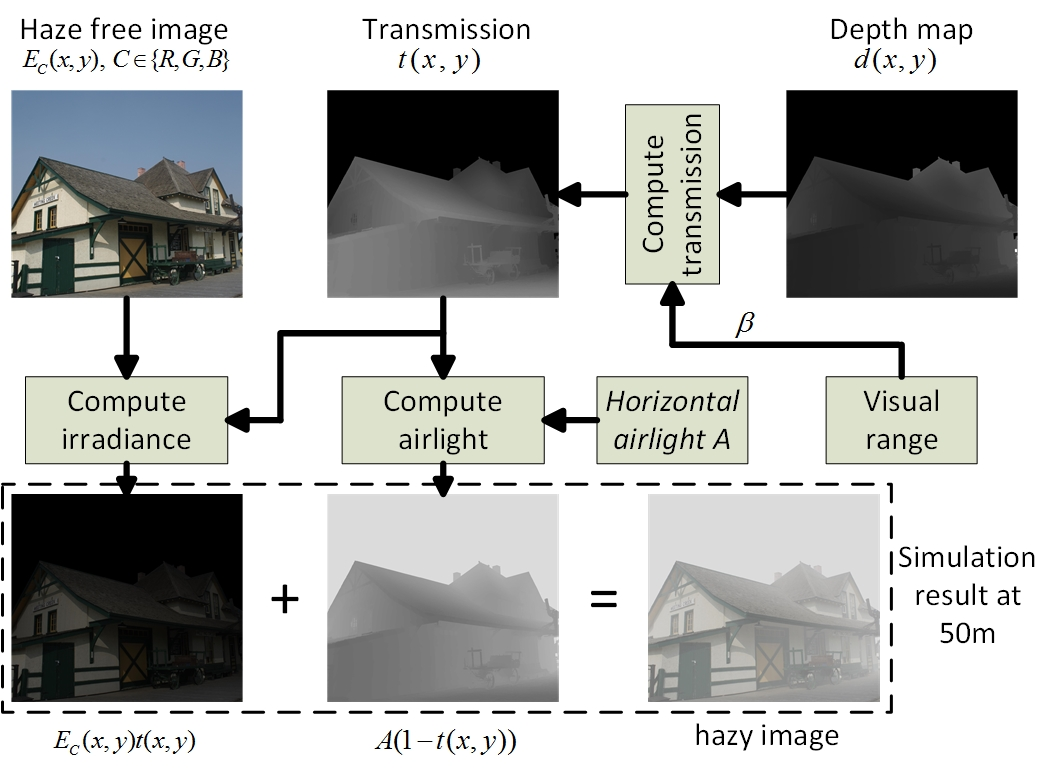
\includegraphics[width = 0.95\linewidth]{hazerd/simulation}}
\caption{Flow for haze simulation based on~\eqref{eq:3.3}.}
% TBD: Yanfu, please move the E_c(x,y) to clearly indicate that that is in the linear space
\label{fig:3.simu}
\end{figure}

% As mentioned before, the relation only holds true for visible light. In the infrared waveband, the scattering coefficient may not be viewed as constant. For example, at the wavelength of 3.61um with the visual range of 3.55km, the transmission is still as high as 0.72, whereas in the visible waveband it is only 0.1~\cite{McCartney76}. This indicates the potential of exploiting the infrared information in image dehazing or enhancement.
\section{dataset}
\label{sec:3.4.dataset}
For performance of single image dehazing algorithms, HazeRD provides ten scenes, each one having a clean RGB image and a ground truth depth map. The dataset is derived from the architectural biometrics project~\cite{Ding:ArchBio:ICIP16,ArchBioProjWebsite}, on which we first estimate the dense depth maps for each scene by fusing structure from motion and lidar~\cite{Ding:FuseLidarSFM:ICASSP17}. Five different weather conditions are simulated in each scene, ranging from light fog to dense fog, in order to test the robustness of dehazing algorithms. See Fig.~\ref{fig:3.block_diagram} for the dataset generation and benchmark block diagram. The simulation of haze and fog is performed by inverse application of ~\eqref{eq:3.srgb2rgb} followed by ~\eqref{eq:3.3}, re-white balance and redo the gamma correction. The color image values are converted to $[0,1]$ for implementing the color space transferring. Then, we use a weighted median filter~\cite{ma2013constant} and the triangular interpolation for the refinement of the depth map. The airlight is set to 0.86, to ensure a visual vividness of objects in overcast weather. Sky area, where typically depth values are missing, is set to have the distance of two times the visual range, which ensures that the transmission is of the order $10^{-4}$ and that almost no noise is introduced for normal pictures. A sample of hazy images derived from one of the original images in HazeRD is shown in Fig.~\ref{fig:3.example_dataset} for a number of different visual ranges. Figure.~\ref{fig:3.hist_compare} shows the depth histograms of HazeRD and for the Middlebury and NYU datasets that also provide images and depth maps required for haze simulation. Compared to the other two datasets which focus primarily on indoor images, the outdoor images in HazeRD span a much larger range of distance ranges and show clear clustering of different object depths. For each scene and the weather condition, a noisy version is provided. Considering the complexity of the real environment, strictly homogeneity is impossible. In atmospheric optics the main component of random fluctuations usually can be expressed by low-order Seidel aberration; here we use the Perlin noise to simulate this phenomenon~\cite{tarel2012vision}. 
\begin{figure}[htb]
% \setlength{\textfloatsep} {0pt plus 2pt minus 2pt}
% \setlength\abovecaptionskip{0pt}
% \setlength\belowcaptionskip{0pt}
\centering
\centerline{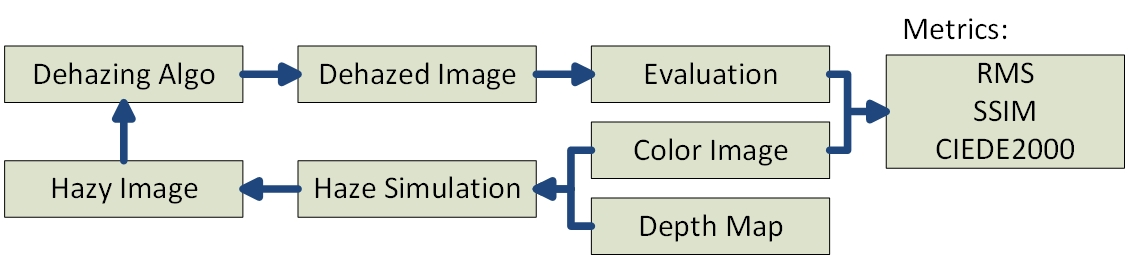
\includegraphics[width = 0.95\textwidth]{hazerd/block_diagram}}
\caption{Benchmarking workflow for evaluating dehazing algorithms using the HazeRD(proposed) and D-Hazy~\cite{7532754} dataset.}
\label{fig:3.block_diagram}
\end{figure}
\begin{figure}[htb]
\begin{minipage}[b]{0.24\linewidth}
  \centering
  \centerline{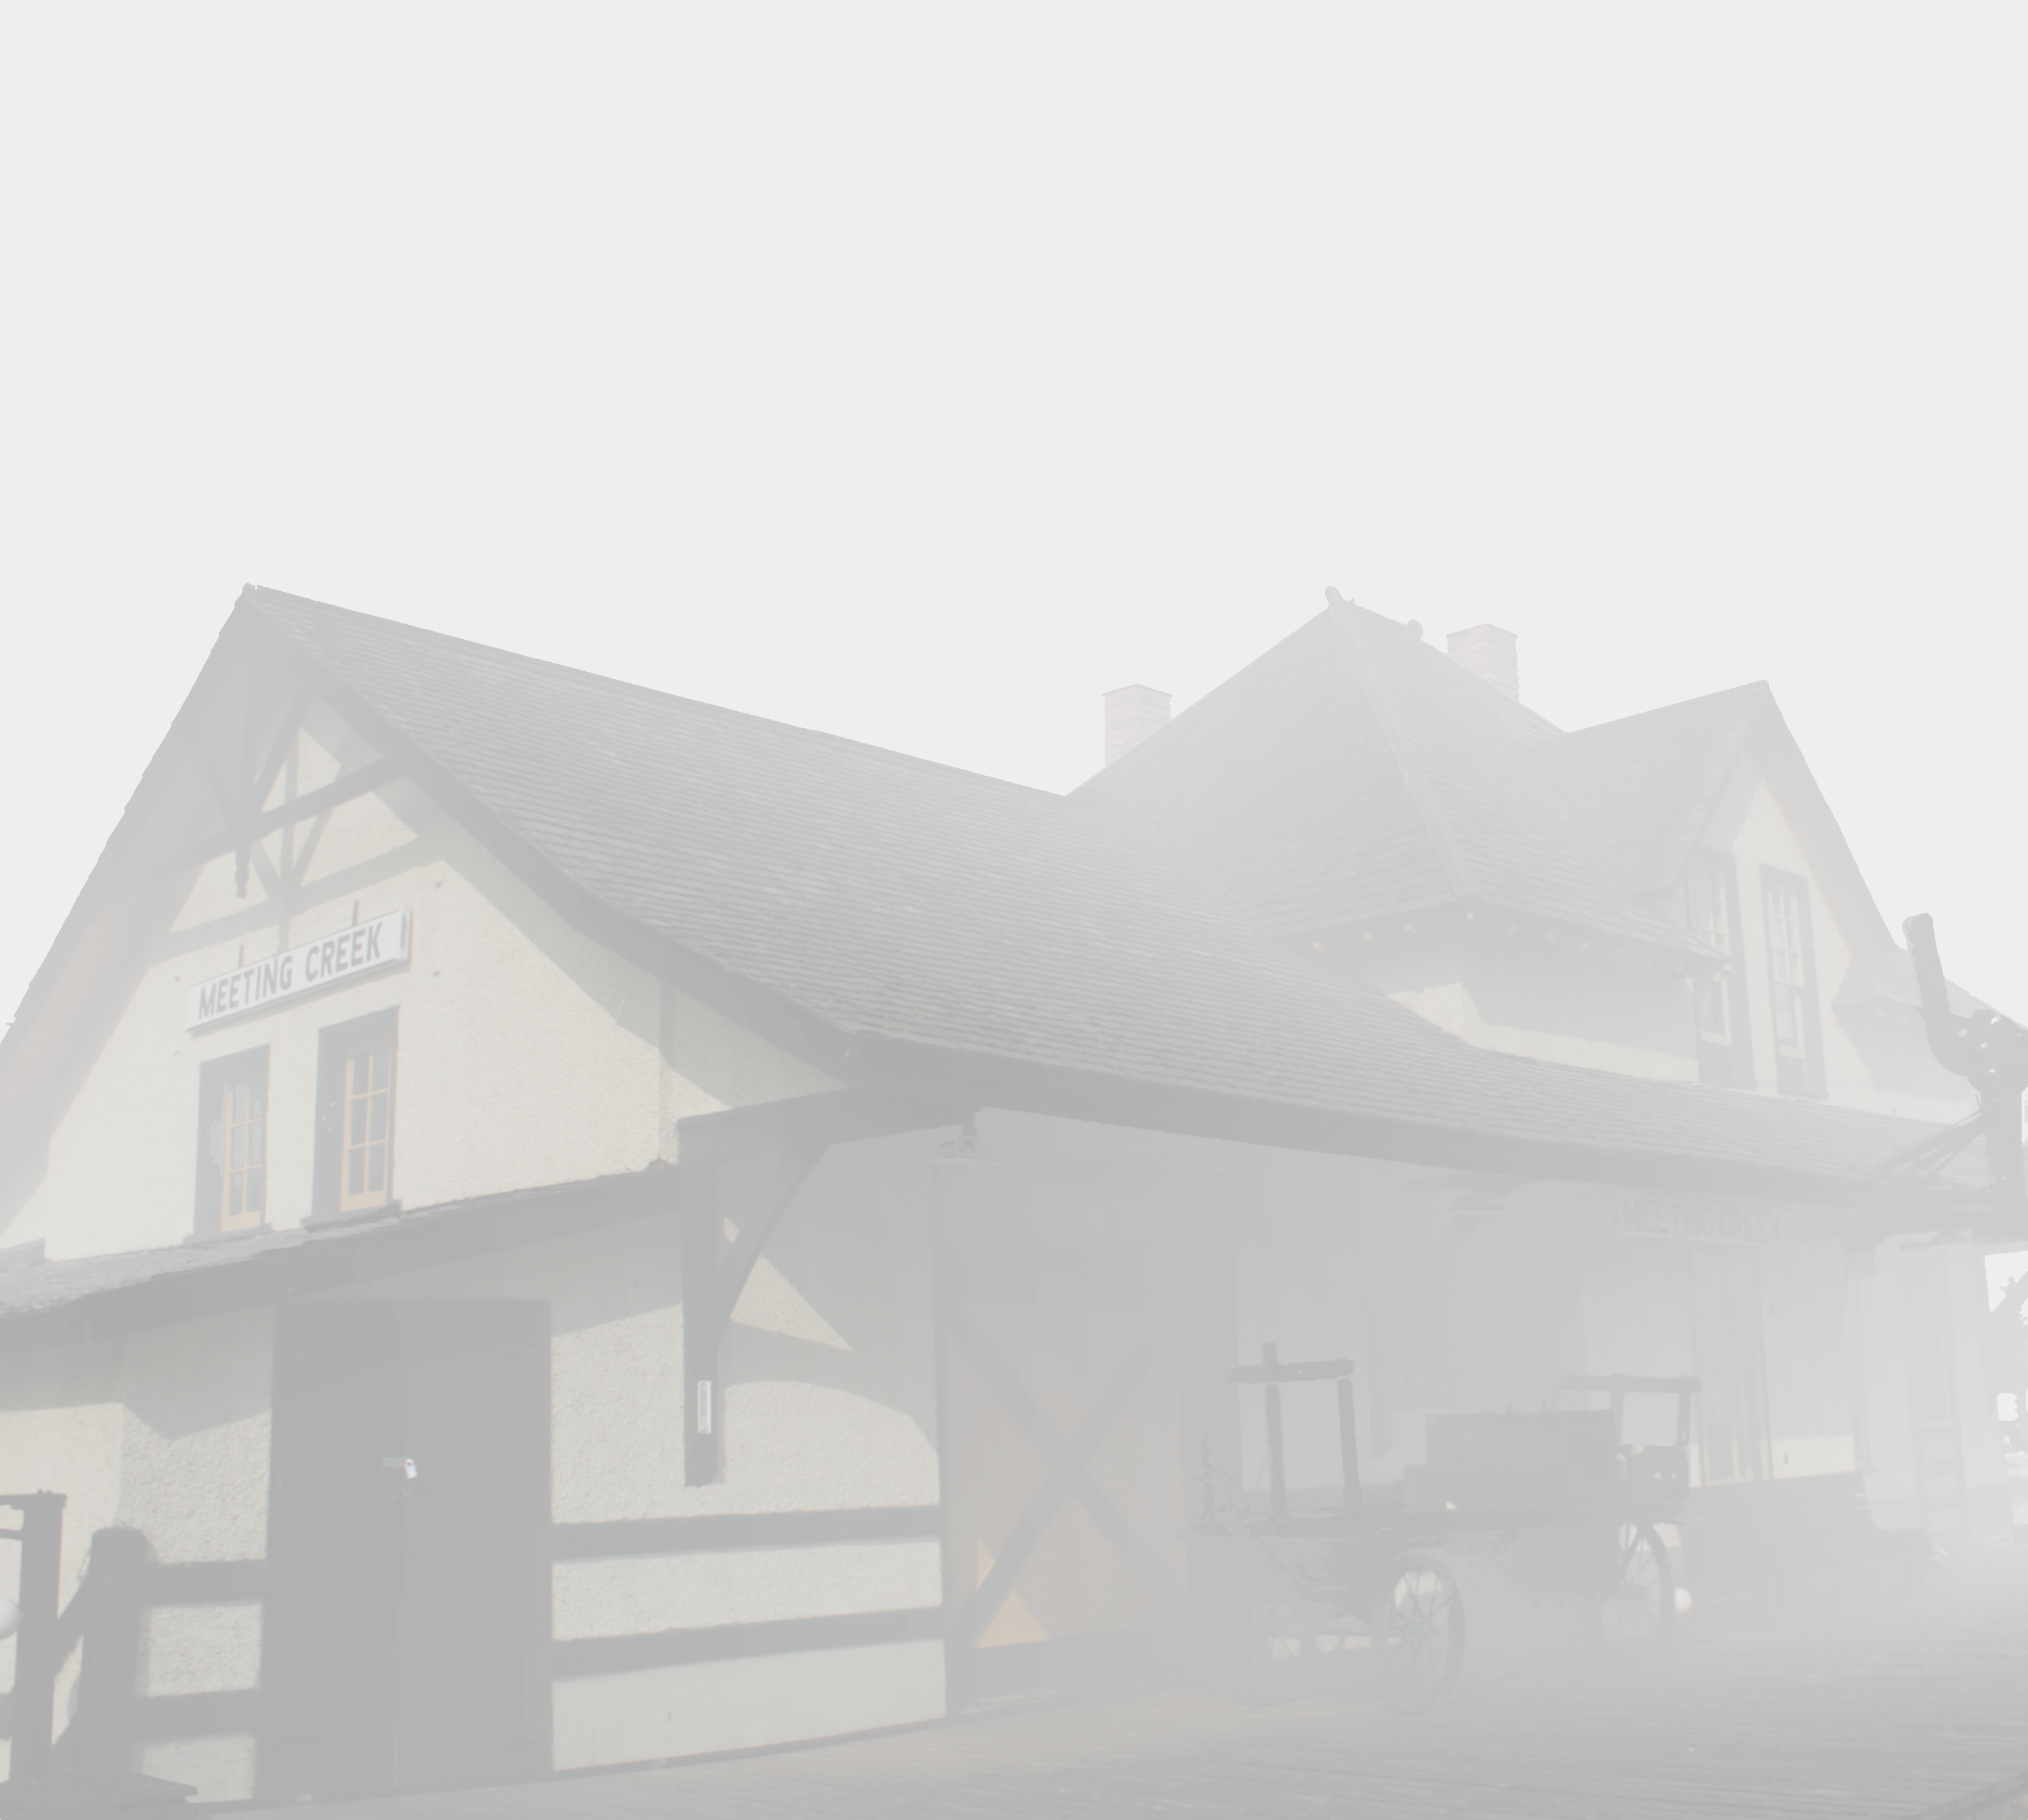
\includegraphics[width=3.2cm]{hazerd/dataset/IMG_8612_50}}
%  \vspace{1.5cm}
%   \centerline{(a)}\medskip
\end{minipage}
%
\hfill
\begin{minipage}[b]{0.24\linewidth}
  \centering
  \centerline{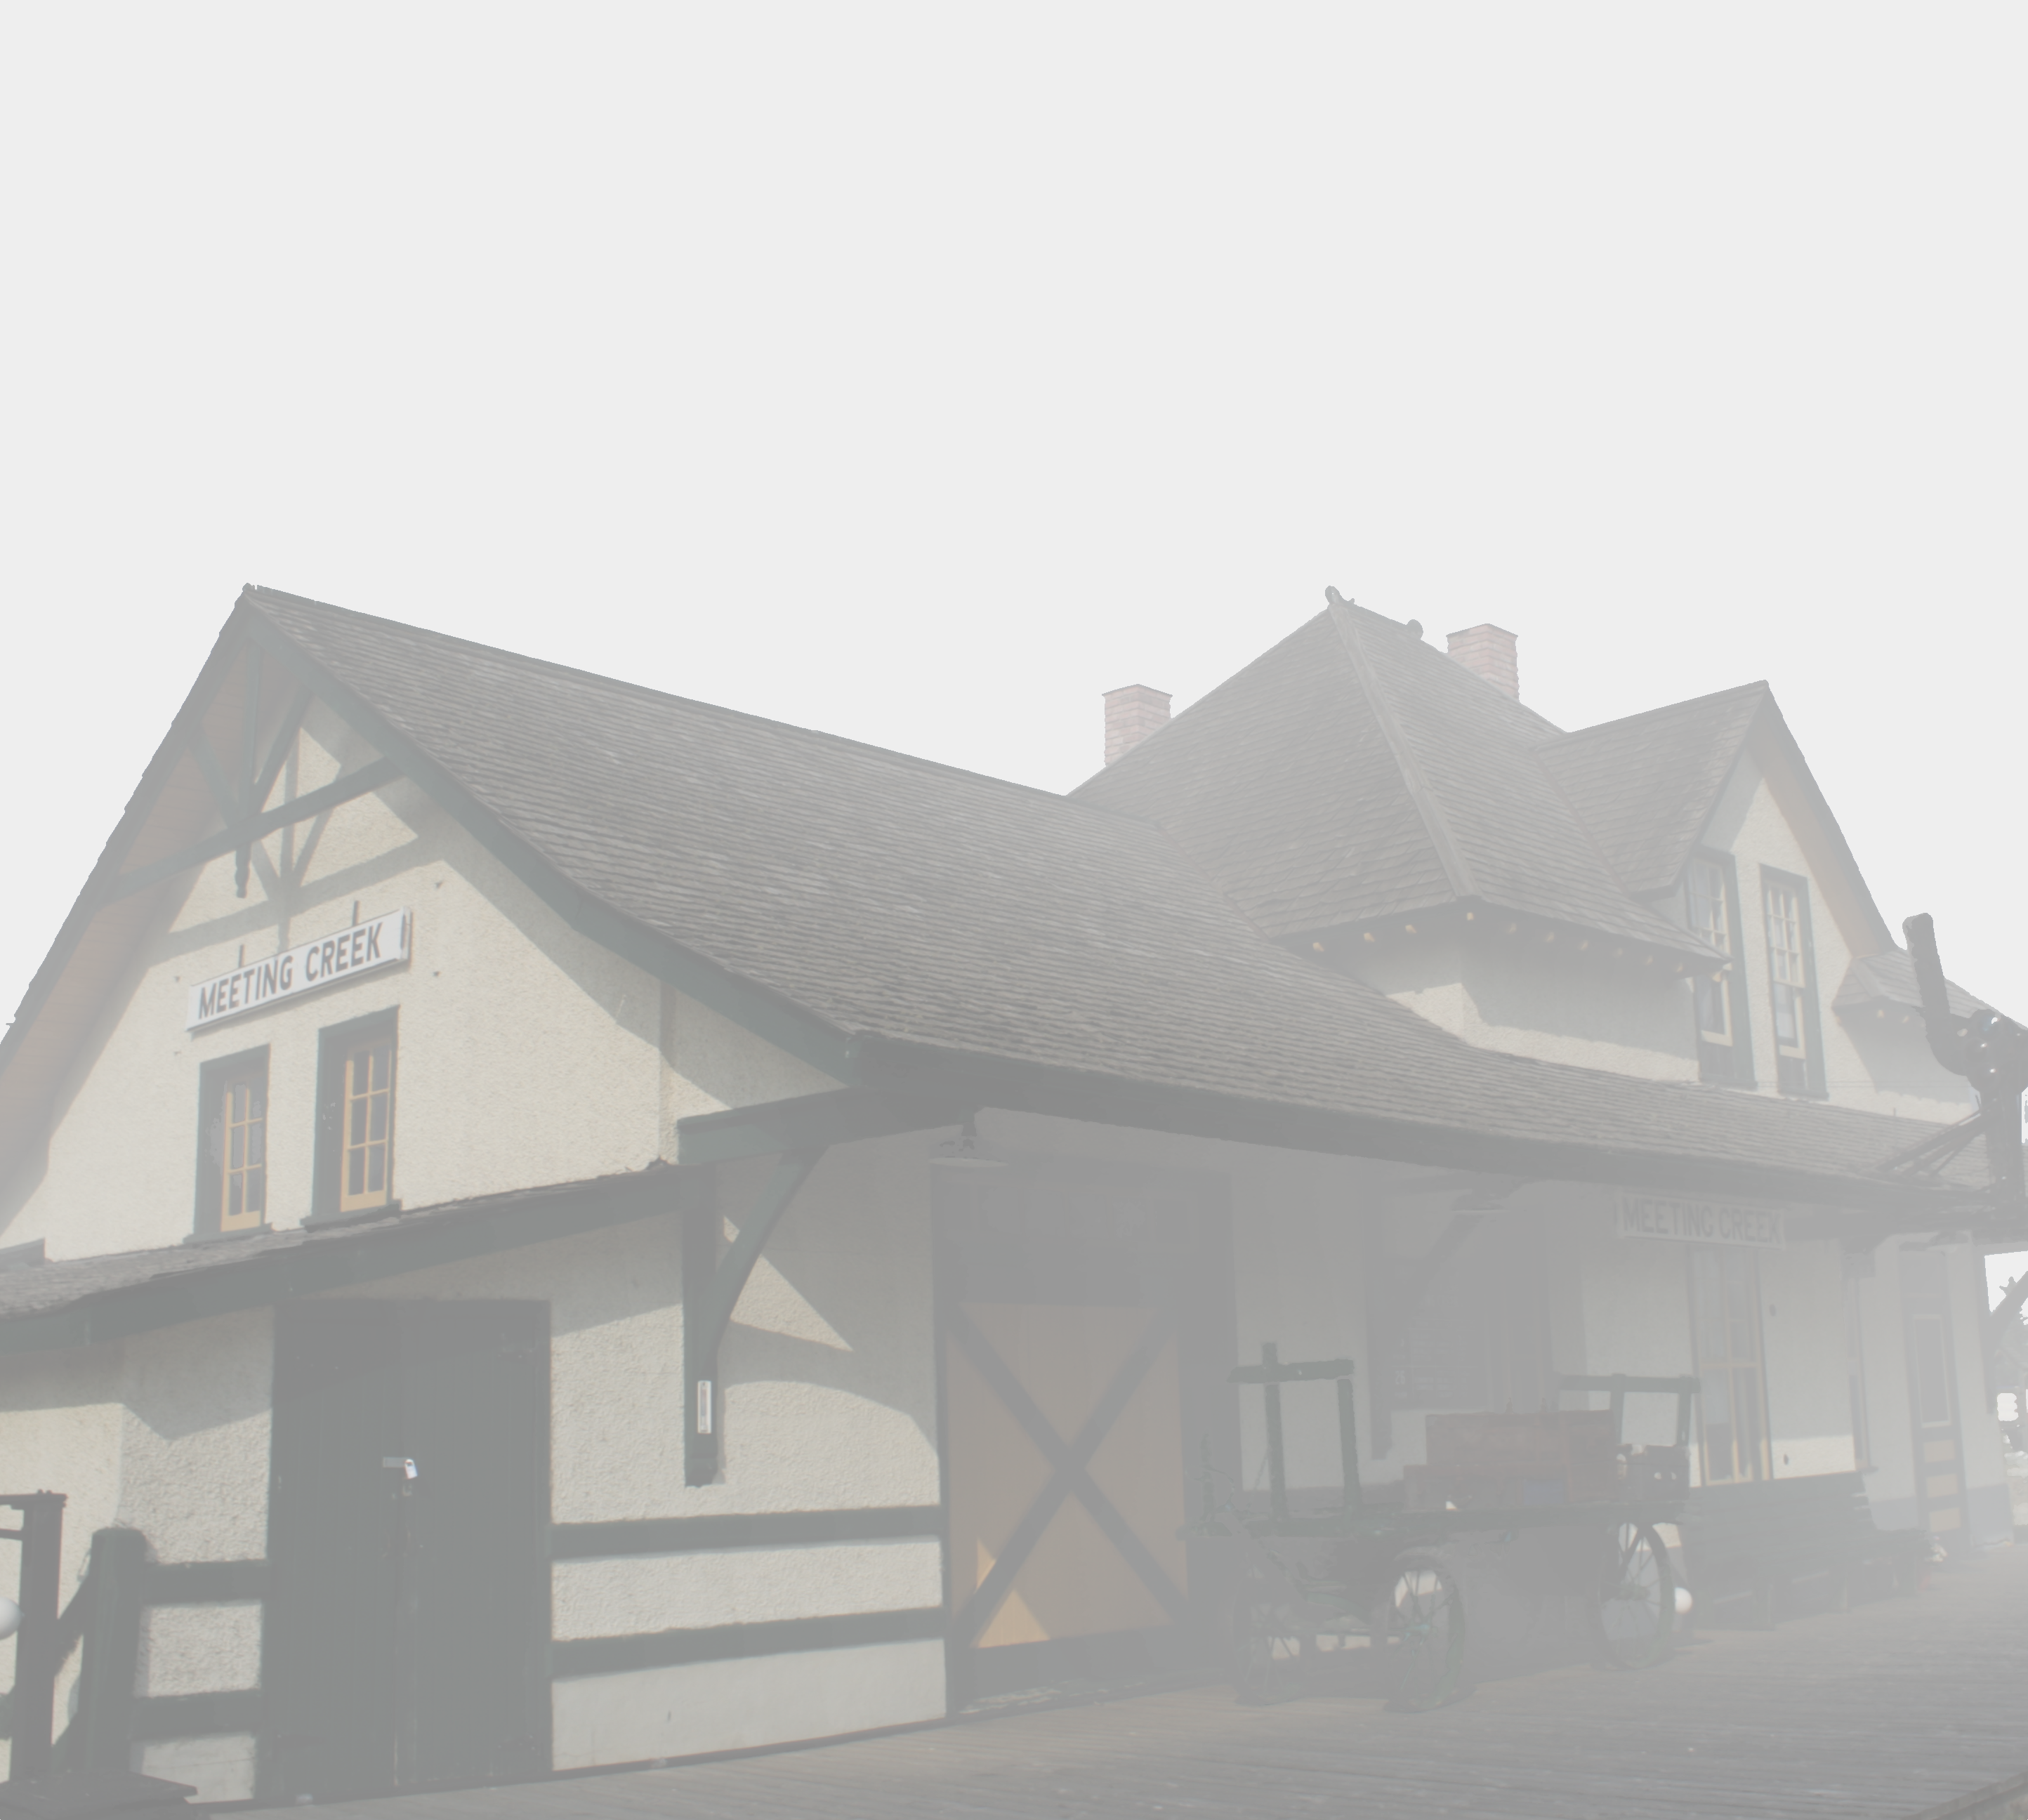
\includegraphics[width=3.2cm]{hazerd/dataset/IMG_8612_100}}
%  \vspace{1.5cm}
%   \centerline{(b)}\medskip
\end{minipage}
\hfill
\begin{minipage}[b]{0.24\linewidth}
  \centering
  \centerline{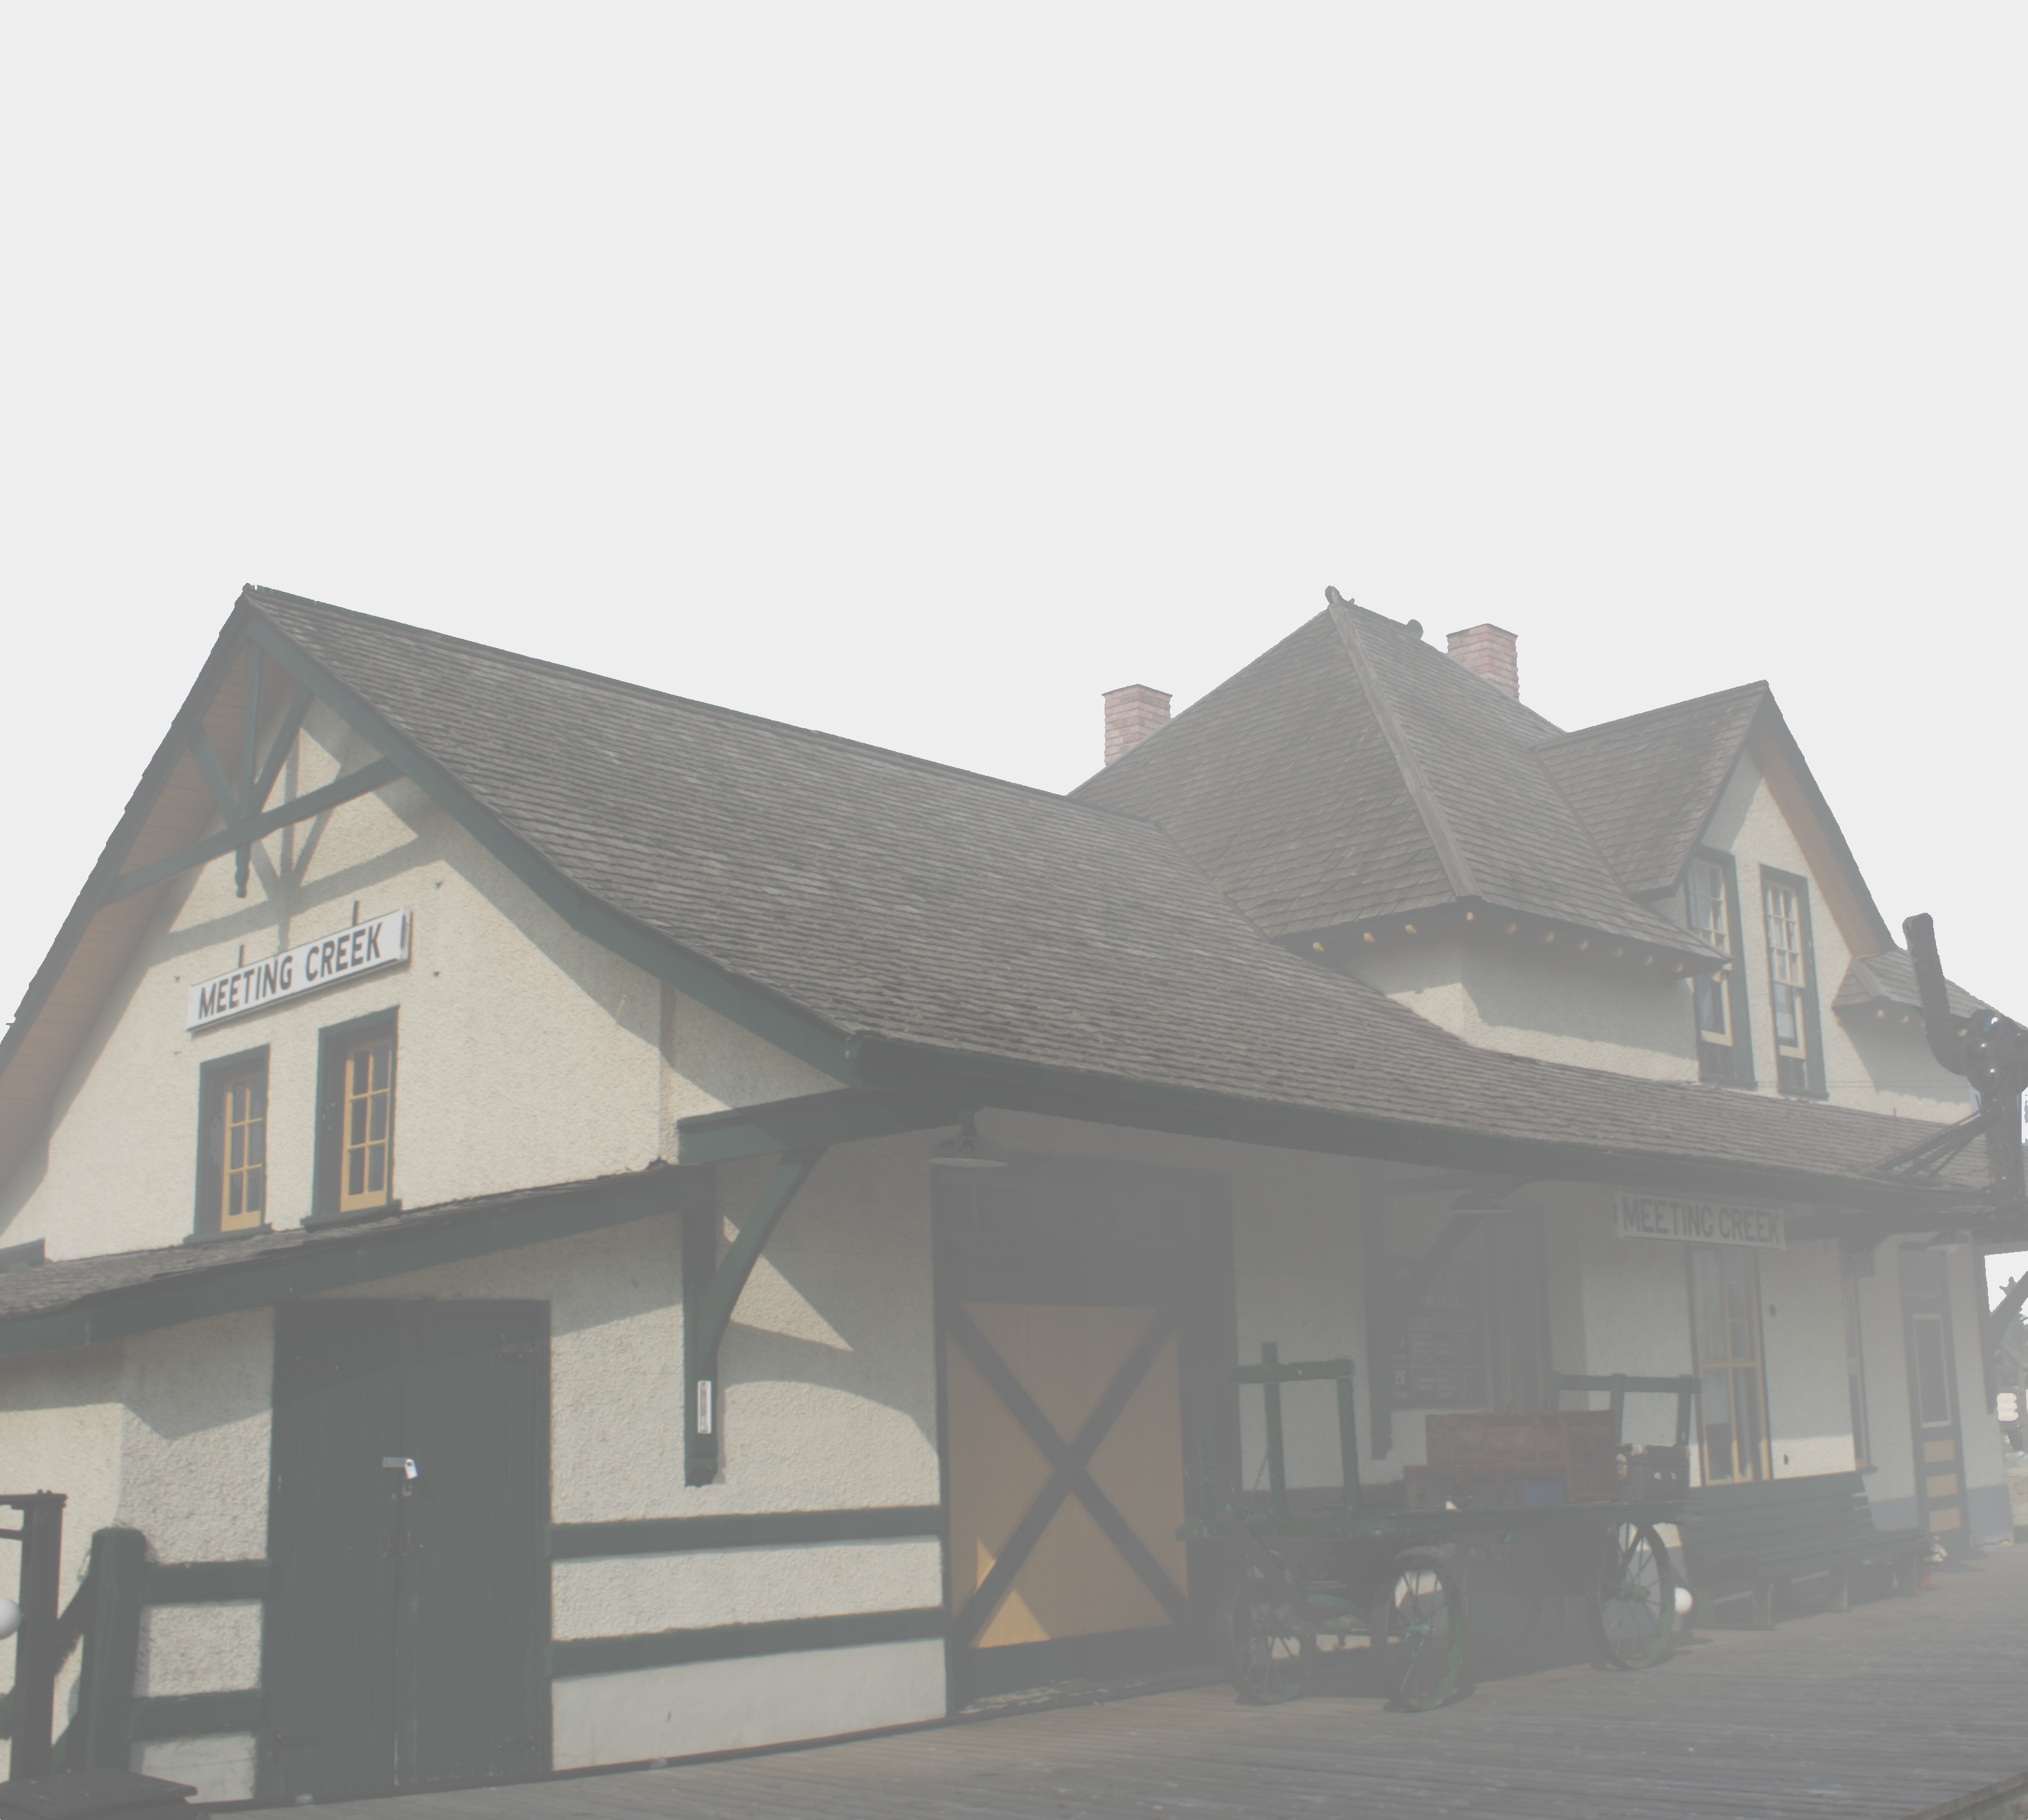
\includegraphics[width=3.2cm]{hazerd/dataset/IMG_8612_200}}
%  \vspace{1.5cm}
%   \centerline{(c)}\medskip
\end{minipage}
\begin{minipage}[b]{0.24\linewidth}
  \centering
  \centerline{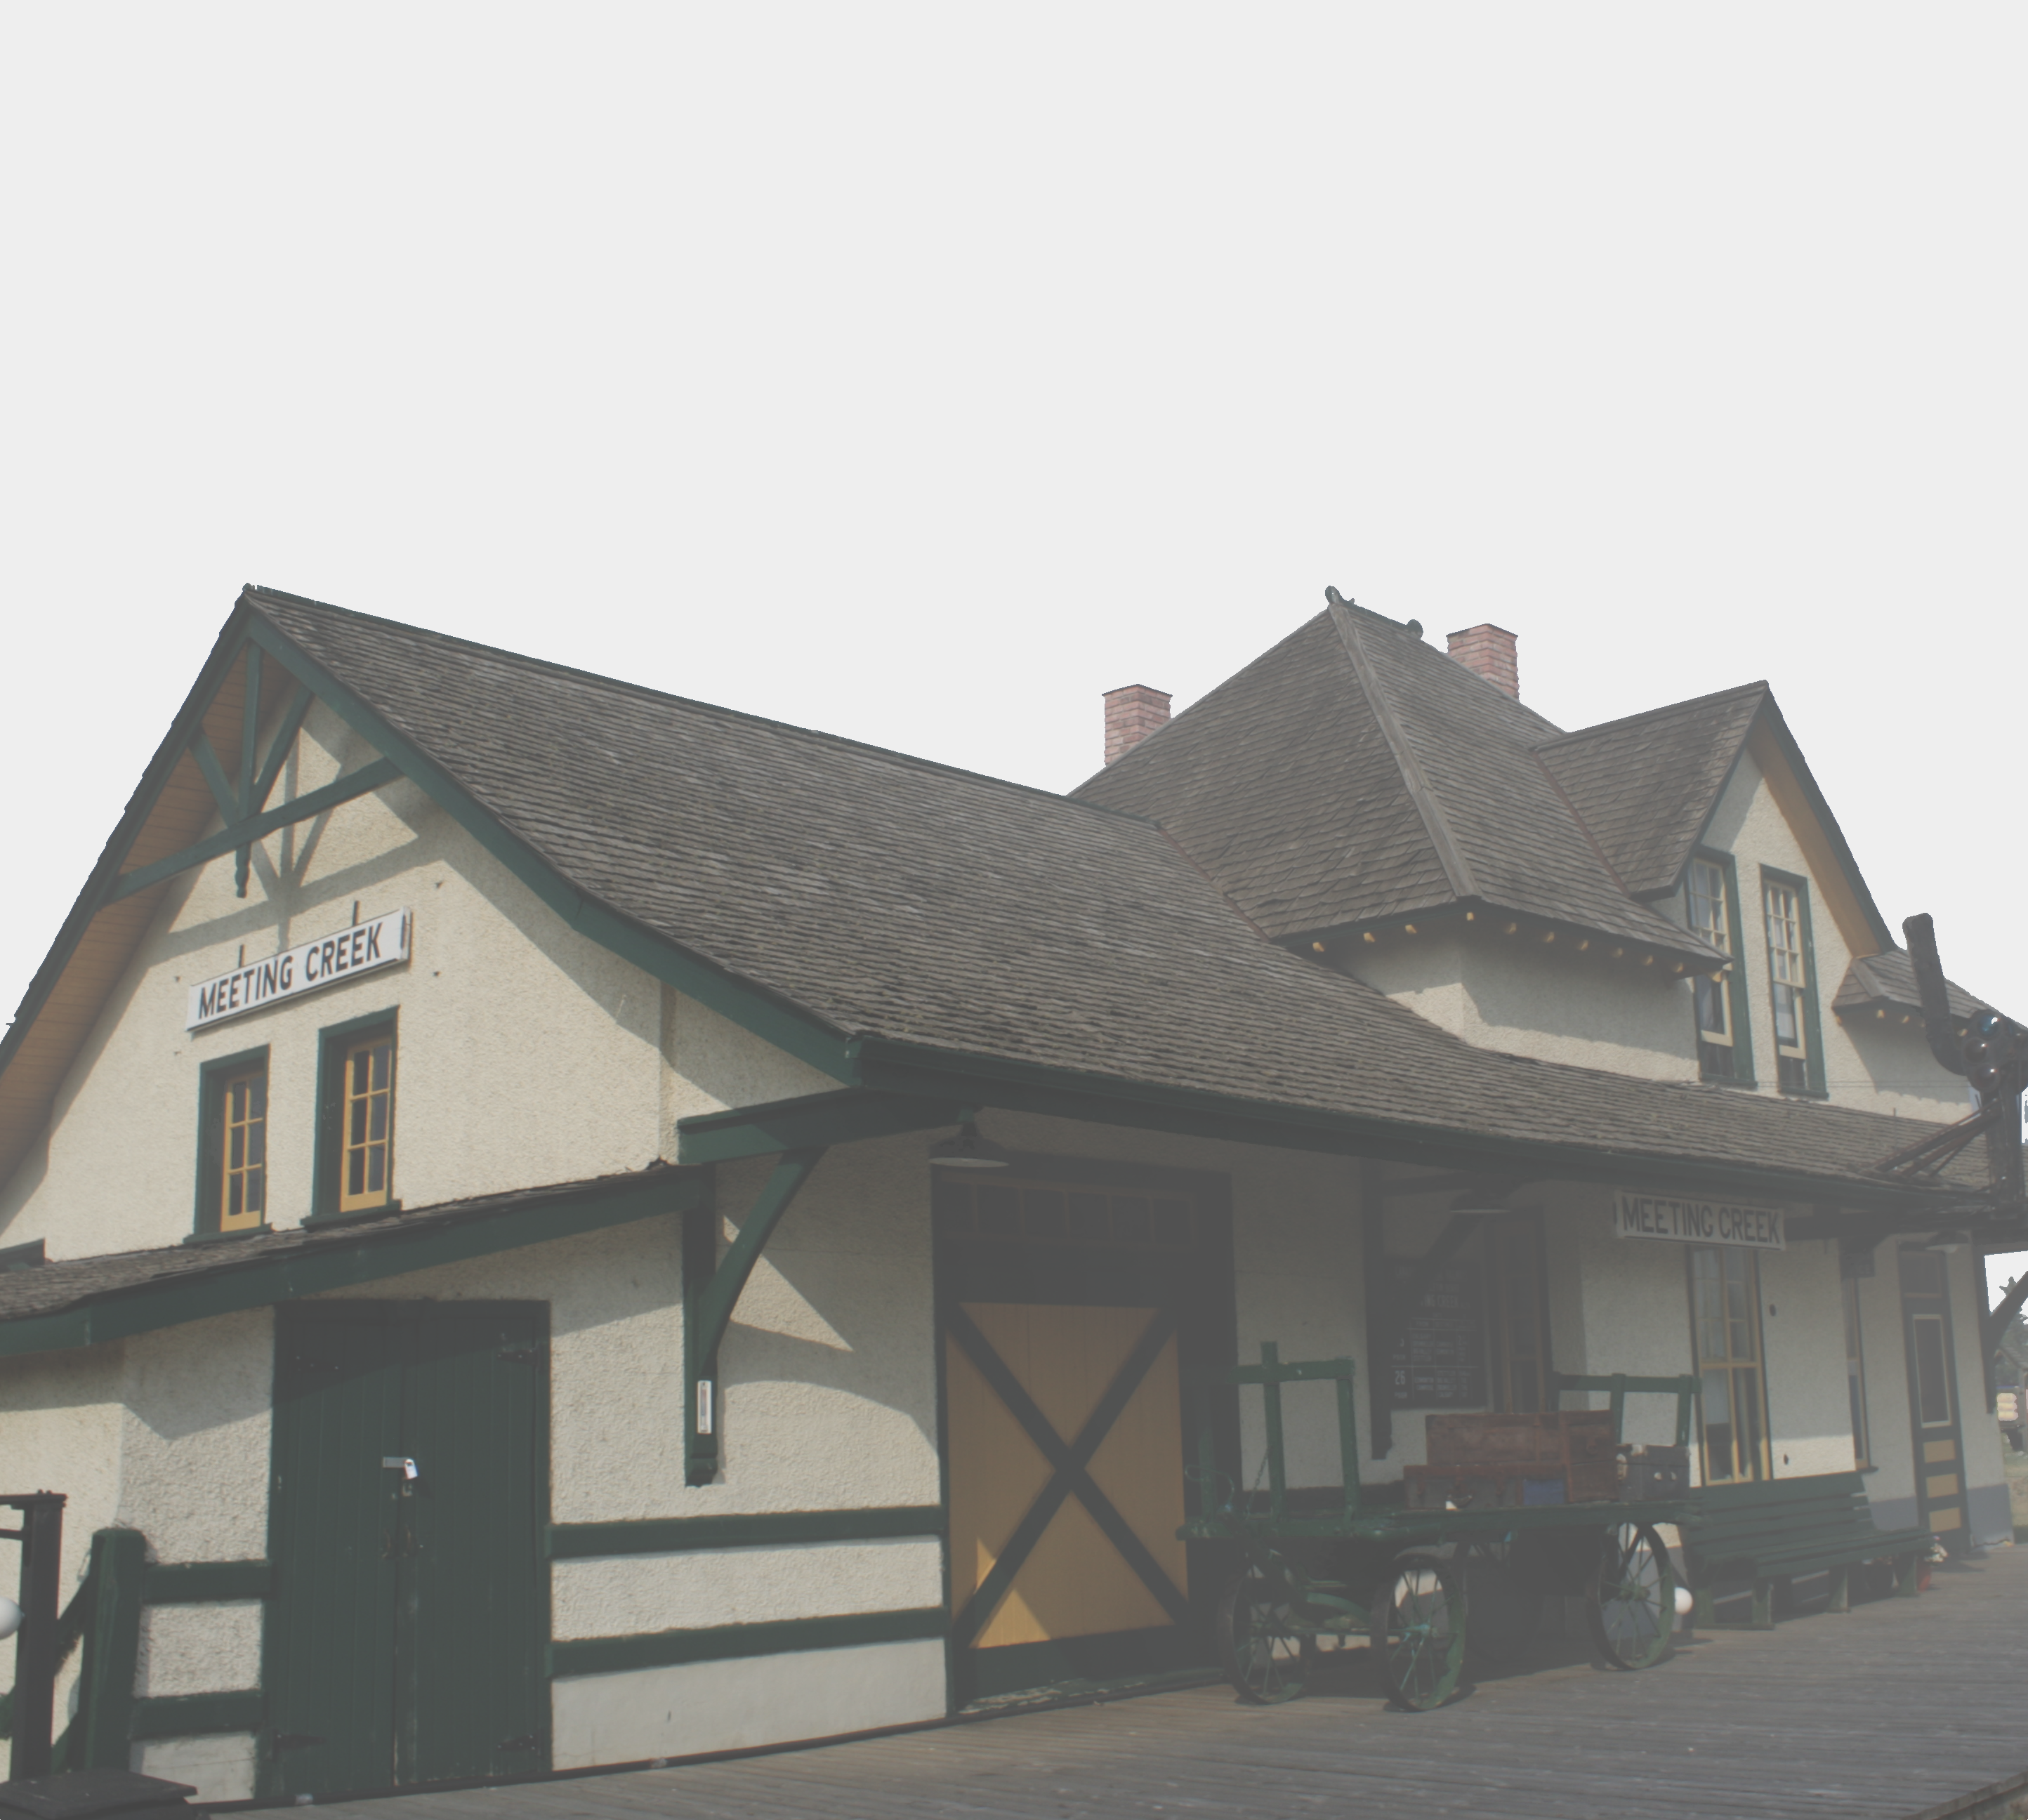
\includegraphics[width=3.2cm]{hazerd/dataset/IMG_8612_500}}
%  \vspace{1.5cm}
%   \centerline{(d)}\medskip
\end{minipage}
\caption{HazeRD Samples. From left to right: a hazy image, with the visual range of 50m, 100m, 200m, and 500m respectively.}
\label{fig:3.example_dataset}
\end{figure}
\begin{figure}[htb]
\centering
\resizebox{0.95\textwidth}{!}{
\begin{minipage}[b]{0.54\linewidth}
  \centering \centerline{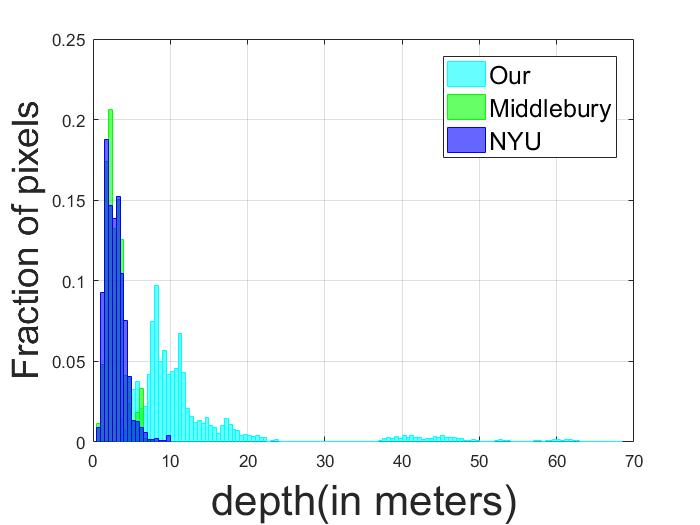
\includegraphics[width=9cm]{hazerd/hist/hist_all}}
%   \centerline{(a)}\medskip
 \end{minipage}
\begin{minipage}[b]{0.44\linewidth}
  \centering \centerline{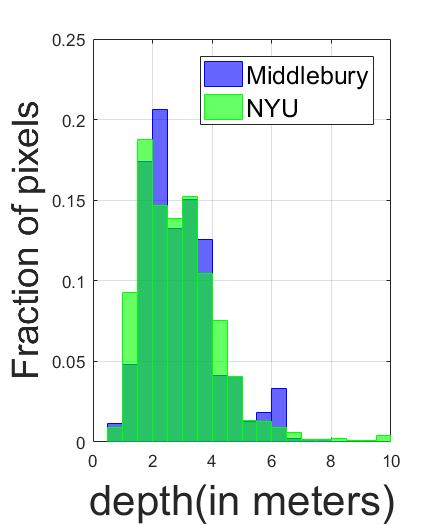
\includegraphics[width=5.5cm]{hazerd/hist/hist_mn}}
%   \centerline{(b)}\medskip
 \end{minipage}}
\caption{Histograms of 3 dataset. Left: HazeRD, Middlebury, and NYU, right: the Middlebury dataset and NYU.}
\label{fig:3.hist_compare}
\end{figure}

\section{benchmark: algorithms and datasets}
\label{sec:3.5.benchmark}
As mentioned above, a typical dehazing algorithm usually has two stages: first, some priors or constraints are formulated to regularize the underconstrained problem, then a loss function is minimized to determine a solution; which is then refined using the hazy images, mainly to eliminate halos or artificial details. In this section, we benchmark six state of art dehazing algorithms described in the following, which we referred to by the labels corresponding to the first author's last name as: (1) He~\cite{he2011single}, (2) Meng~\cite{meng2013efficient}, (3) Zhu~\cite{zhu2015fast}, (4) Berman~\cite{berman2016non}, (5) Cai~\cite{cai2016dehazenet} and (6) Ren~\cite{Ren-ECCV-2016}.
% \begin{itemize}
%     \item He~\cite{he2011single}
%     \item Meng~\cite{meng2013efficient}
%     \item Zhu~\cite{zhu2015fast}
%     \item Berman~\cite{berman2016non}
%     \item Cai~\cite{cai2016dehazenet}
% \end{itemize}
% We briefly summarize the algorithms in order to subsequently understand their success and failure. Some examples of these techniques on HazeRD and synthesized NYU and Middlebury dataset are showed in Fig.~\ref{fig:exmaple_3dpc} and Fig.~\ref{fig:exmaple_nyu_middlebury}.
We briefly summarize the algorithms in order to subsequently understand their success and failure. Some examples of these techniques on HazeRD and synthesized NYU and Middlebury dataset are showed in Fig.~\ref{fig:3.exmaple.hazerd}, Fig.~\ref{fig:3.exmaple.hazerd.trans}, Fig.~\ref{fig:3.exmaple.nyu}, and Fig.~\ref{fig:3.exmaple.middlebury}.
\begin{figure*}[htb]
\begin{subfigure}[b]{1\linewidth}
  \centering
  \centerline{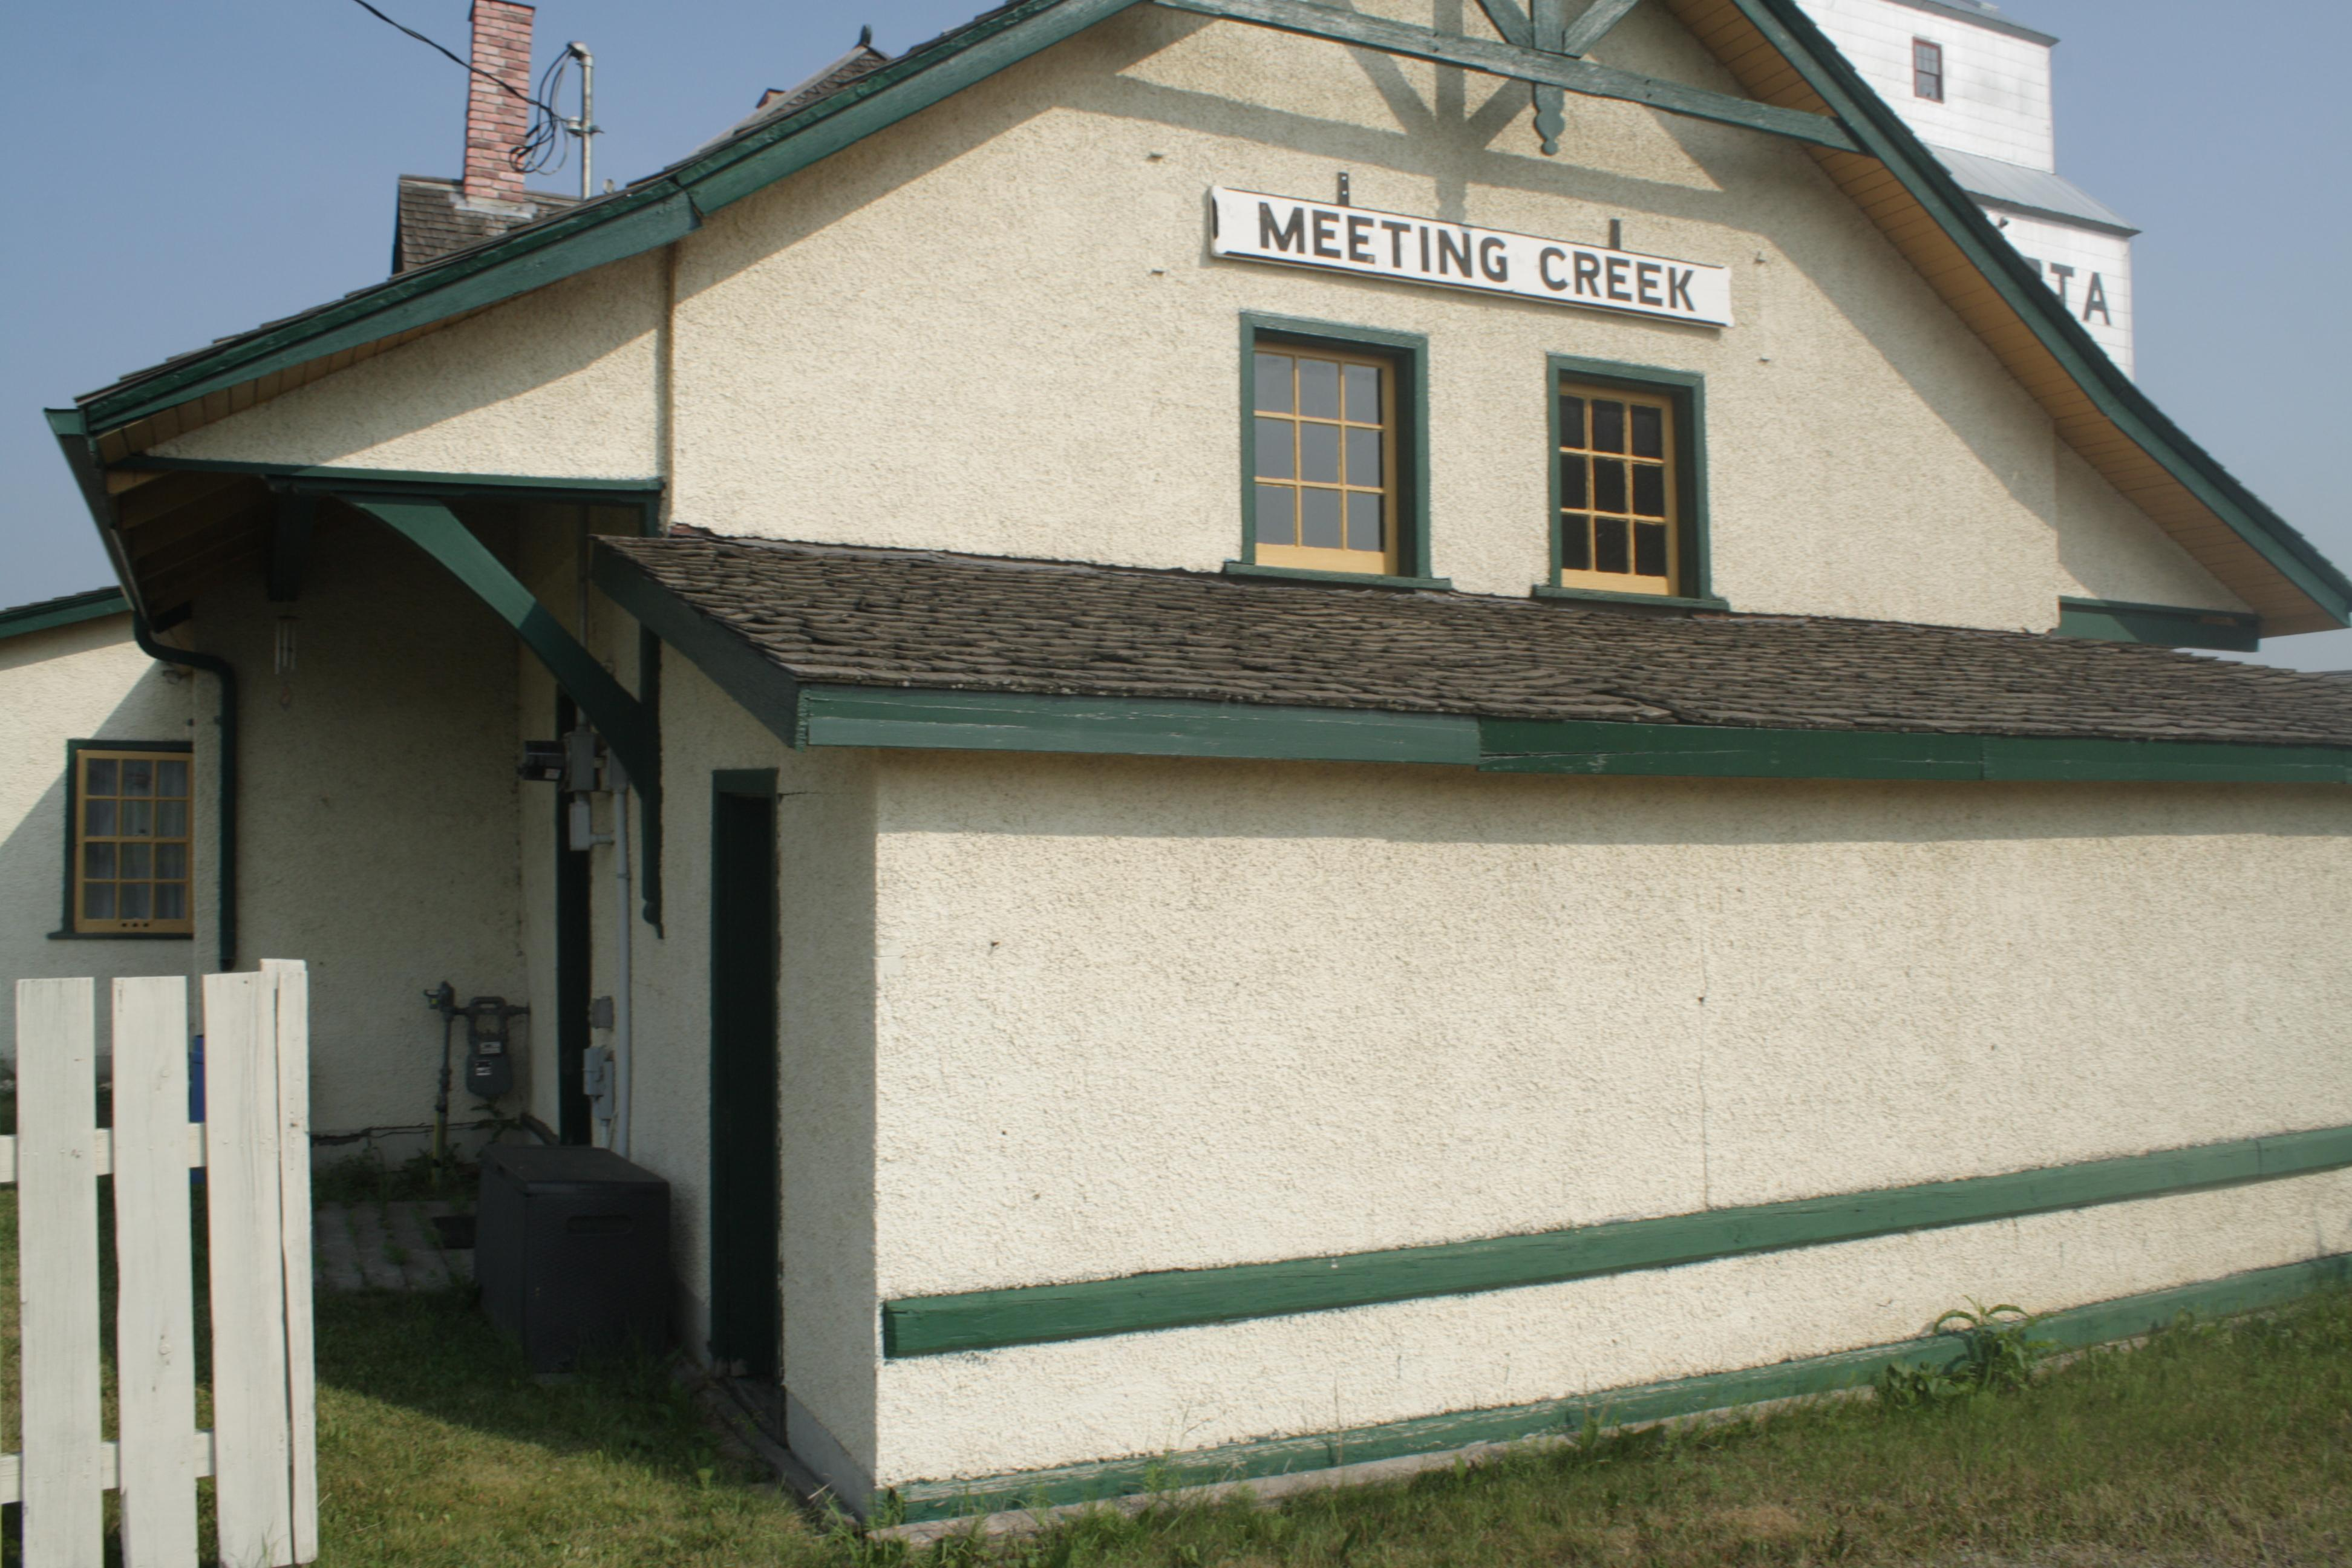
\includegraphics[width=6cm]{hazerd/img/ori_img}}
  \subcaption{}
\end{subfigure}
\vfill
\begin{subfigure}[b]{0.45\linewidth}
  \centering
  \centerline{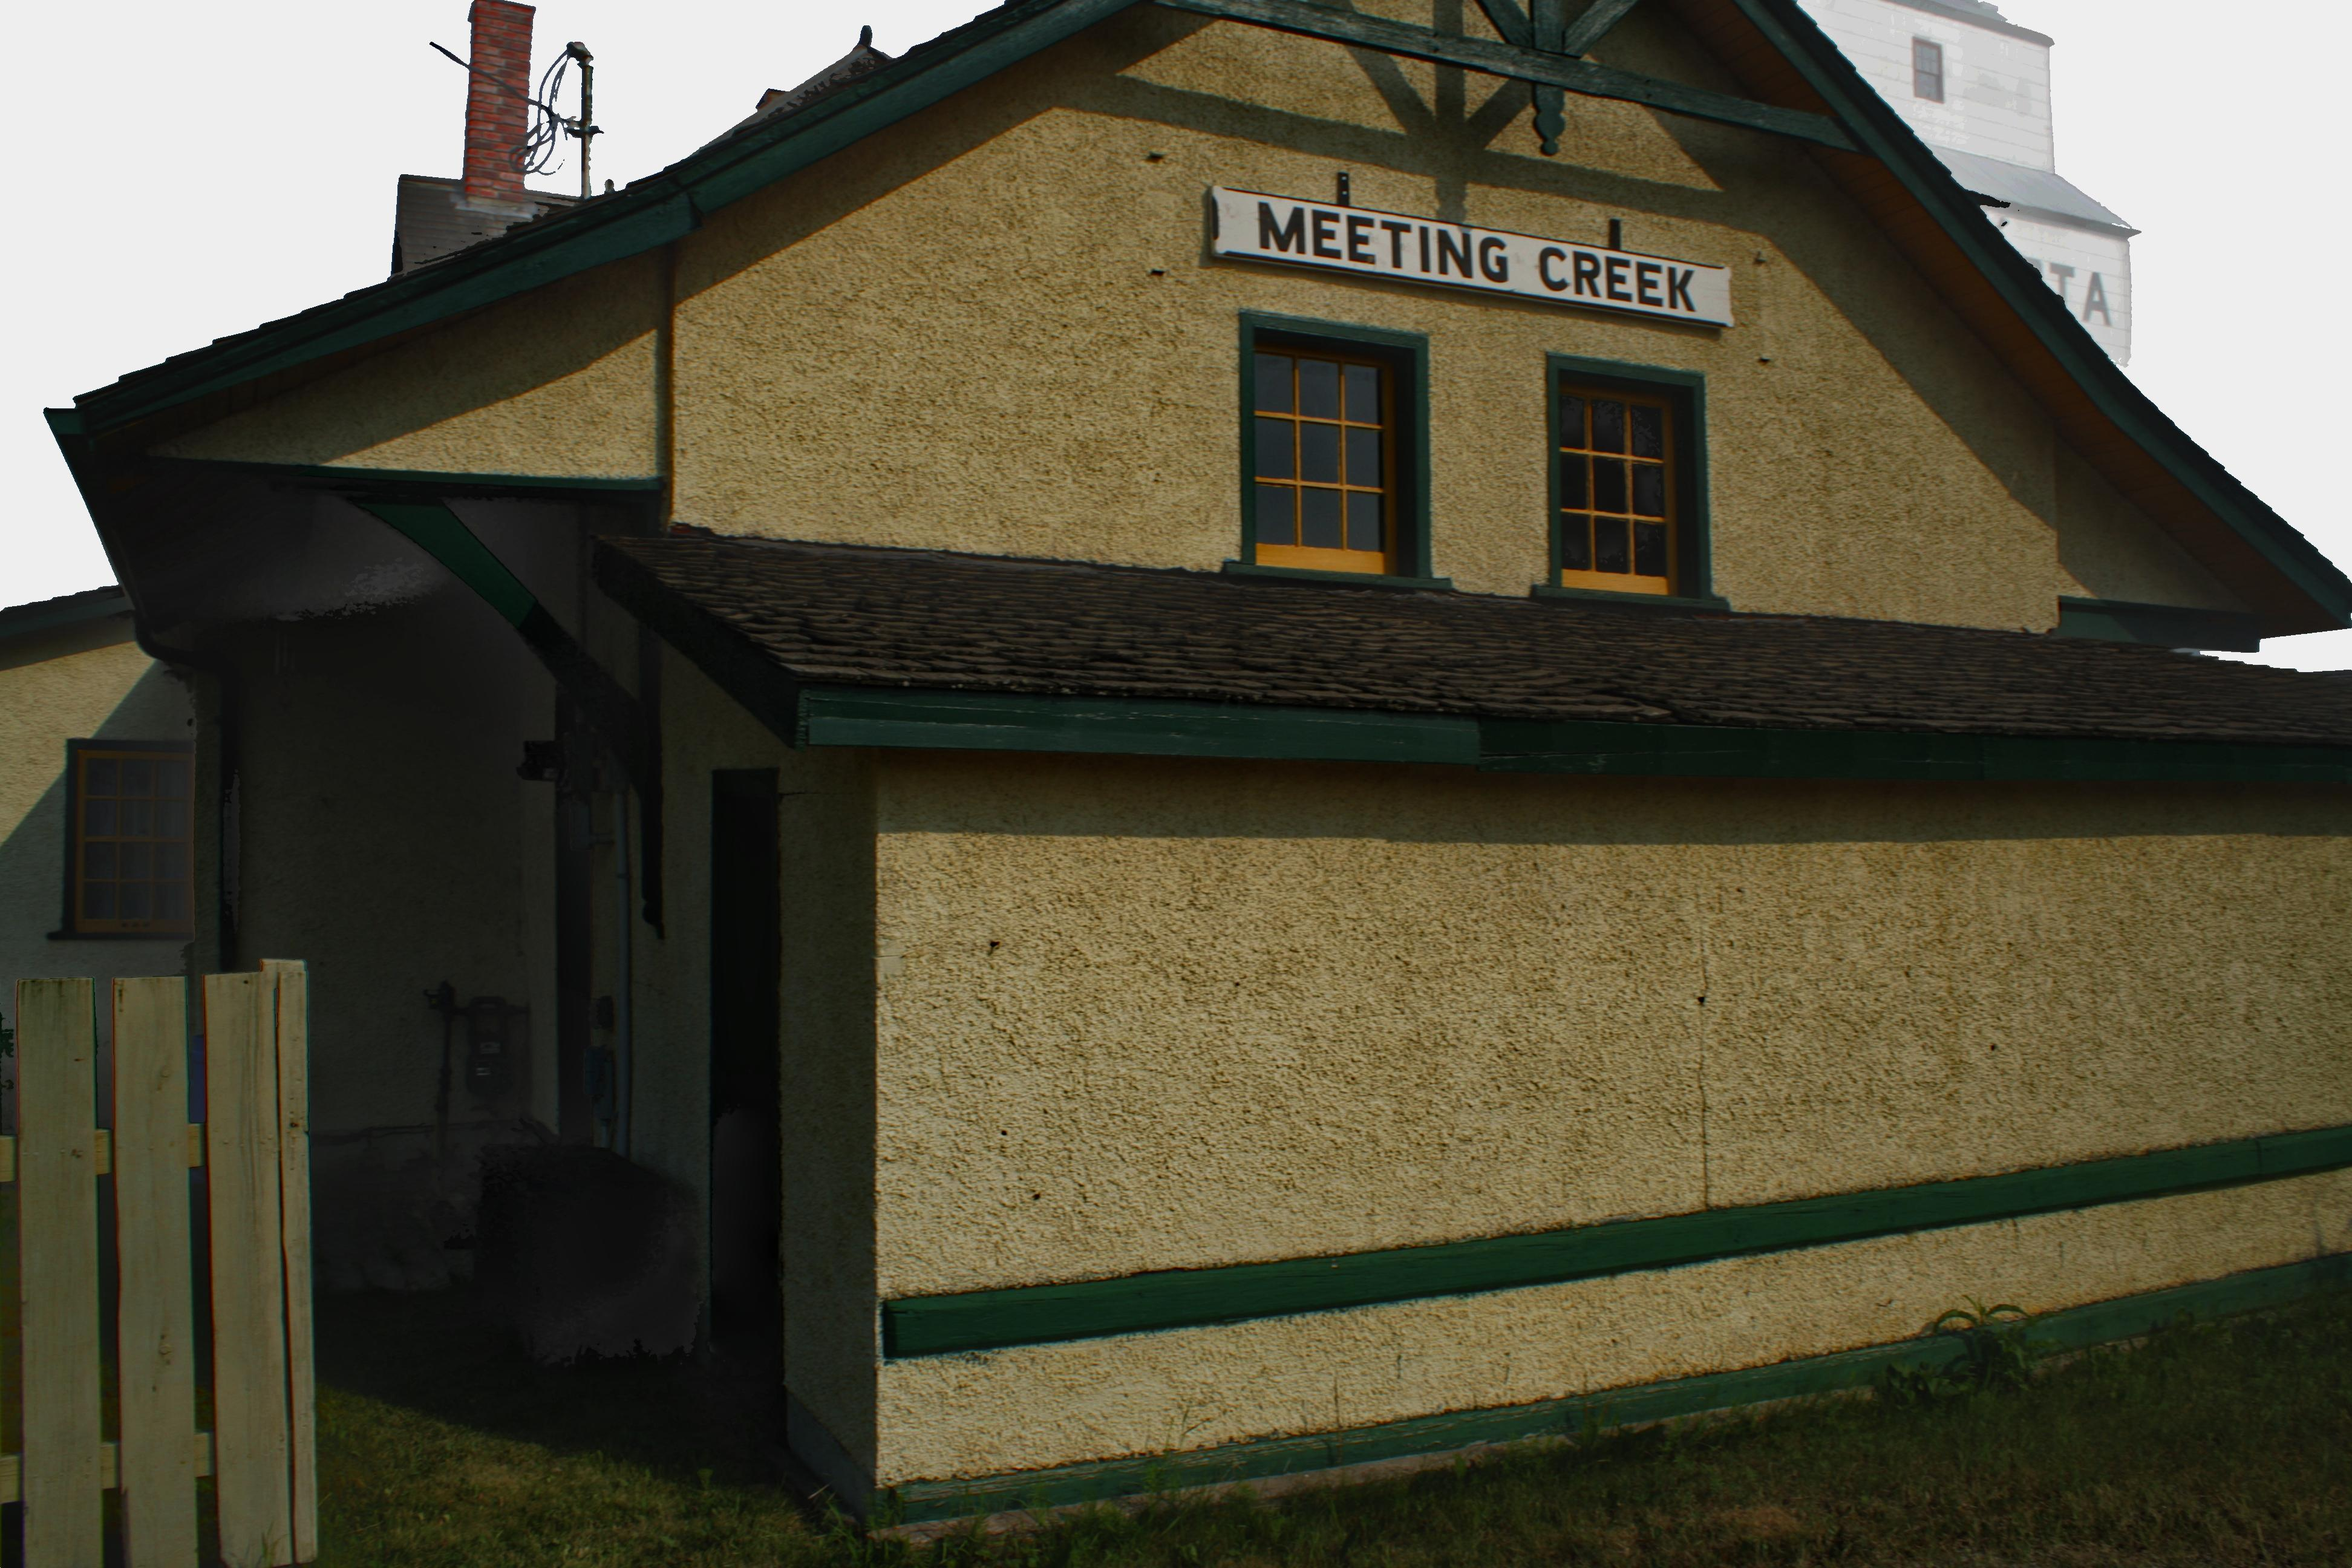
\includegraphics[width=5cm]{hazerd/img/dehaze_he}}
  \subcaption{}
\end{subfigure}
\hfill
\begin{subfigure}[b]{0.45\linewidth}
  \centering
  \centerline{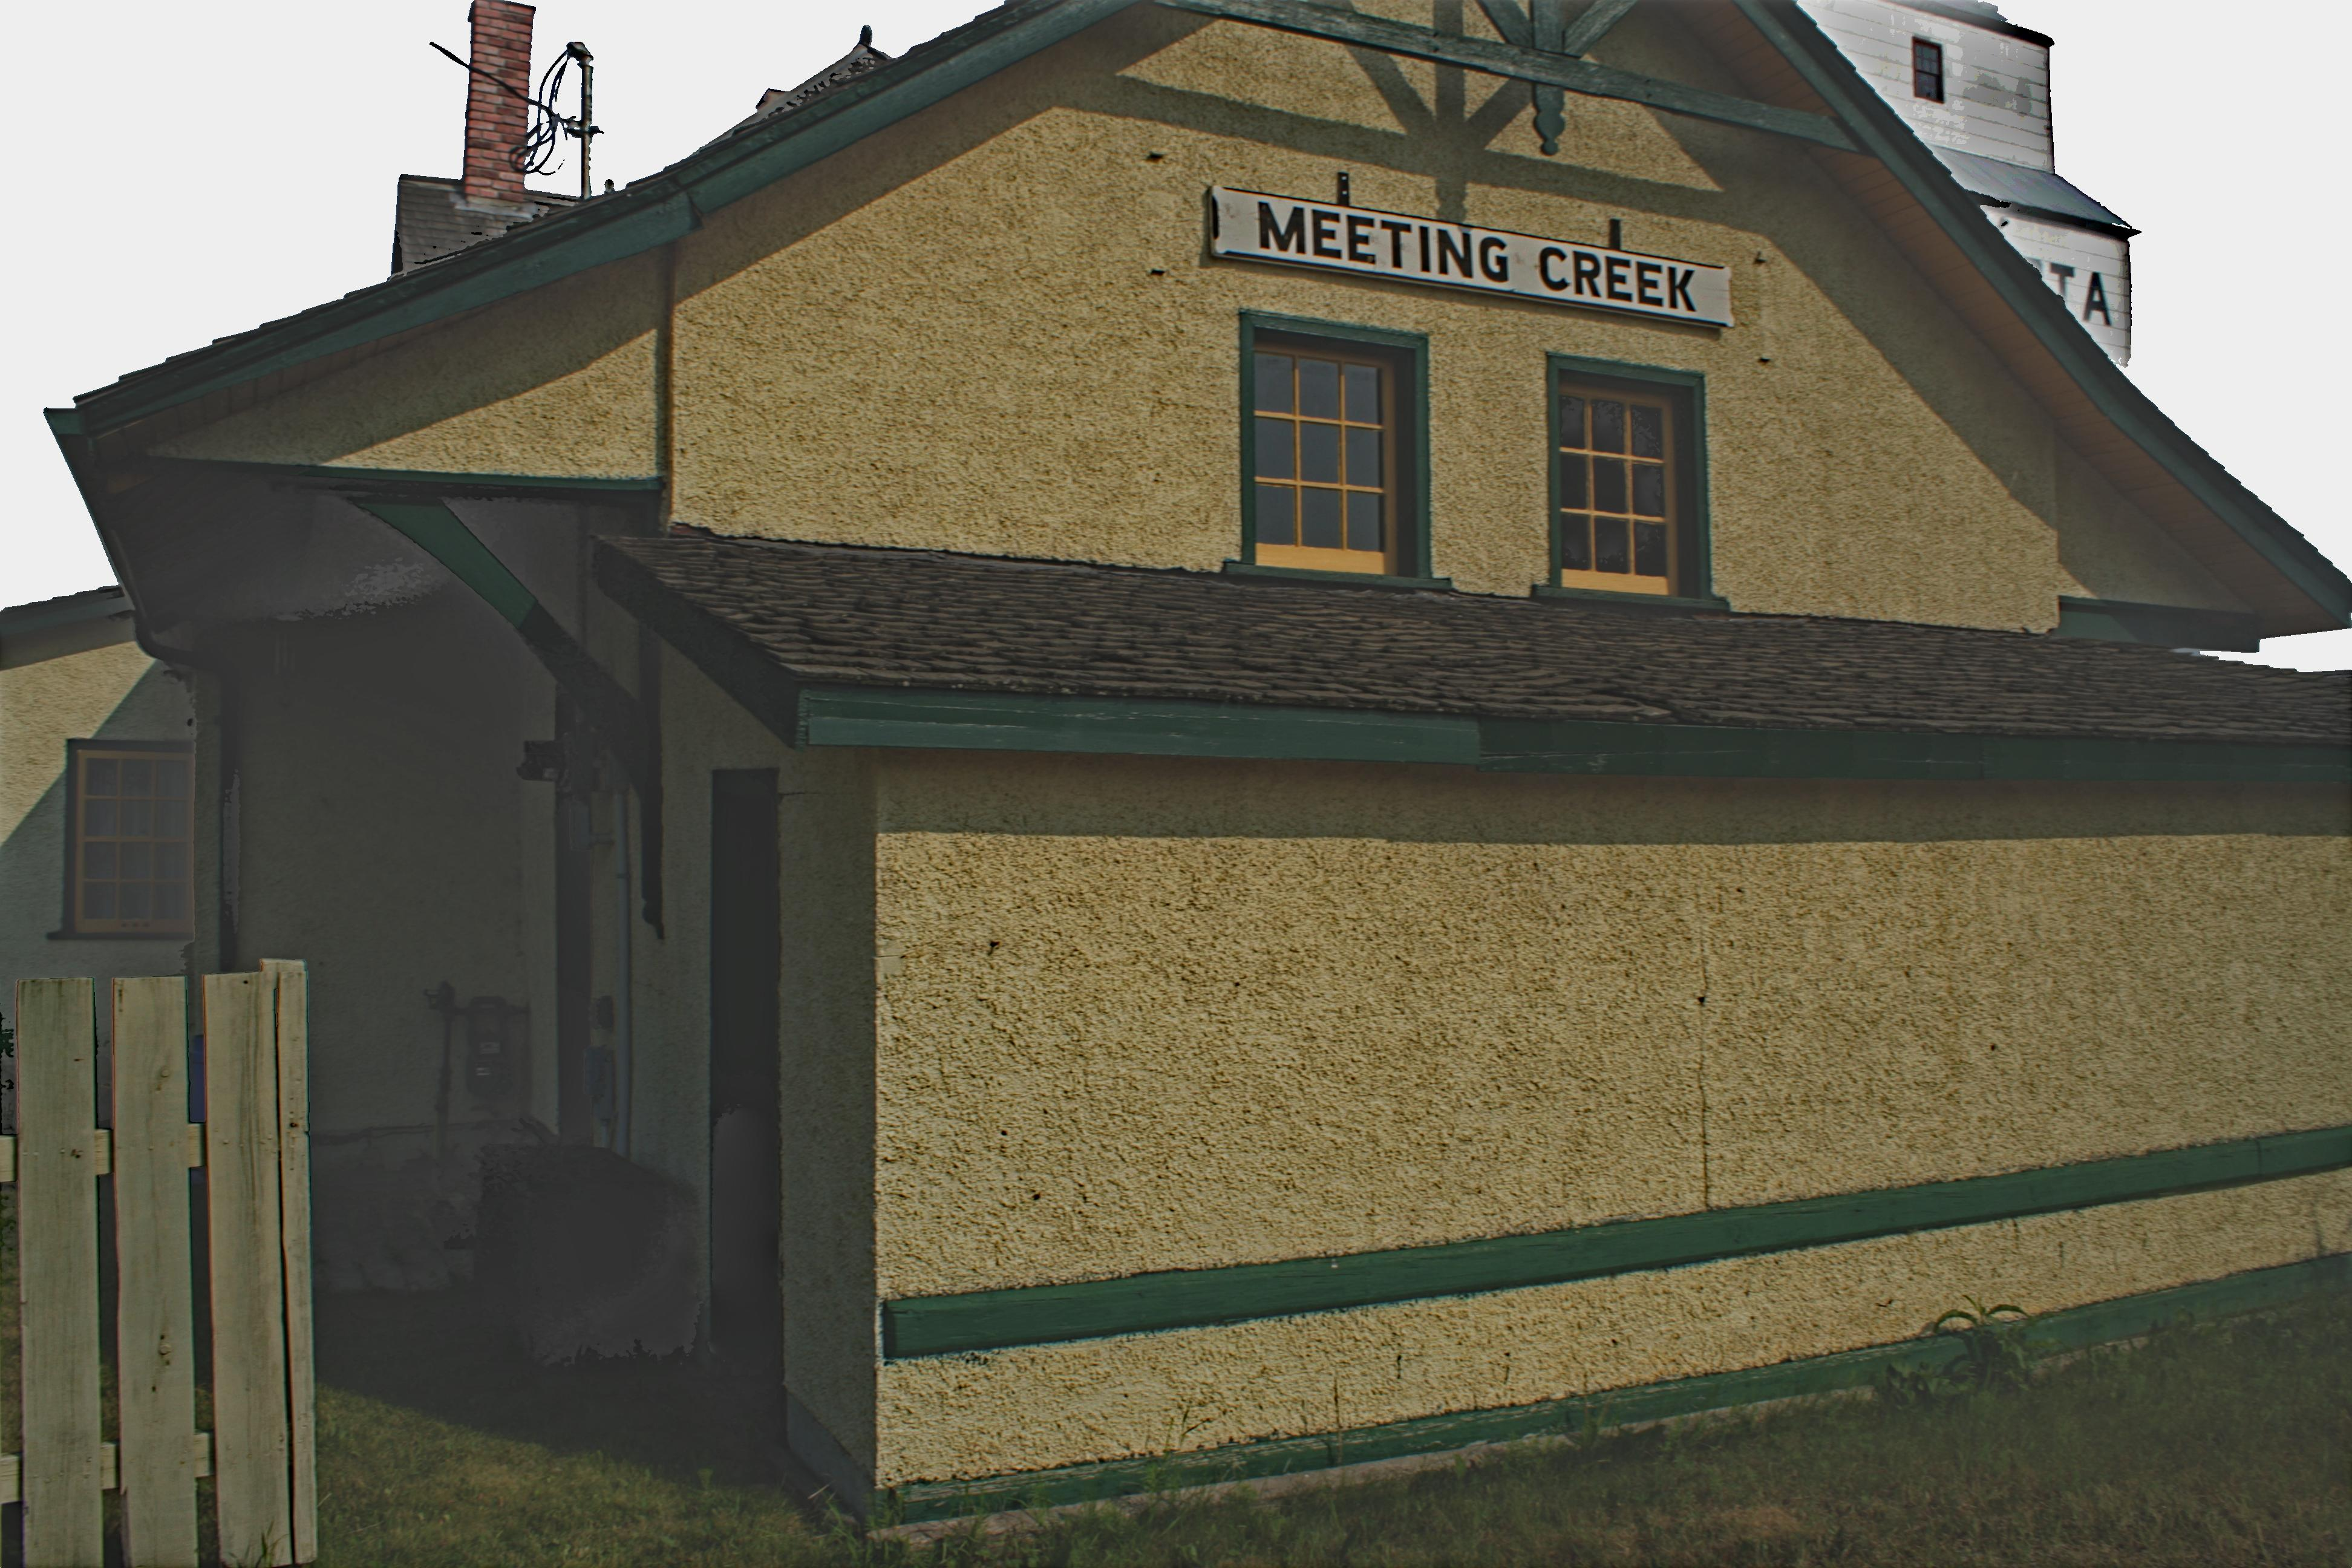
\includegraphics[width=5cm]{hazerd/img/dehaze_meng}}
  \subcaption{}
\end{subfigure}
\vfill
\begin{subfigure}[b]{0.45\linewidth}
  \centering
  \centerline{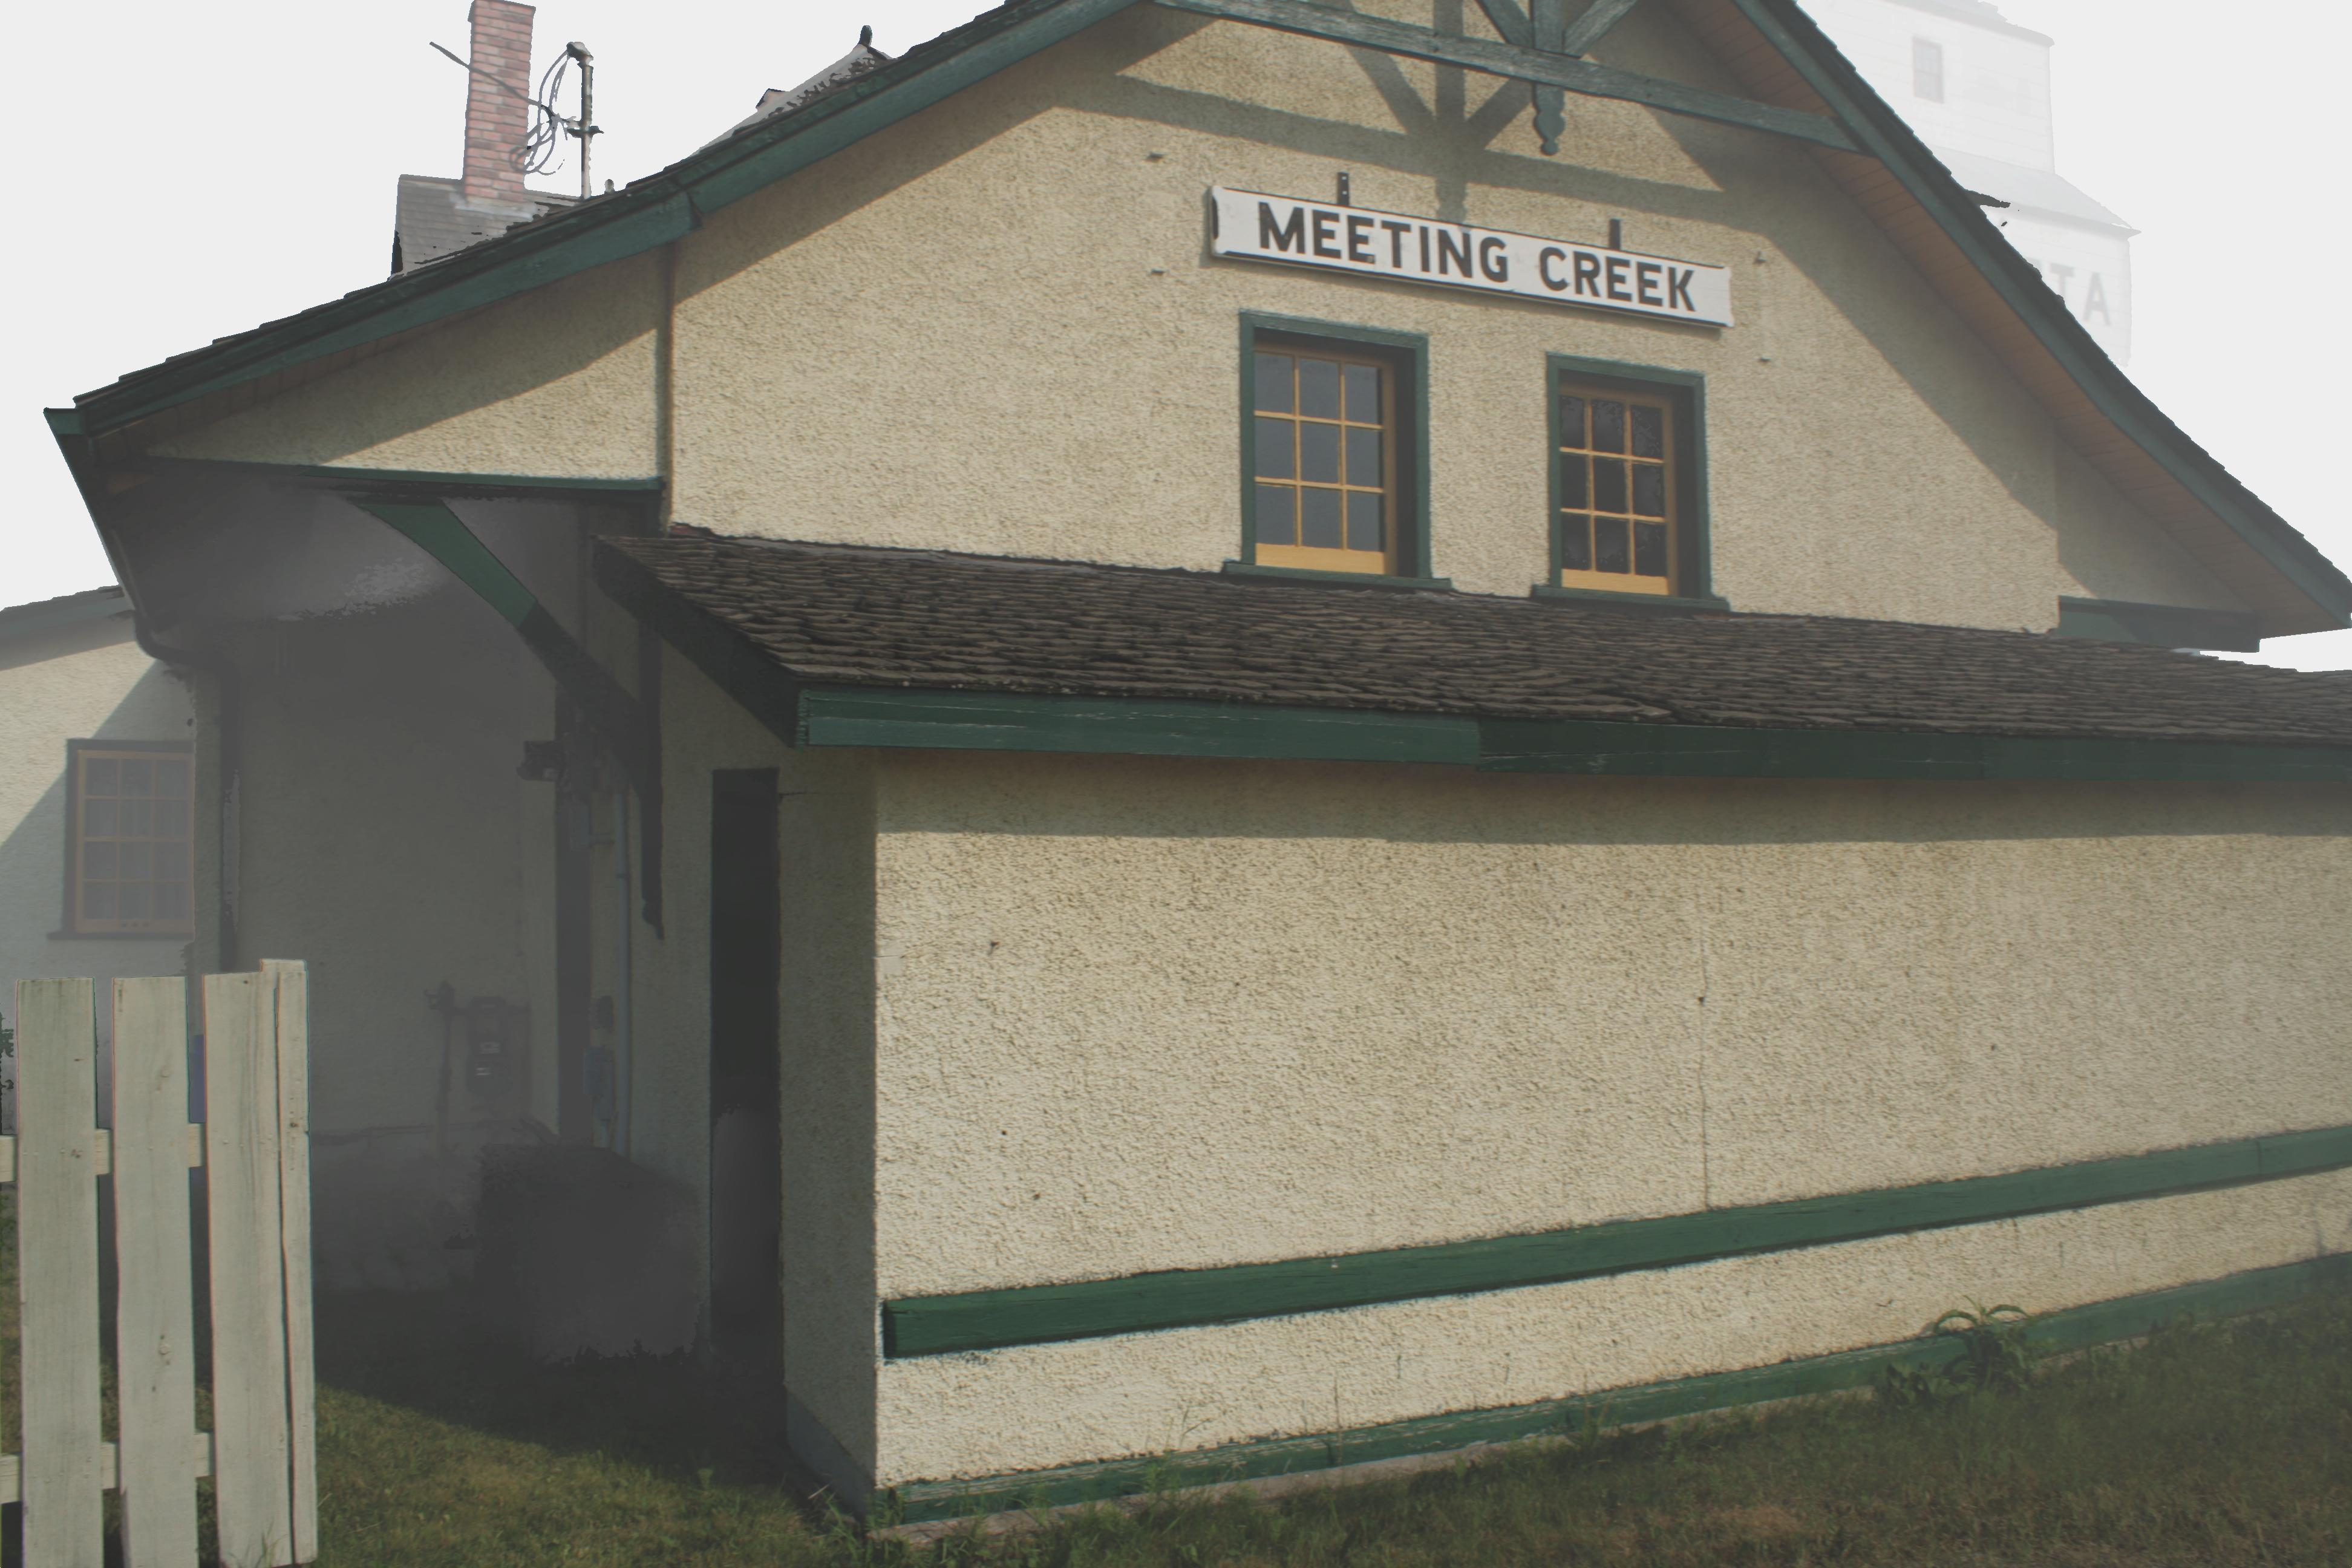
\includegraphics[width=5cm]{hazerd/img/dehaze_zhu}}
  \subcaption{}
\end{subfigure}
\hfill
\begin{subfigure}[b]{0.45\linewidth}
  \centering
  \centerline{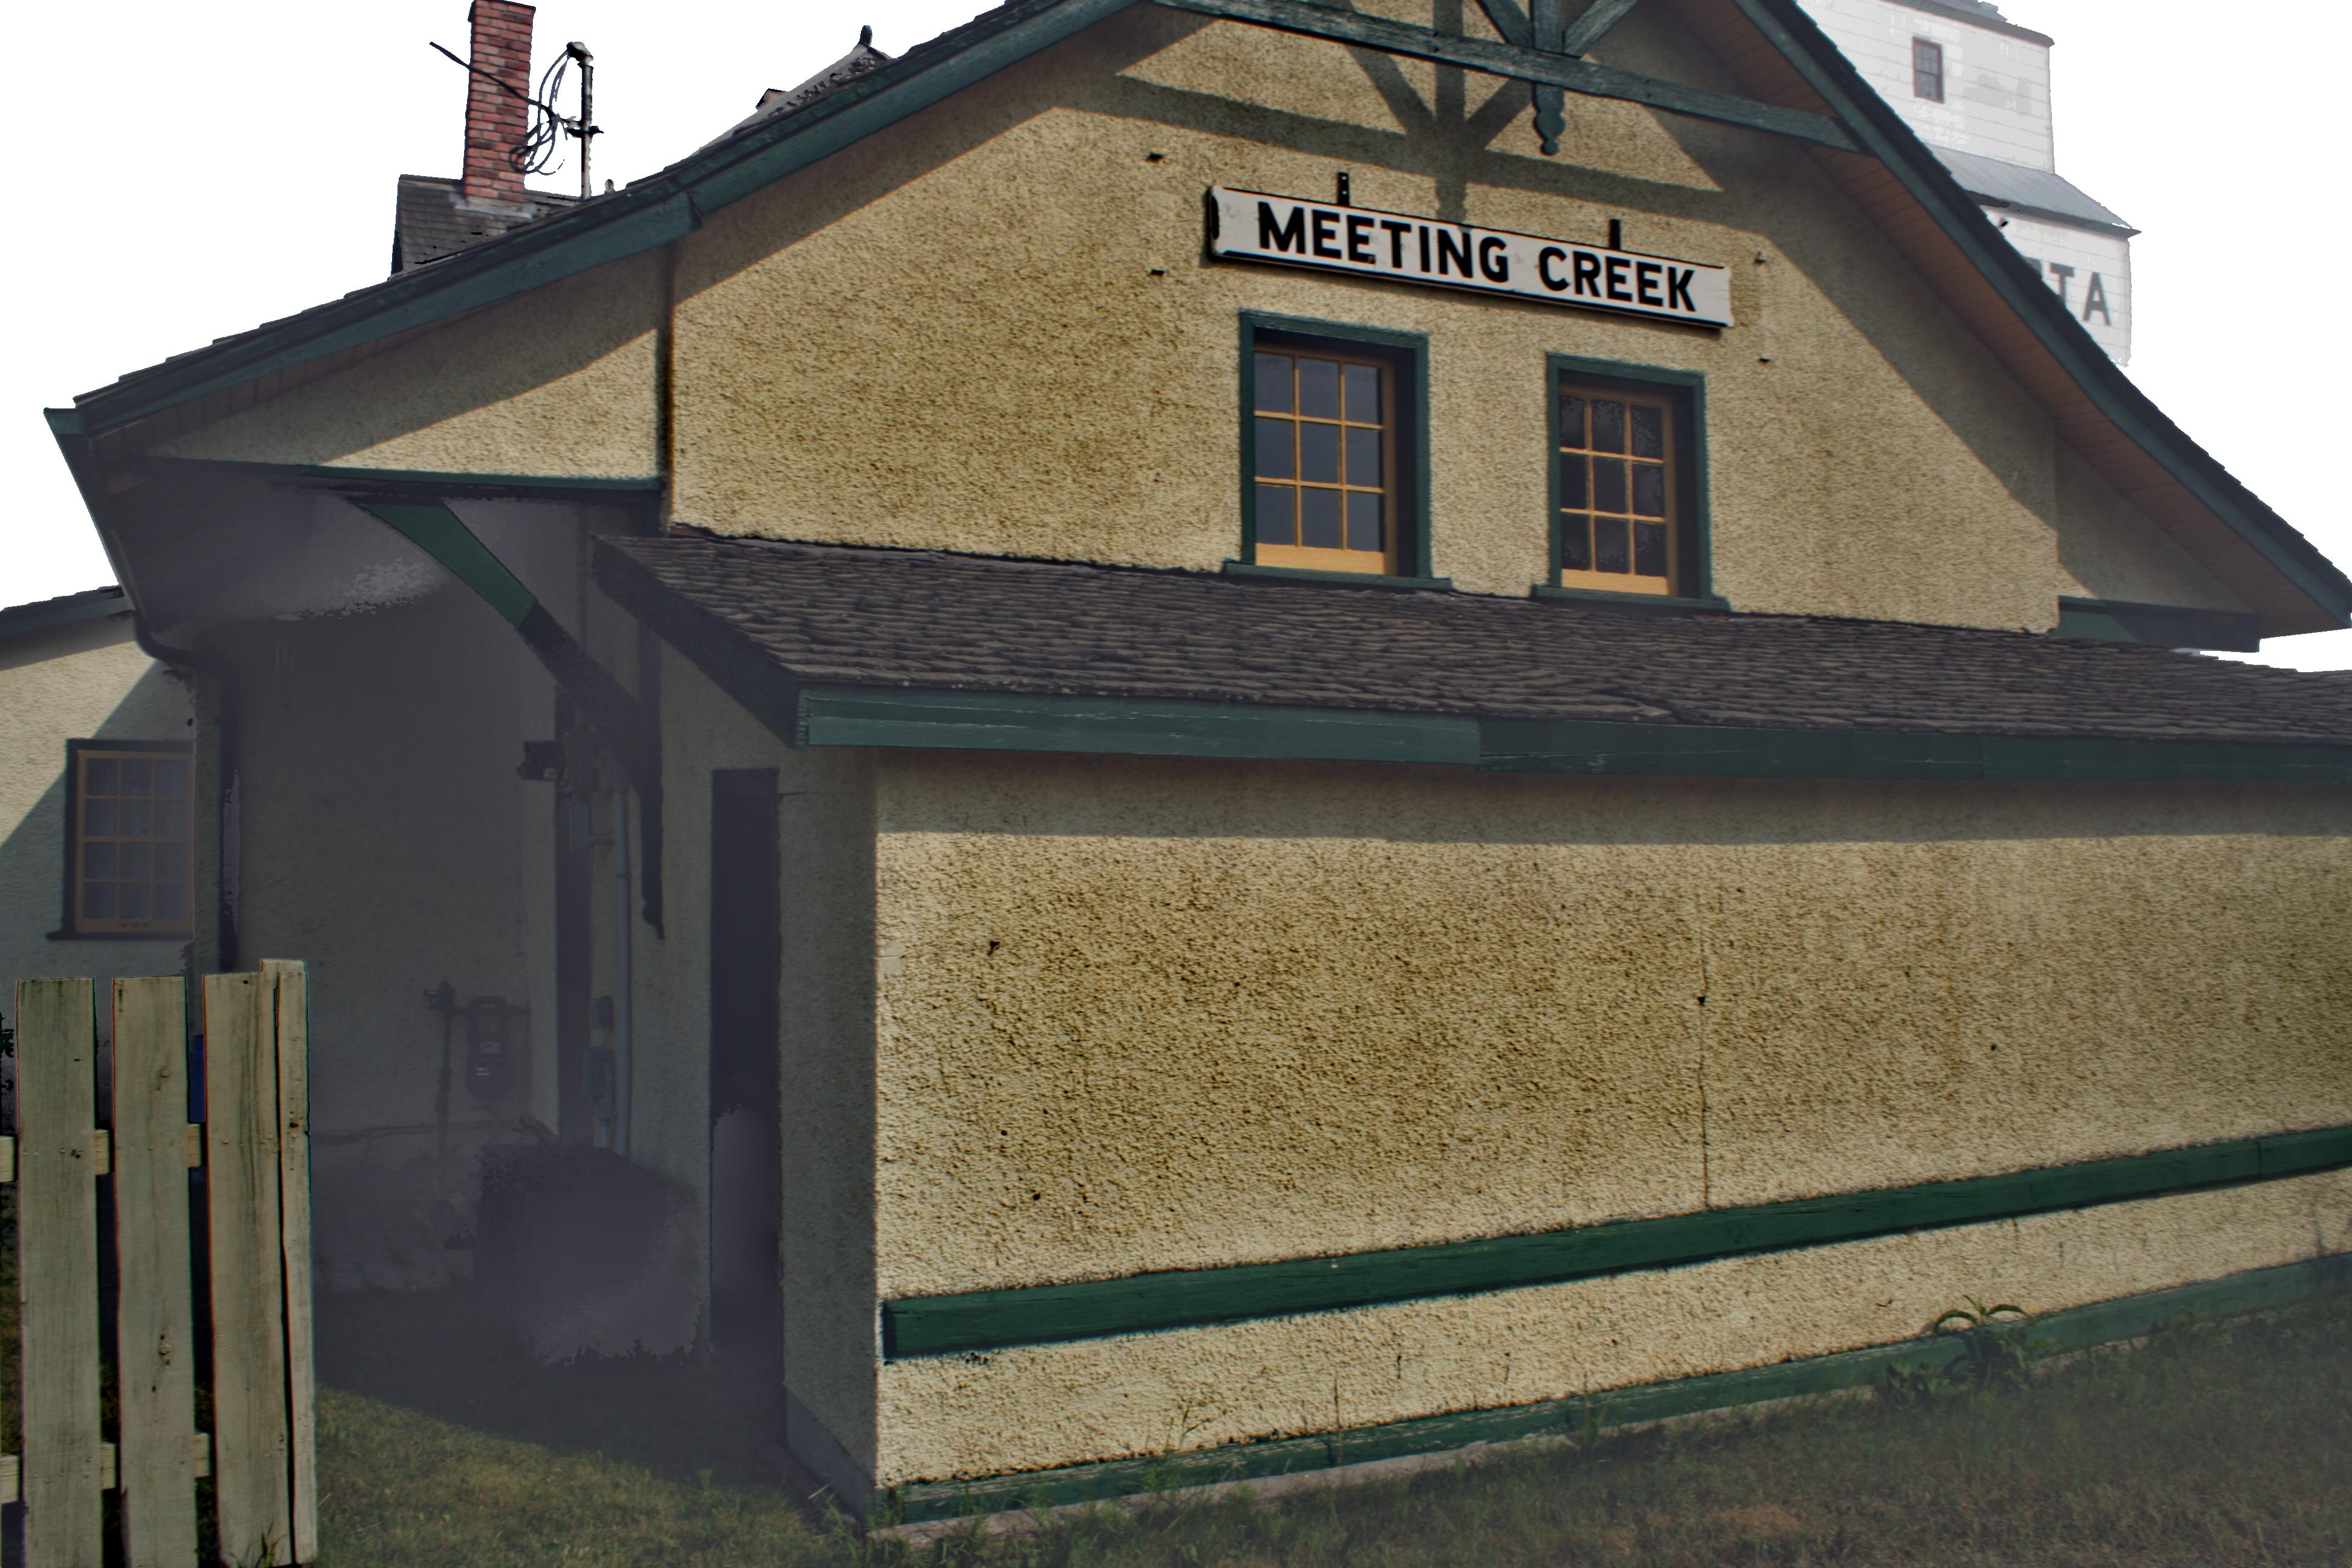
\includegraphics[width=5cm]{hazerd/img/dehaze_berman}}
  \subcaption{}
\end{subfigure}
\vfill
\begin{subfigure}[b]{0.45\linewidth}
  \centering
  \centerline{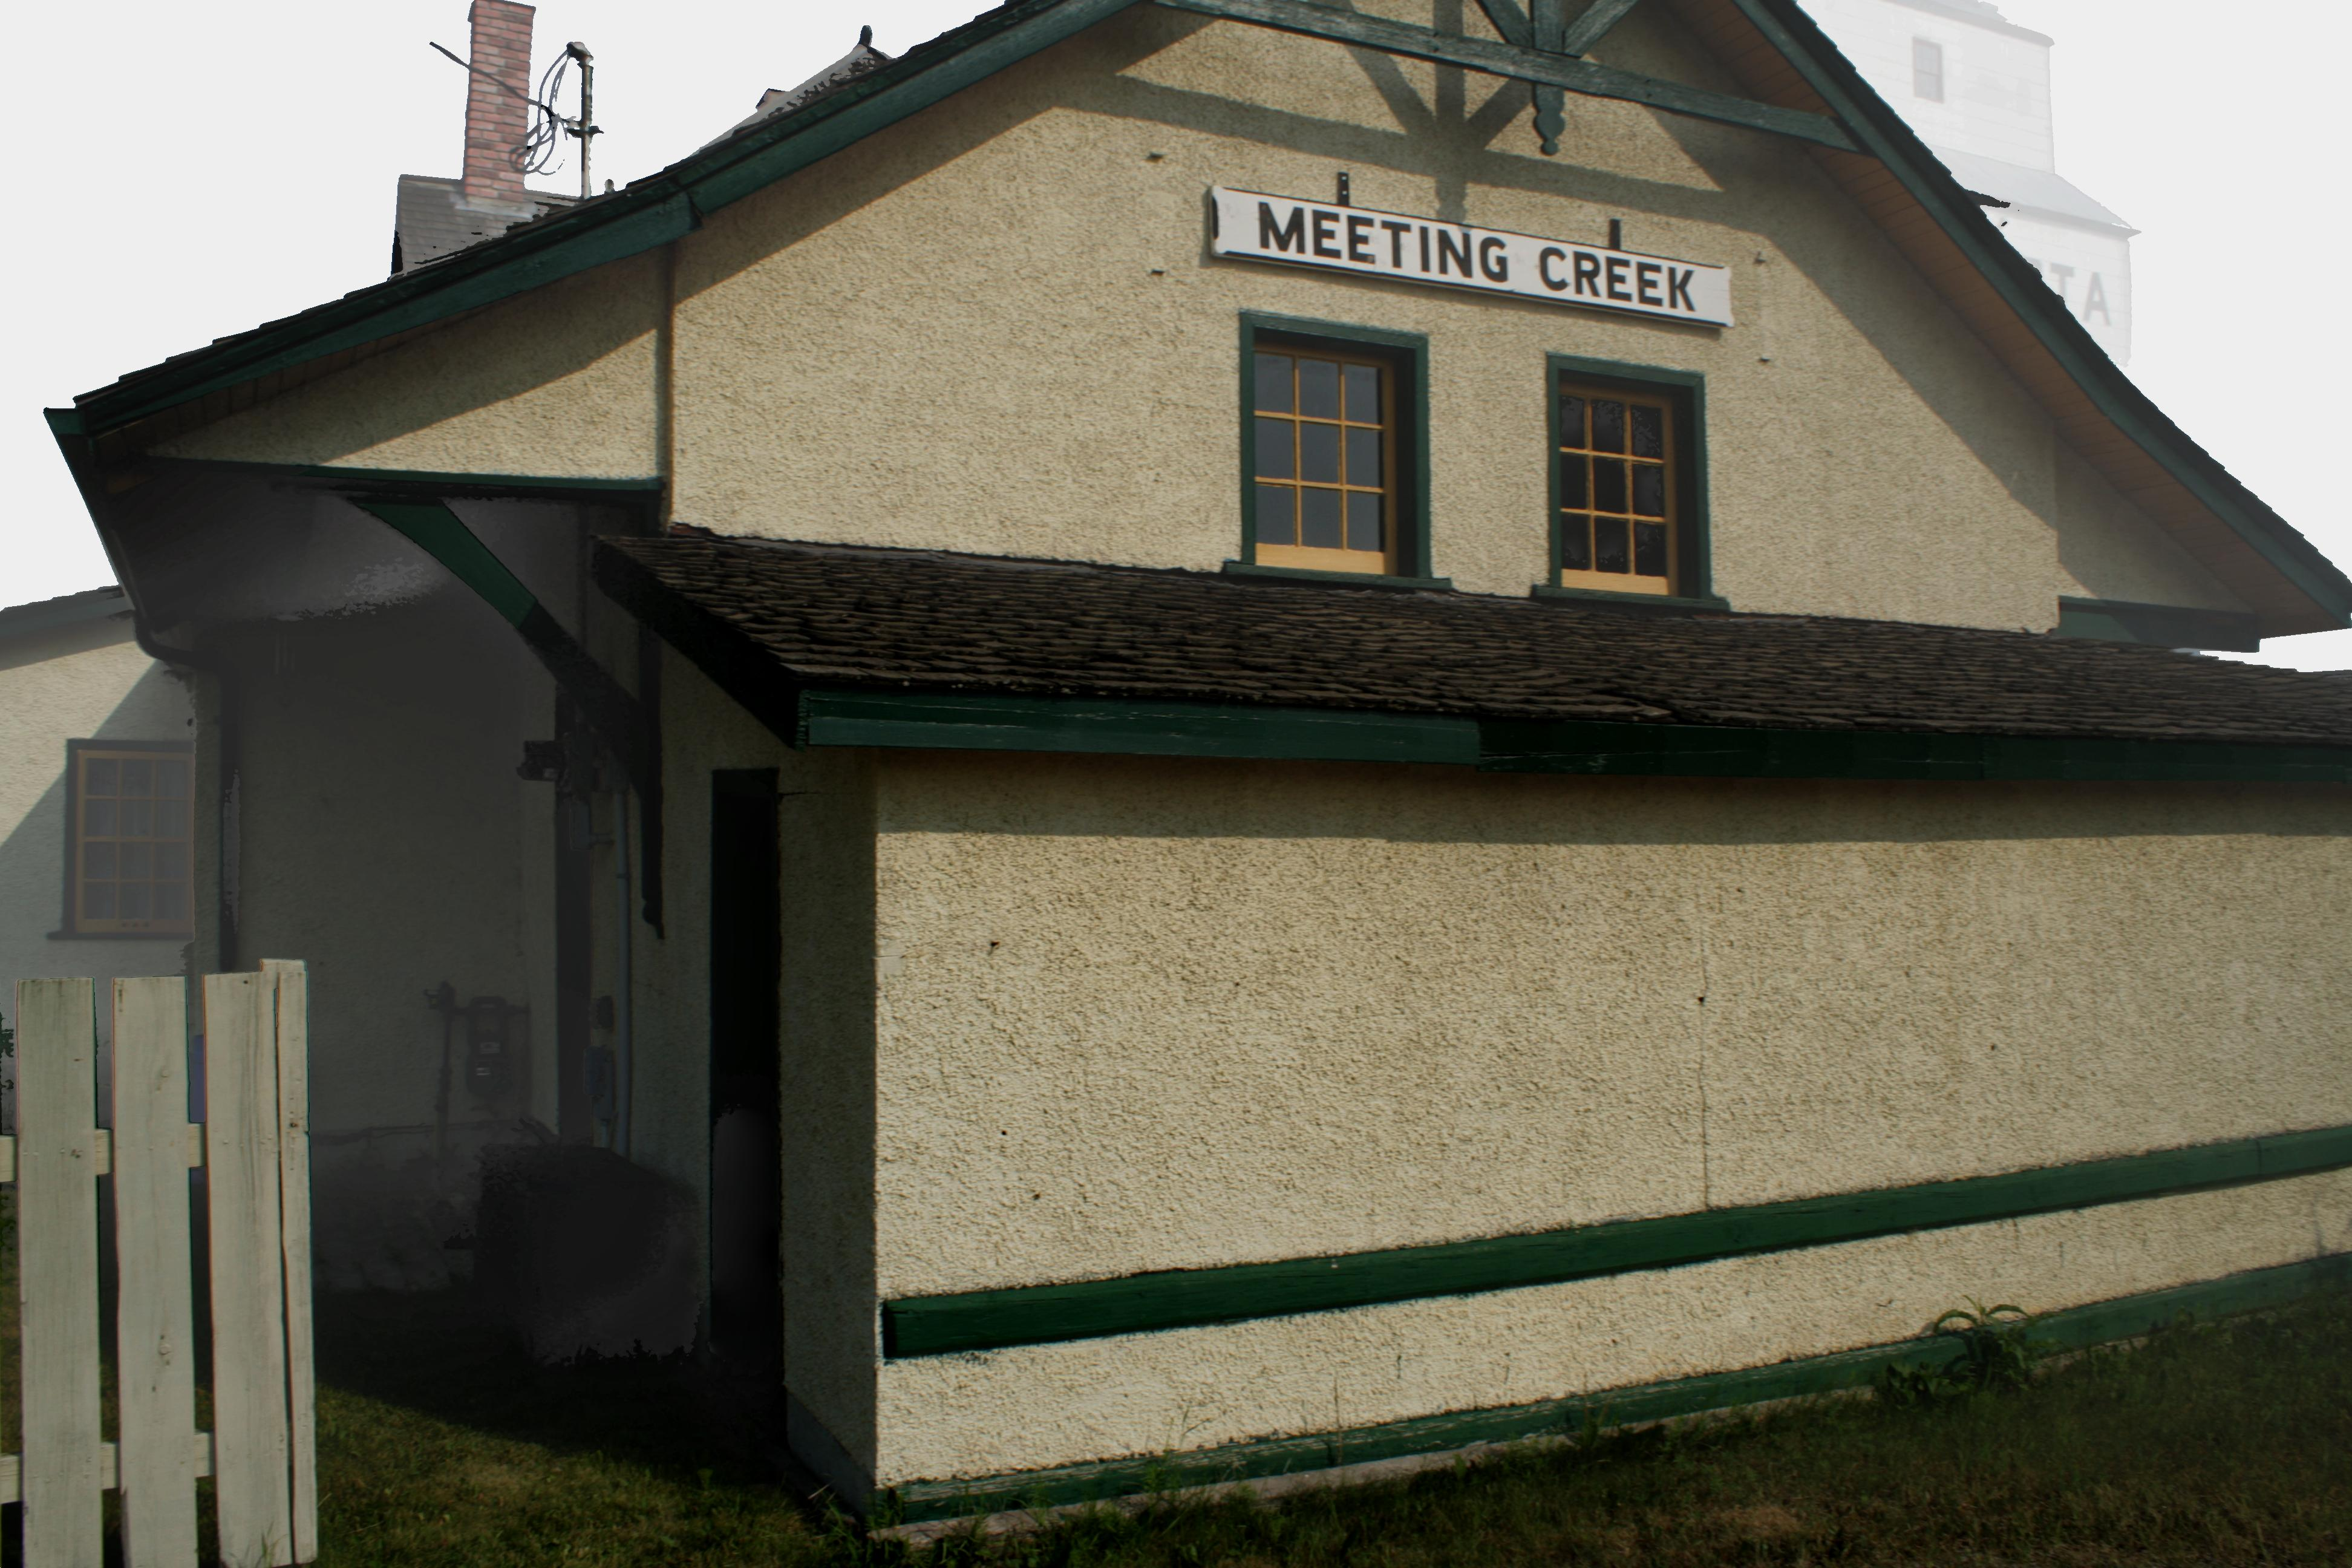
\includegraphics[width=5cm]{hazerd/img/dehaze_cai}}
  \subcaption{}
\end{subfigure}
\hfill
\begin{subfigure}[b]{0.45\linewidth}
  \centering
  \centerline{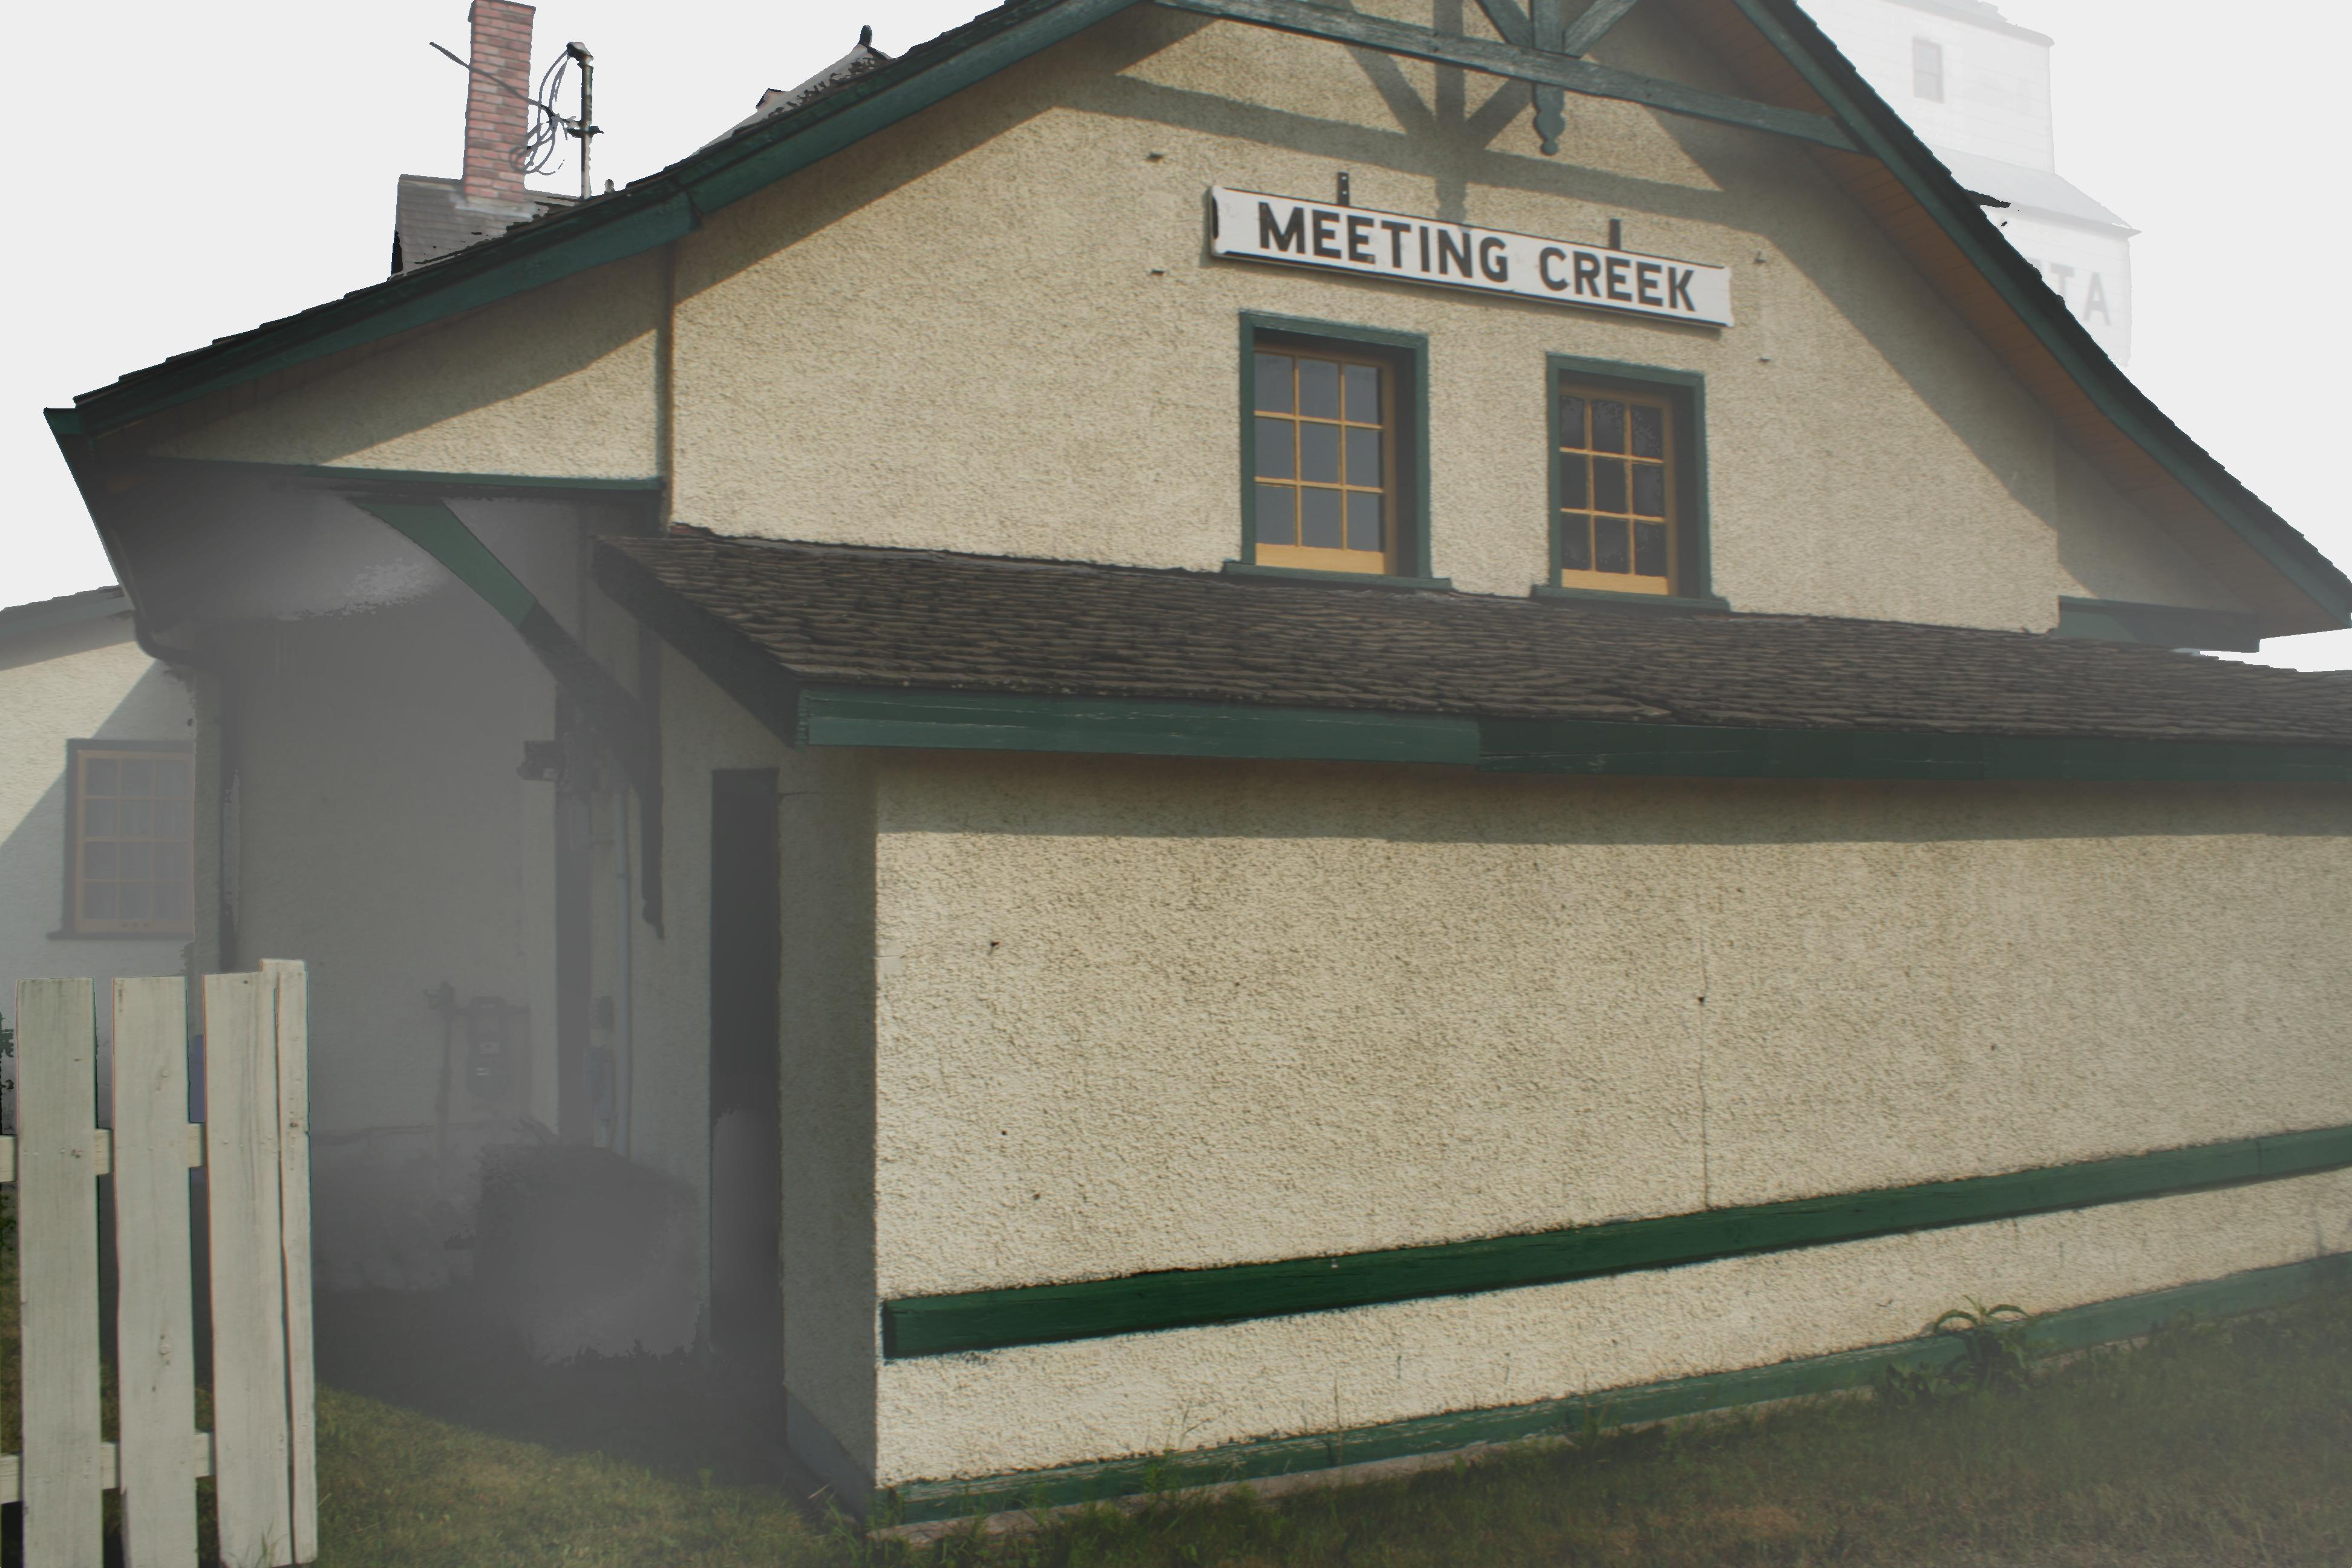
\includegraphics[width=5cm]{hazerd/img/dehaze_ren}}
  \subcaption{}
\end{subfigure}
\vfill
\caption{Example of algorithms' performances. (a): a haze free image from HazeRD, and the results of dehazing of a corresponding hazy image obtained with: (b):He~\cite{he2011single}, (c): Meng~\cite{meng2013efficient}, (d): Zhu~\cite{zhu2015fast}, (e): Berman~\cite{berman2016non}, (f): Cai~\cite{cai2016dehazenet}, and (g): Ren~\cite{Ren-ECCV-2016}.}
\label{fig:3.exmaple.hazerd}
\end{figure*}
\begin{figure*}[htb]
\begin{subfigure}[b]{1\linewidth}
  \centering
  \centerline{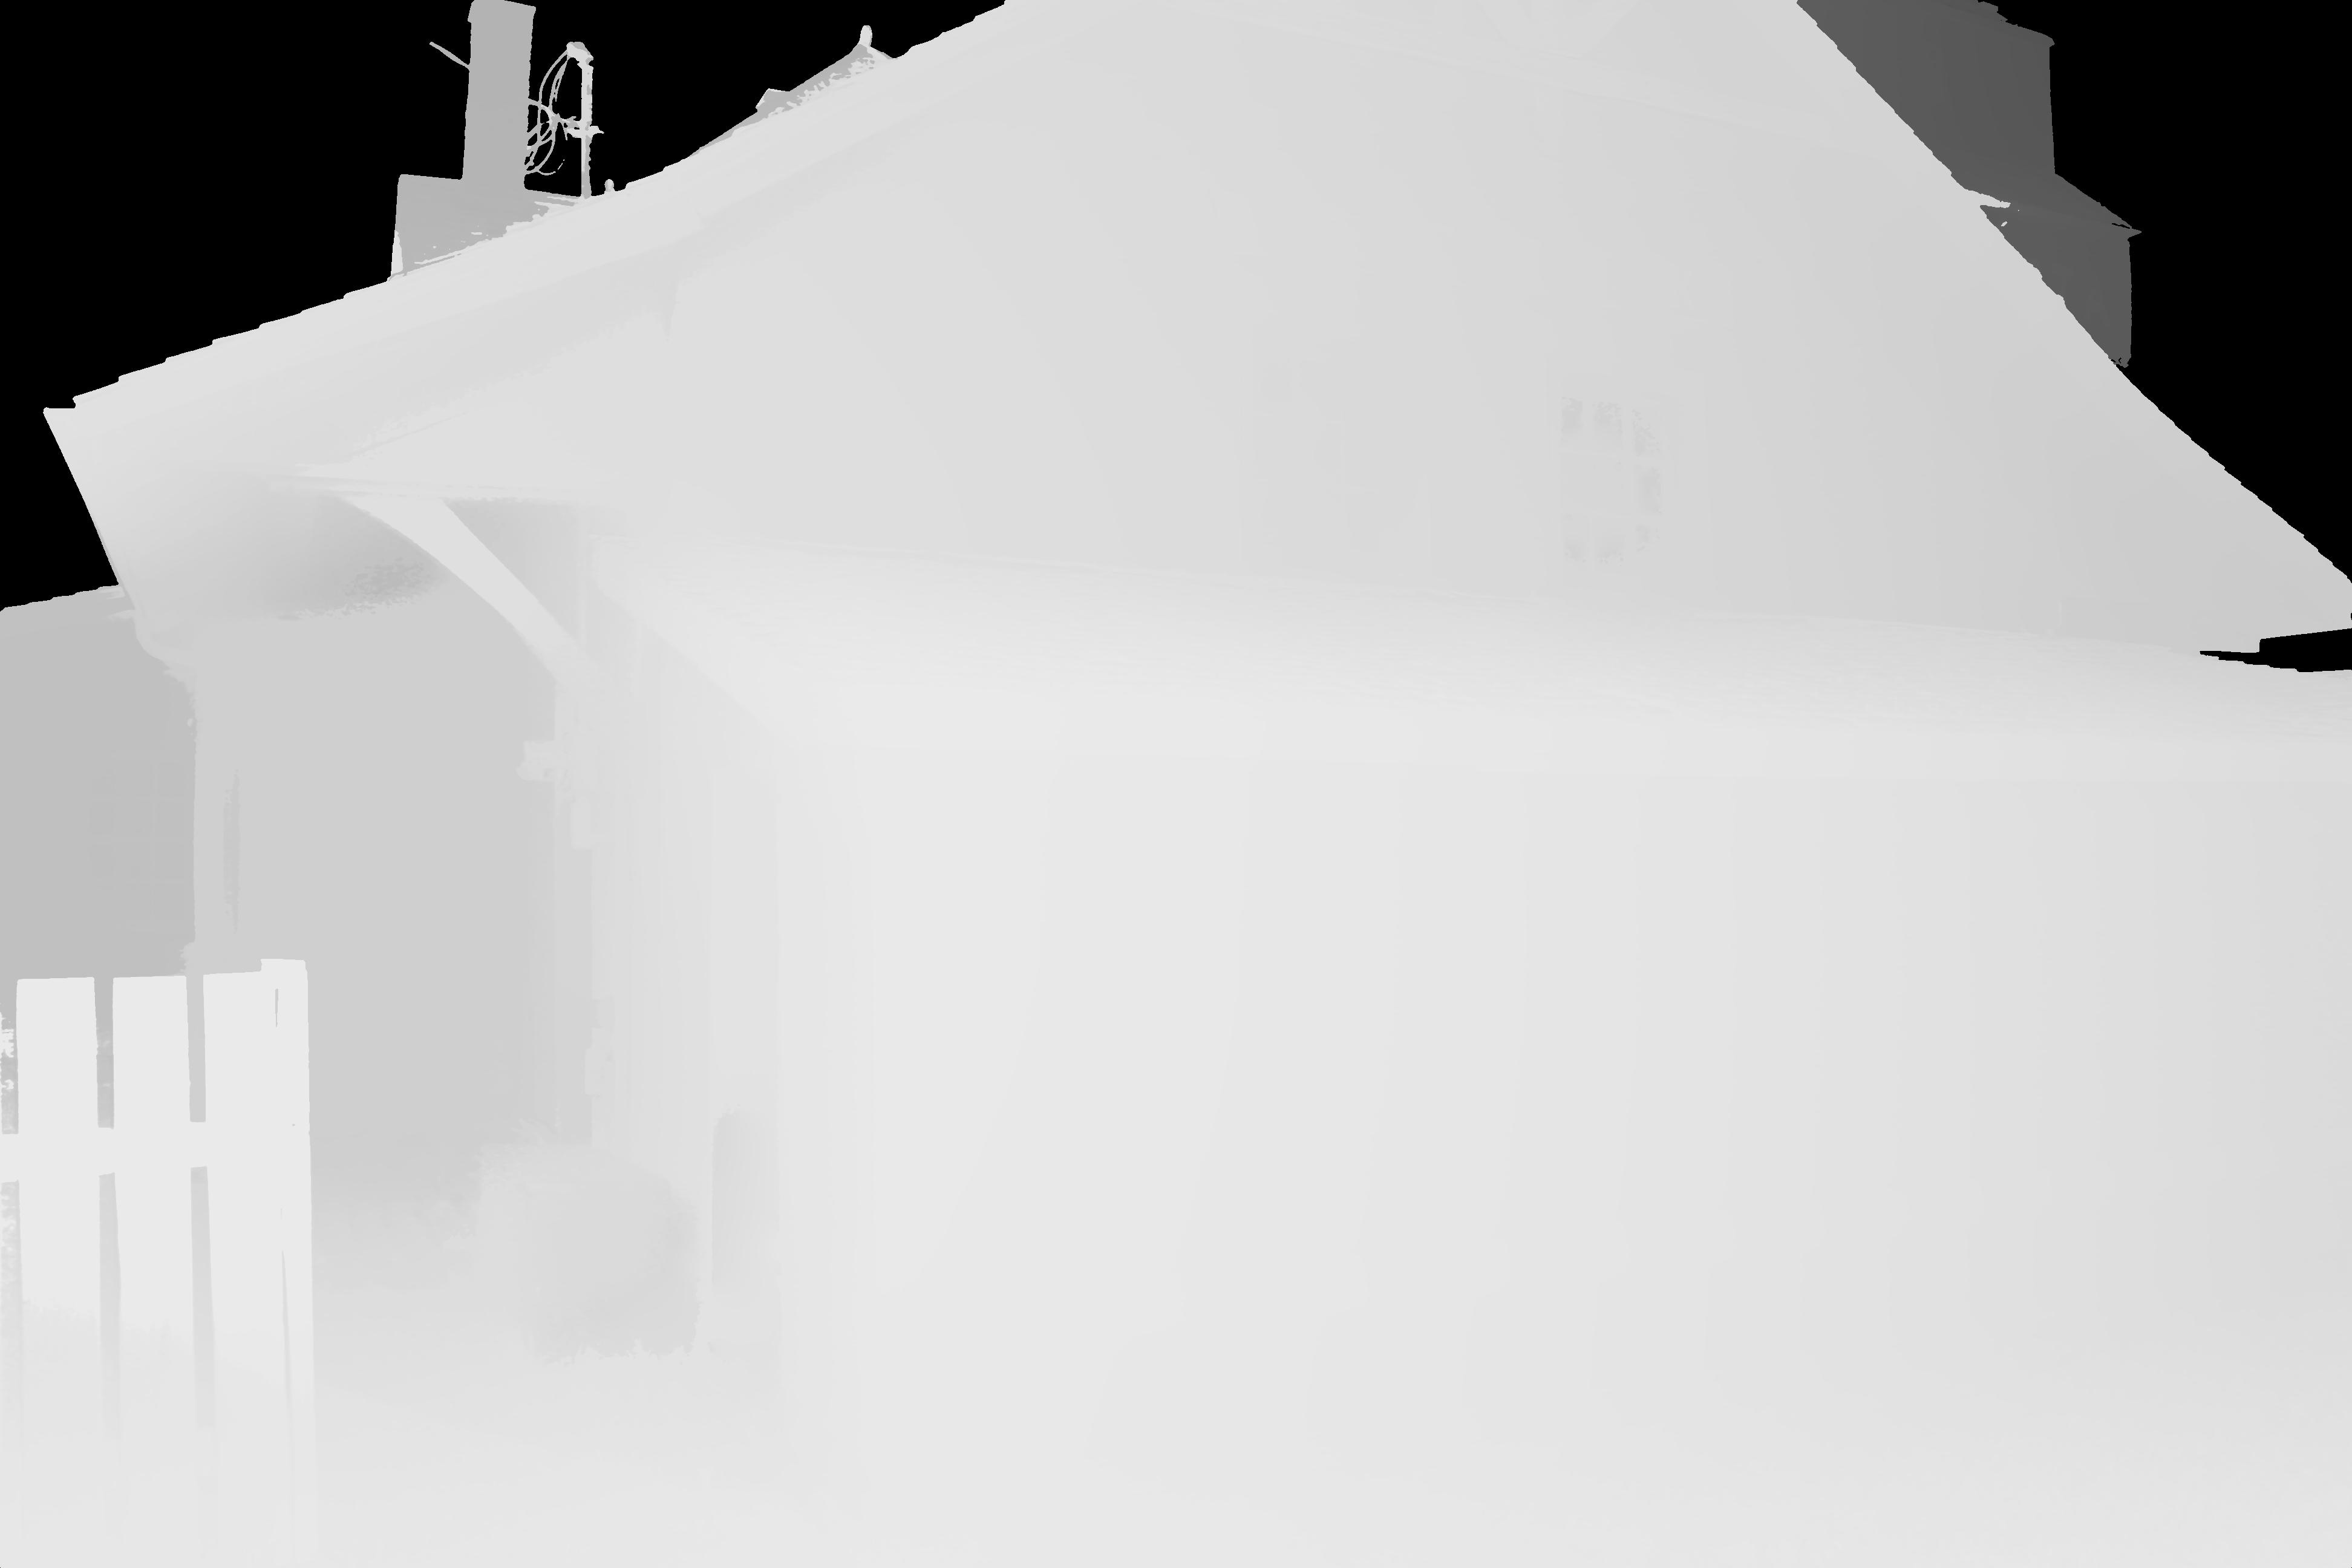
\includegraphics[width=6cm]{hazerd/img/ori}}
  \subcaption{}
\end{subfigure}
\vfill
\begin{subfigure}[b]{0.45\linewidth}
  \centering
  \centerline{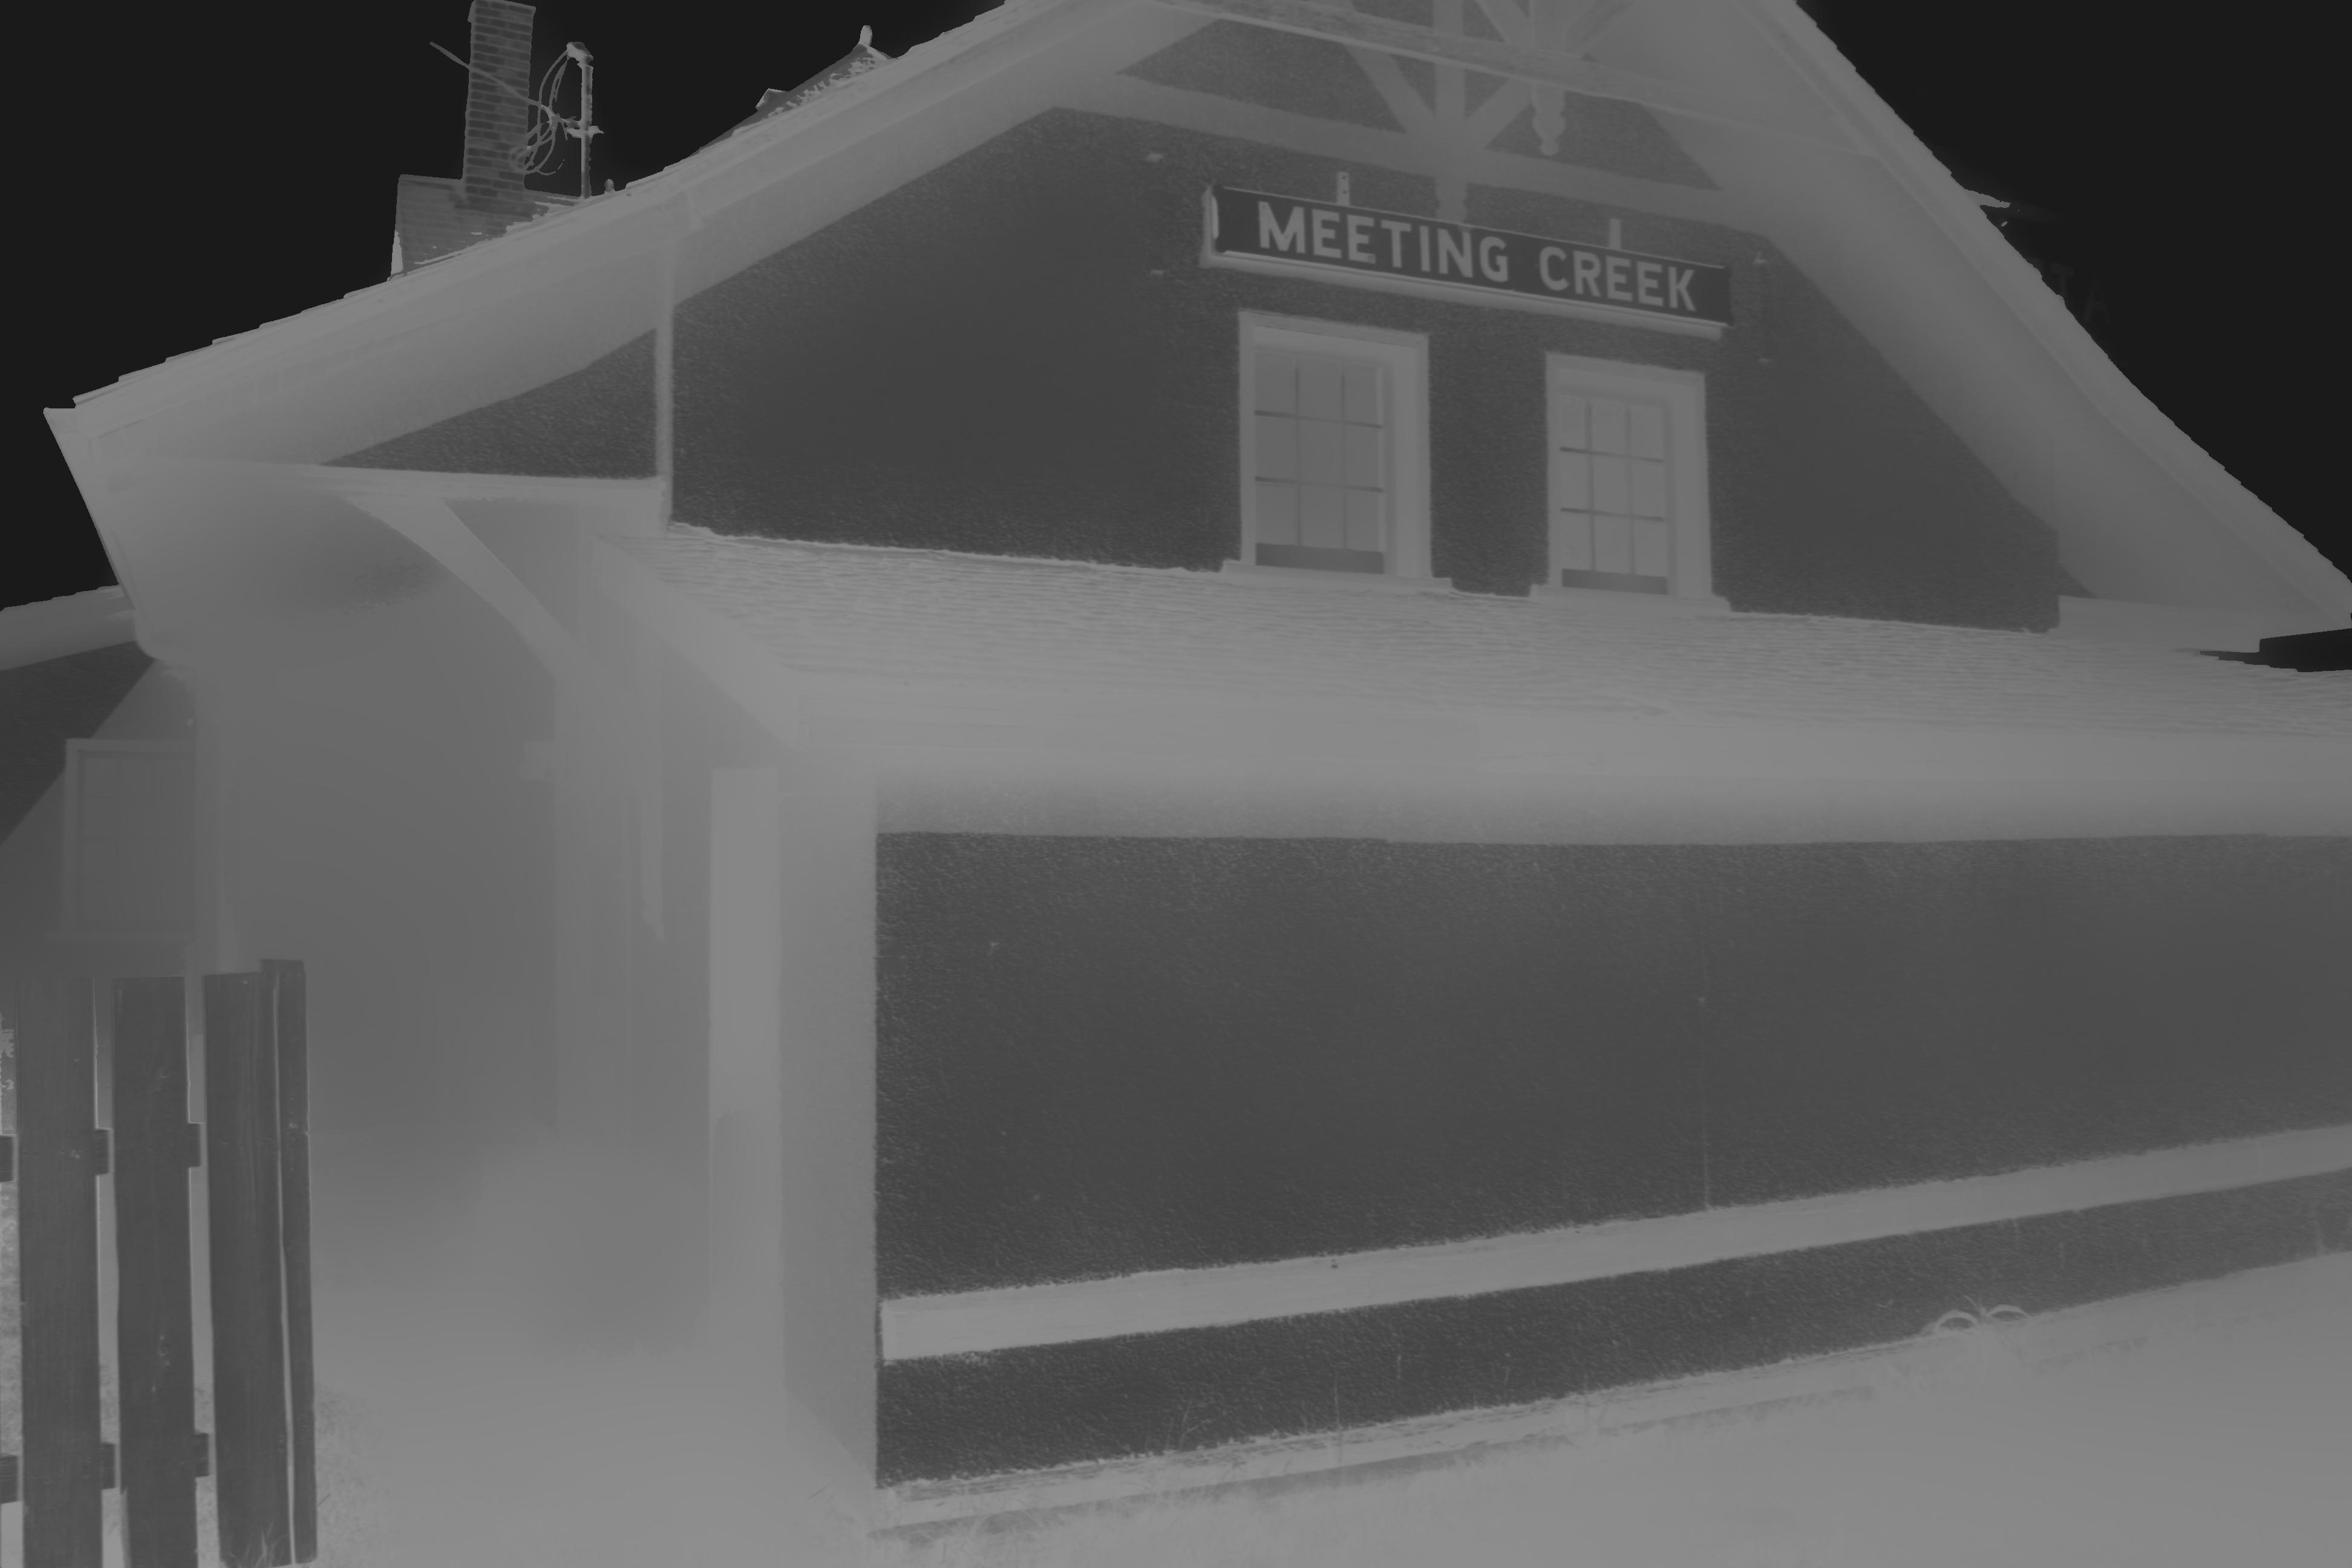
\includegraphics[width=5cm]{hazerd/img/he}}
  \subcaption{}
\end{subfigure}
\hfill
\begin{subfigure}[b]{0.45\linewidth}
  \centering
  \centerline{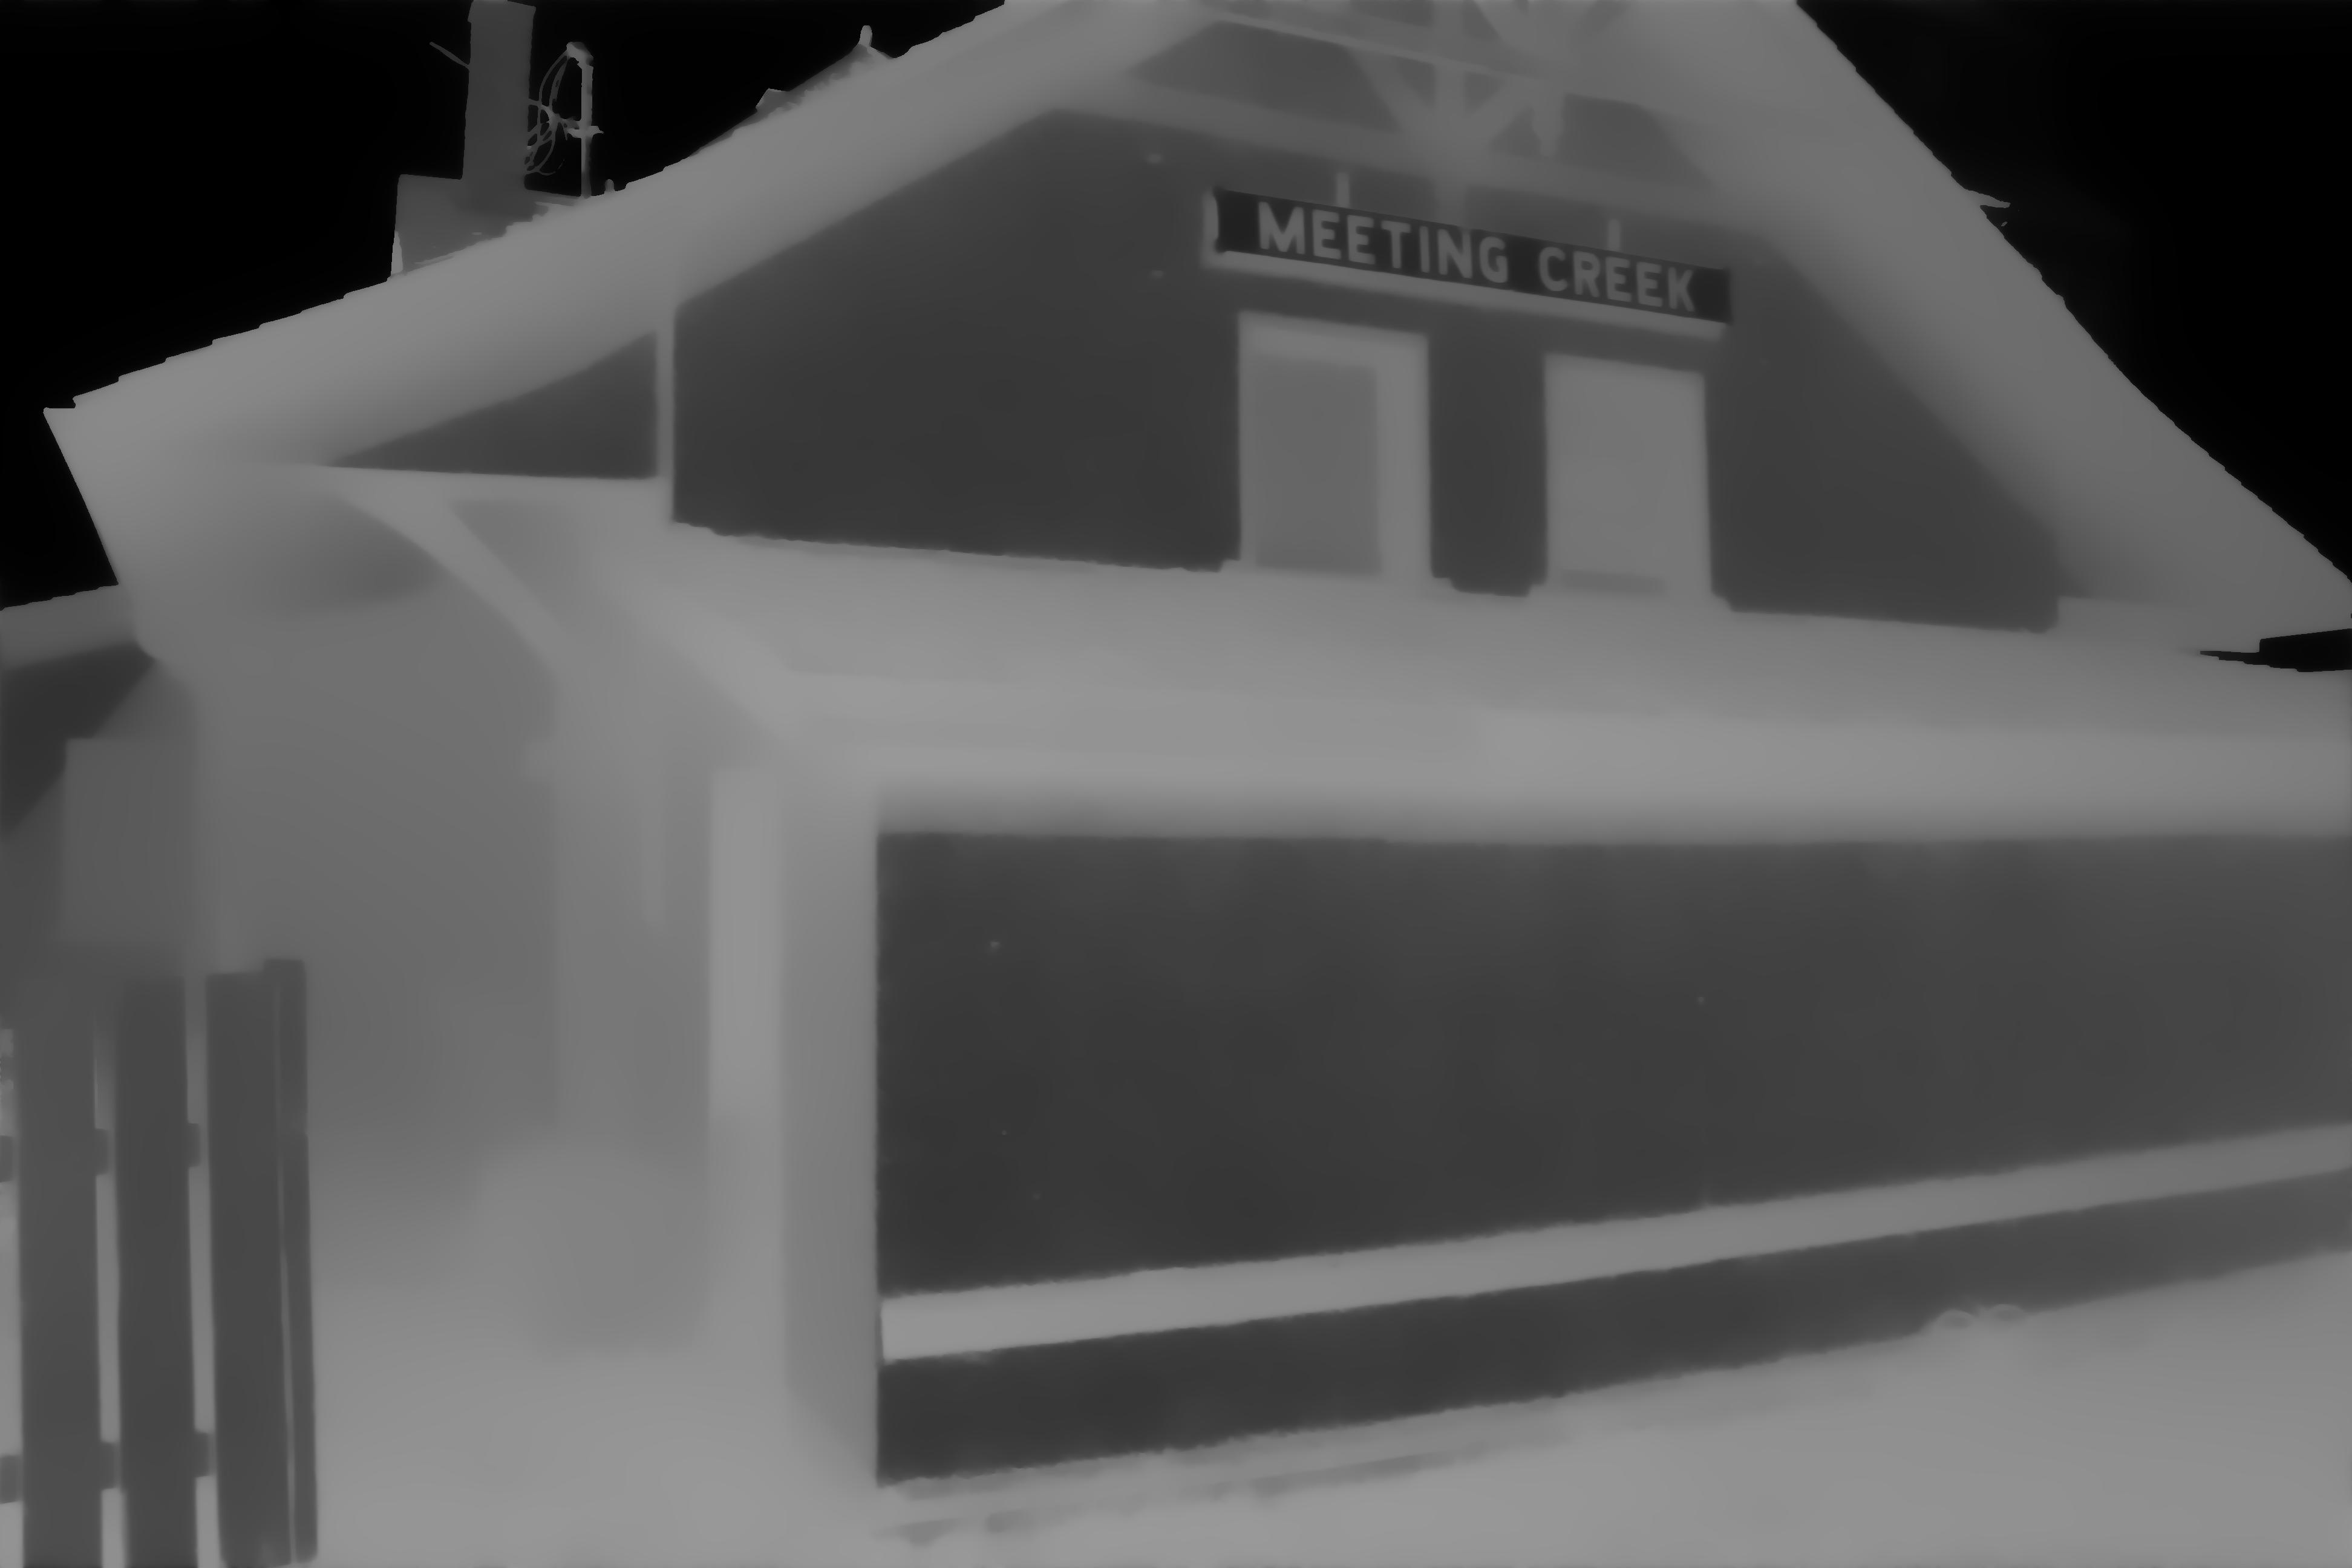
\includegraphics[width=5cm]{hazerd/img/meng}}
  \subcaption{}
\end{subfigure}
\vfill
\begin{subfigure}[b]{0.45\linewidth}
  \centering
  \centerline{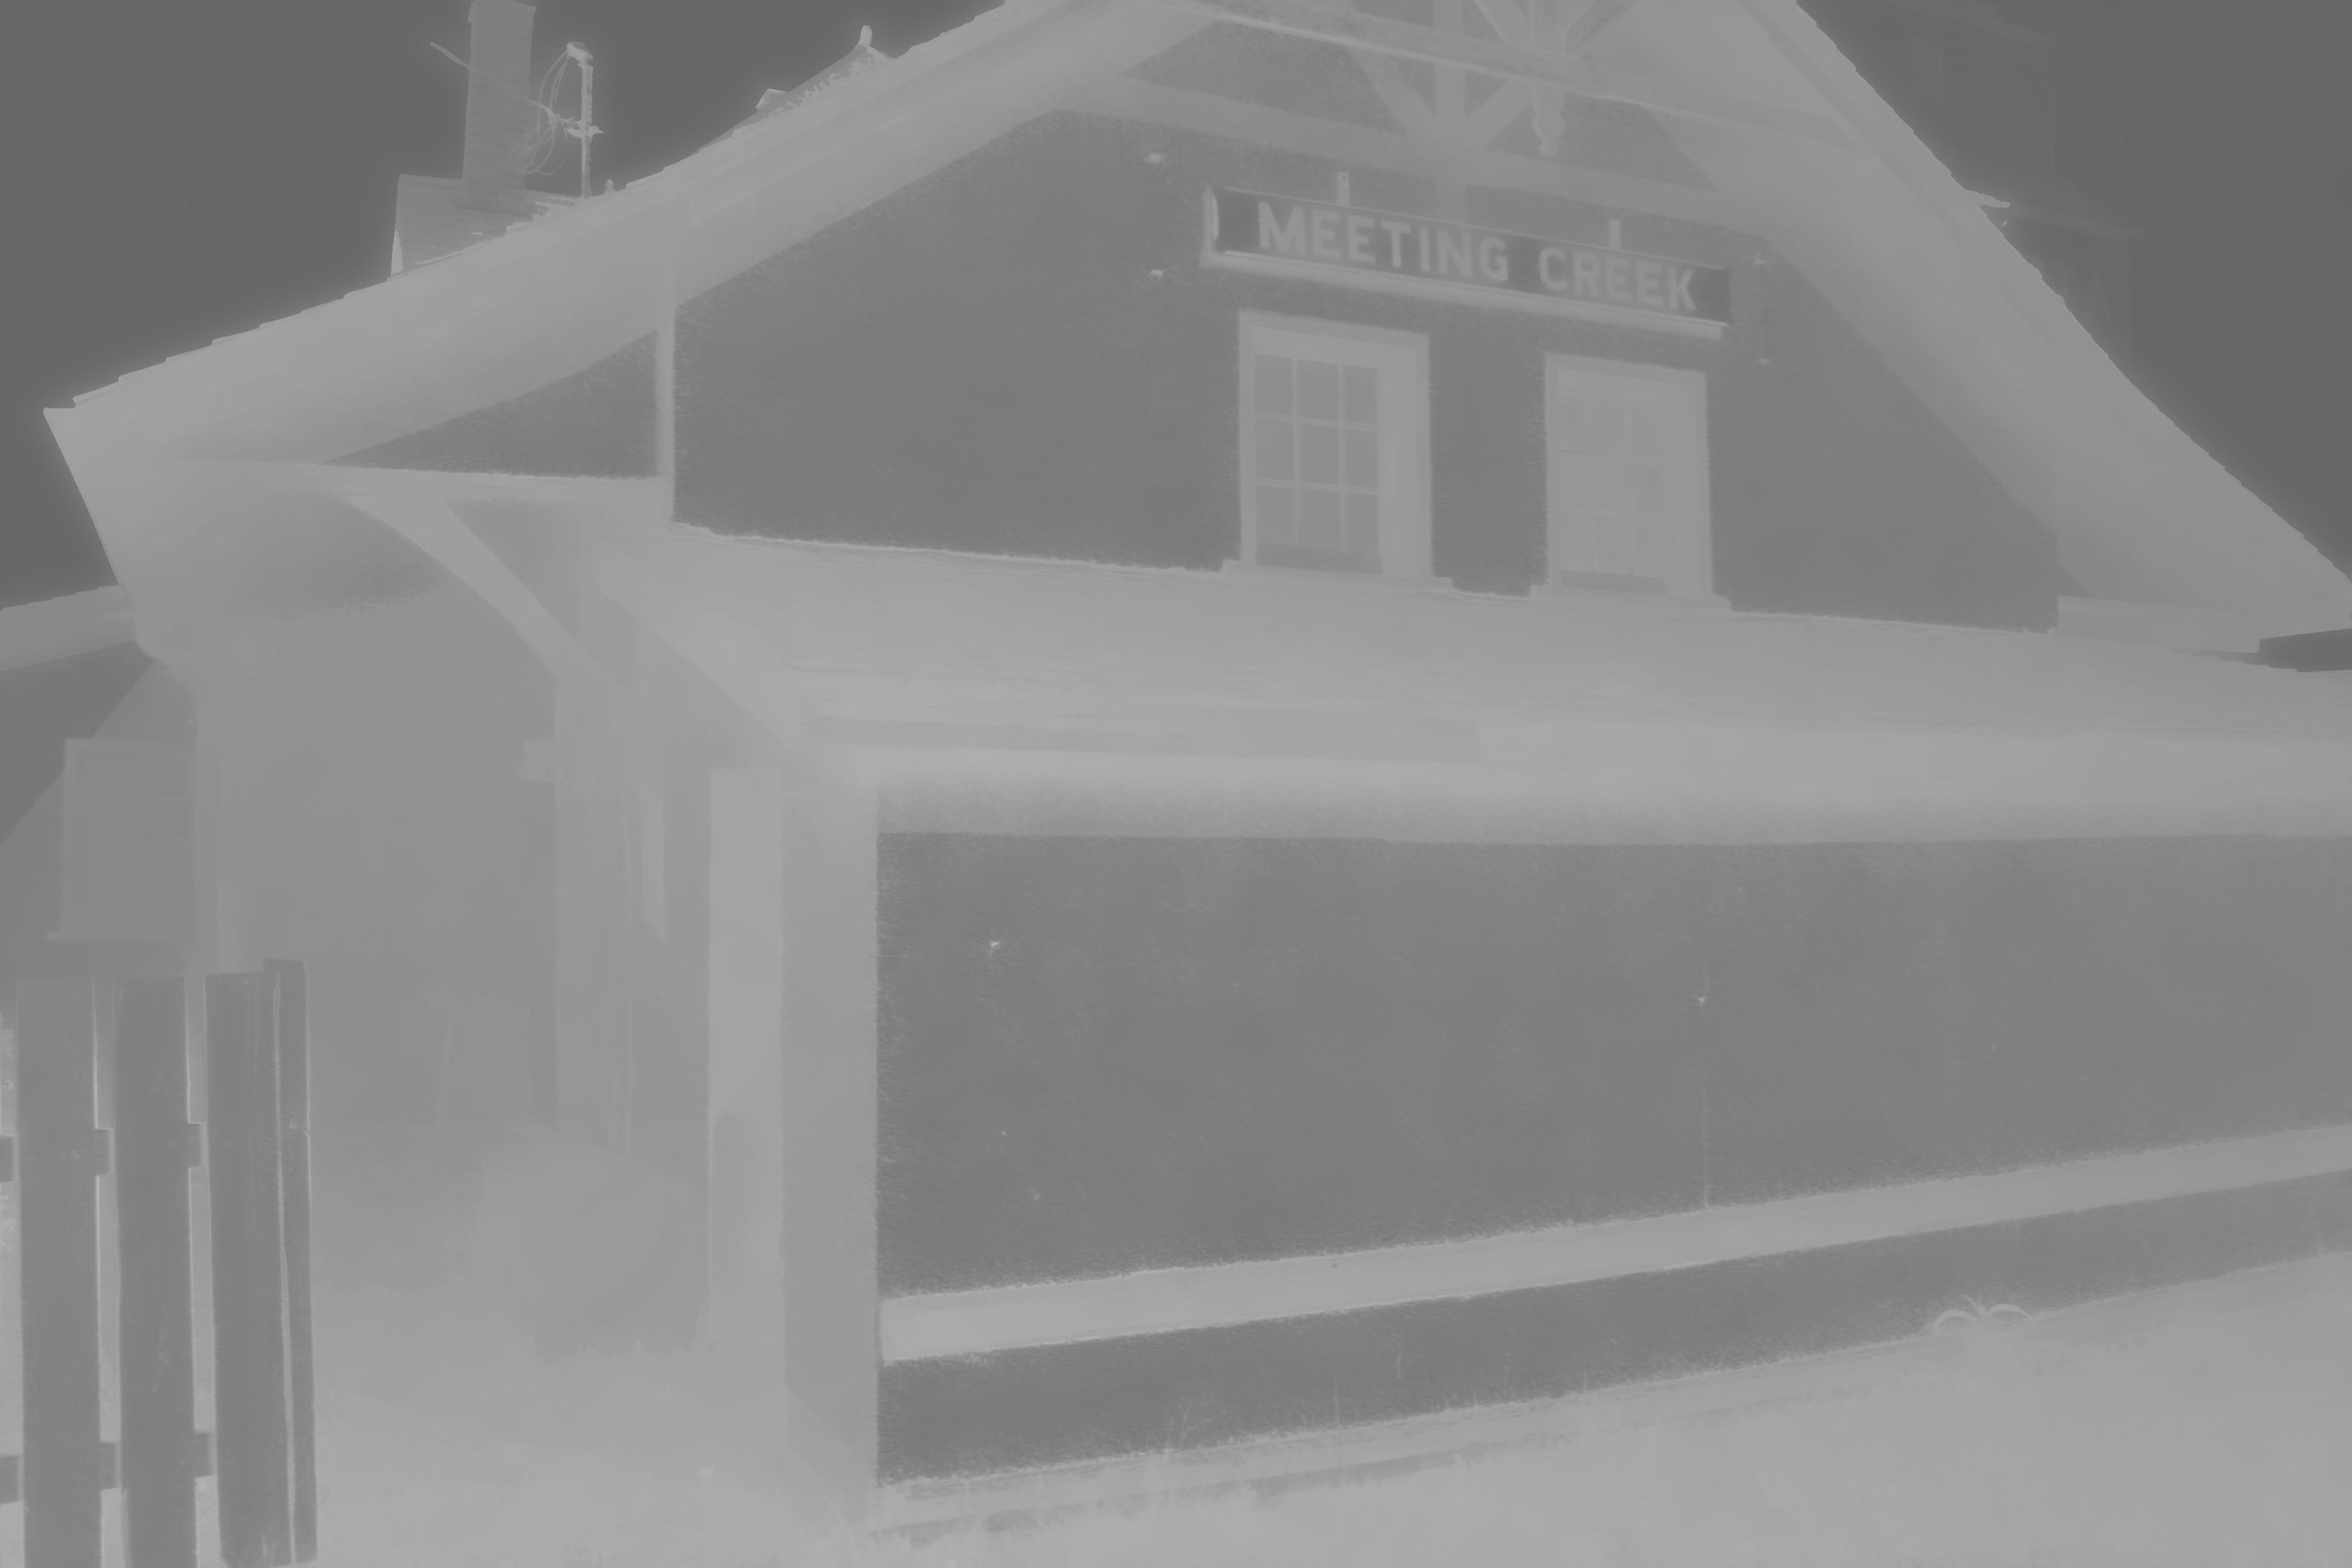
\includegraphics[width=5cm]{hazerd/img/zhu}}
  \subcaption{}
\end{subfigure}
\hfill
\begin{subfigure}[b]{0.45\linewidth}
  \centering
  \centerline{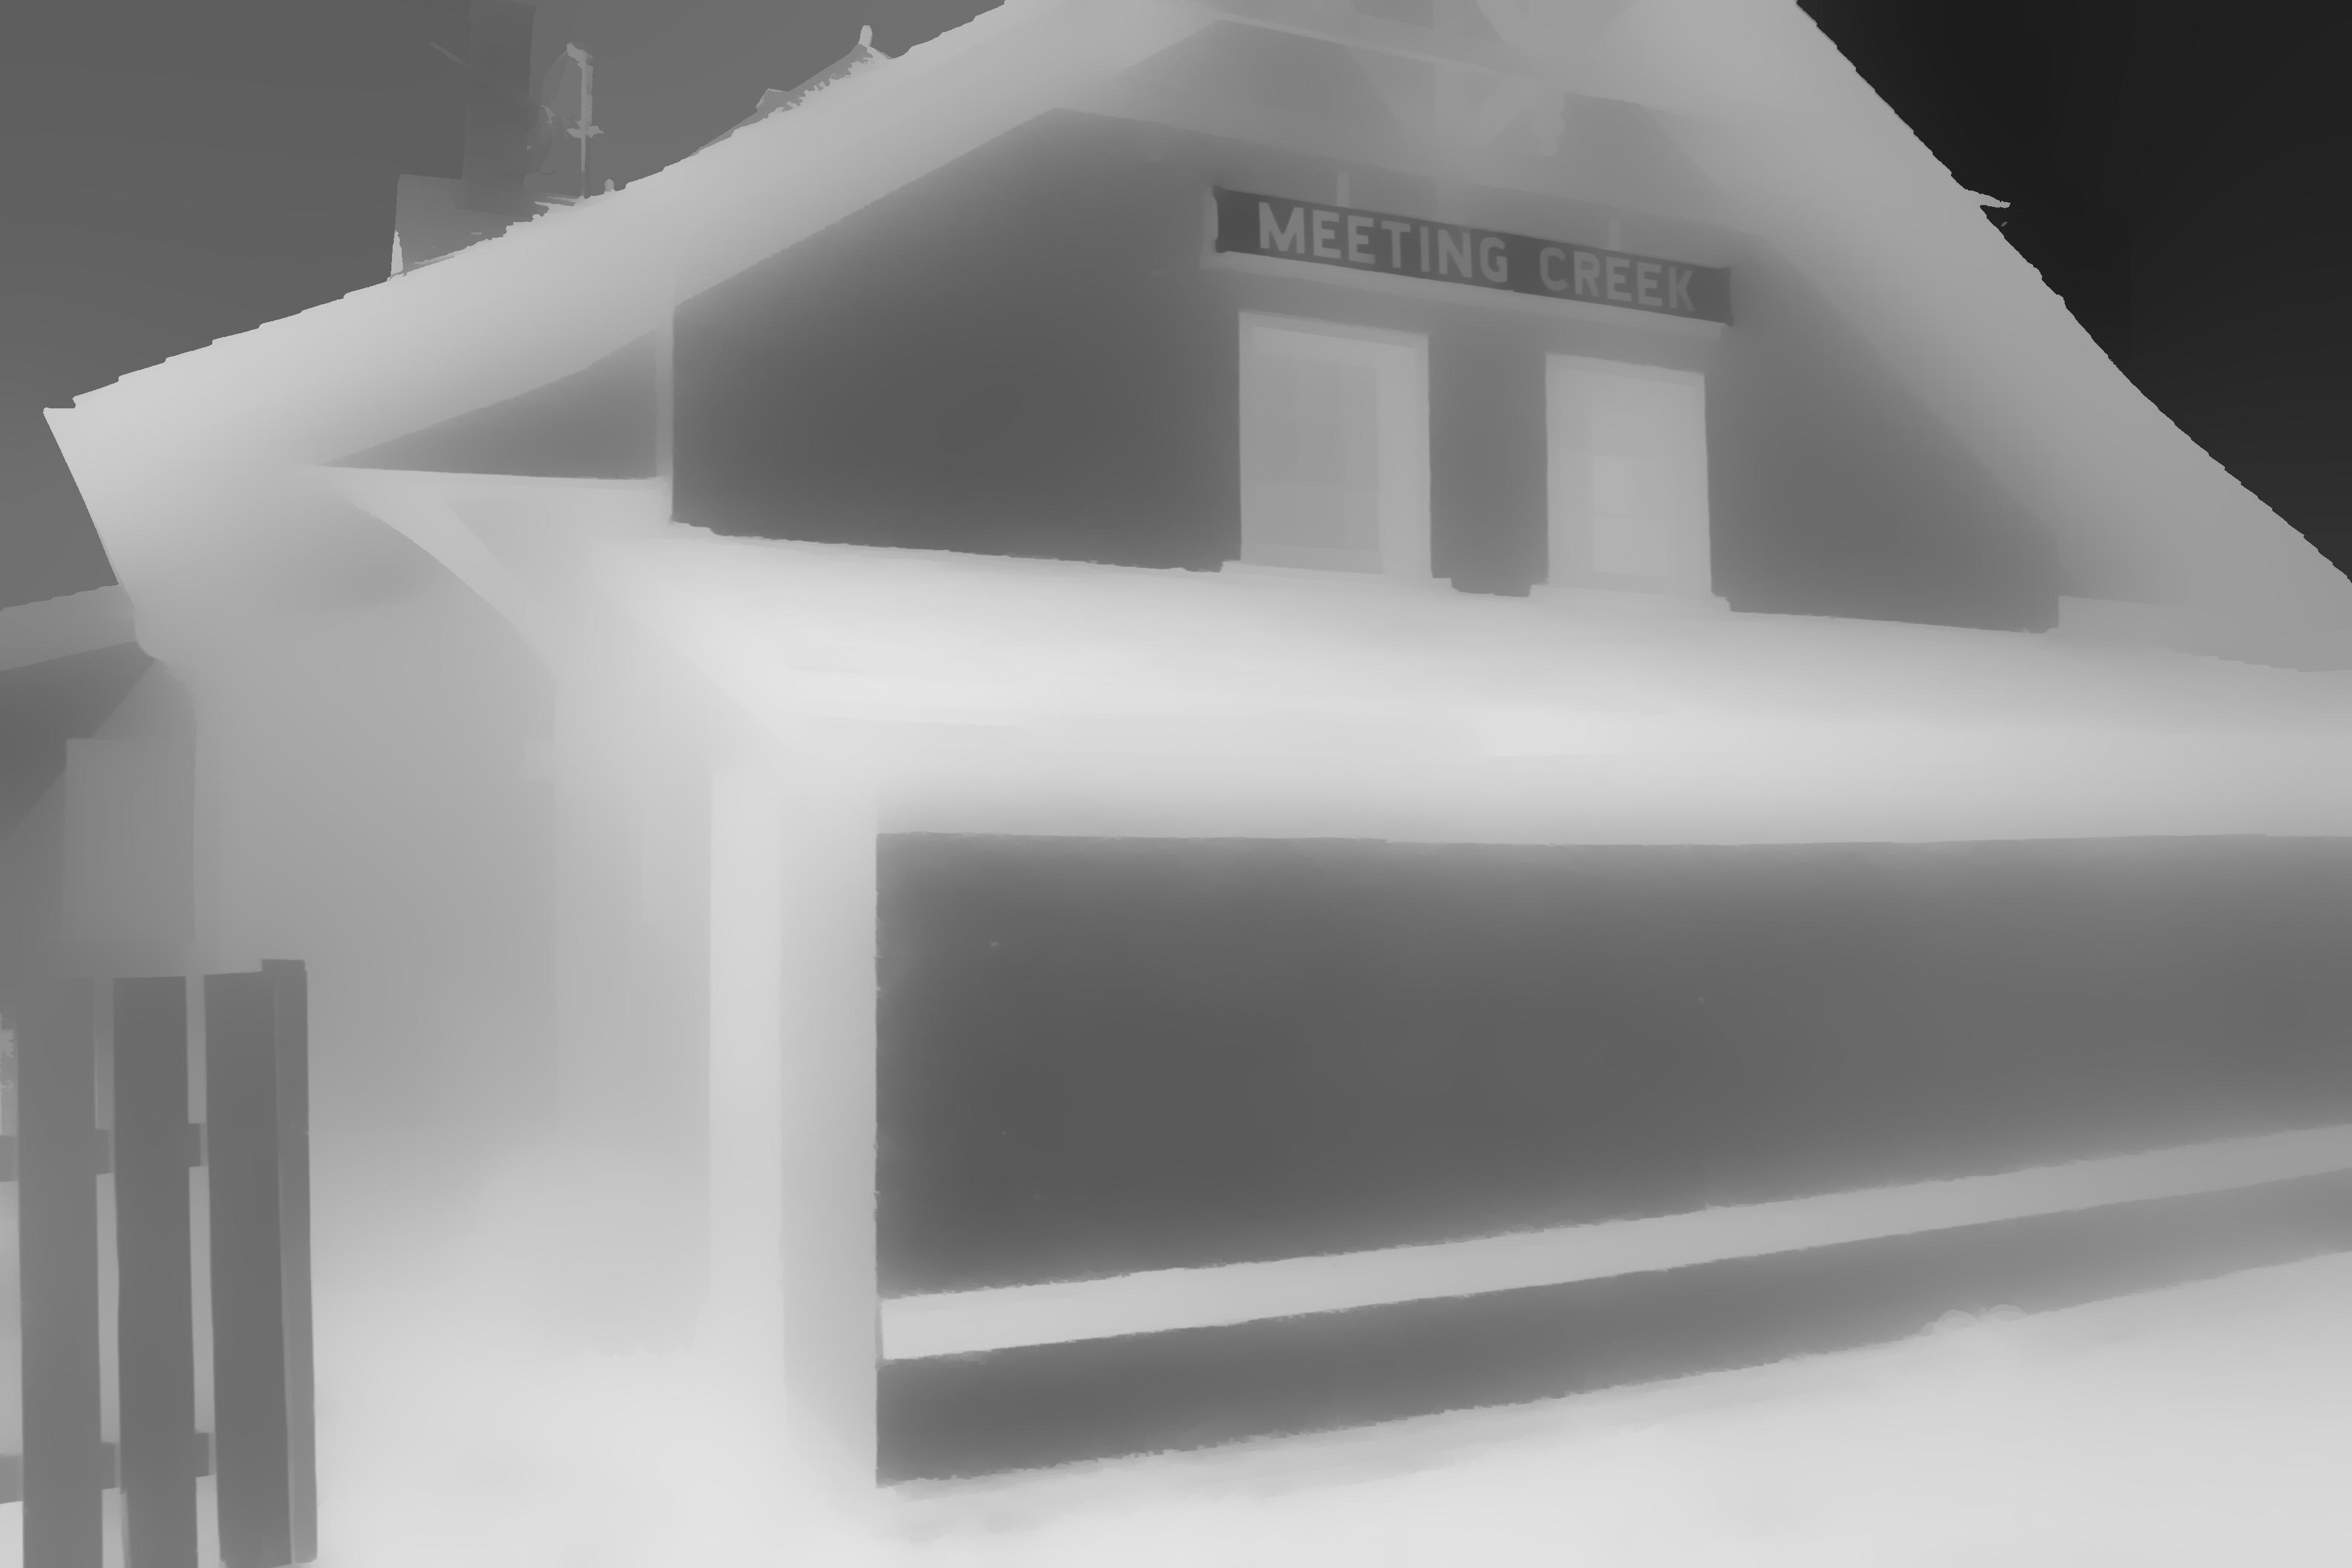
\includegraphics[width=5cm]{hazerd/img/berman}}
  \subcaption{}
\end{subfigure}
\vfill
\begin{subfigure}[b]{0.45\linewidth}
  \centering
  \centerline{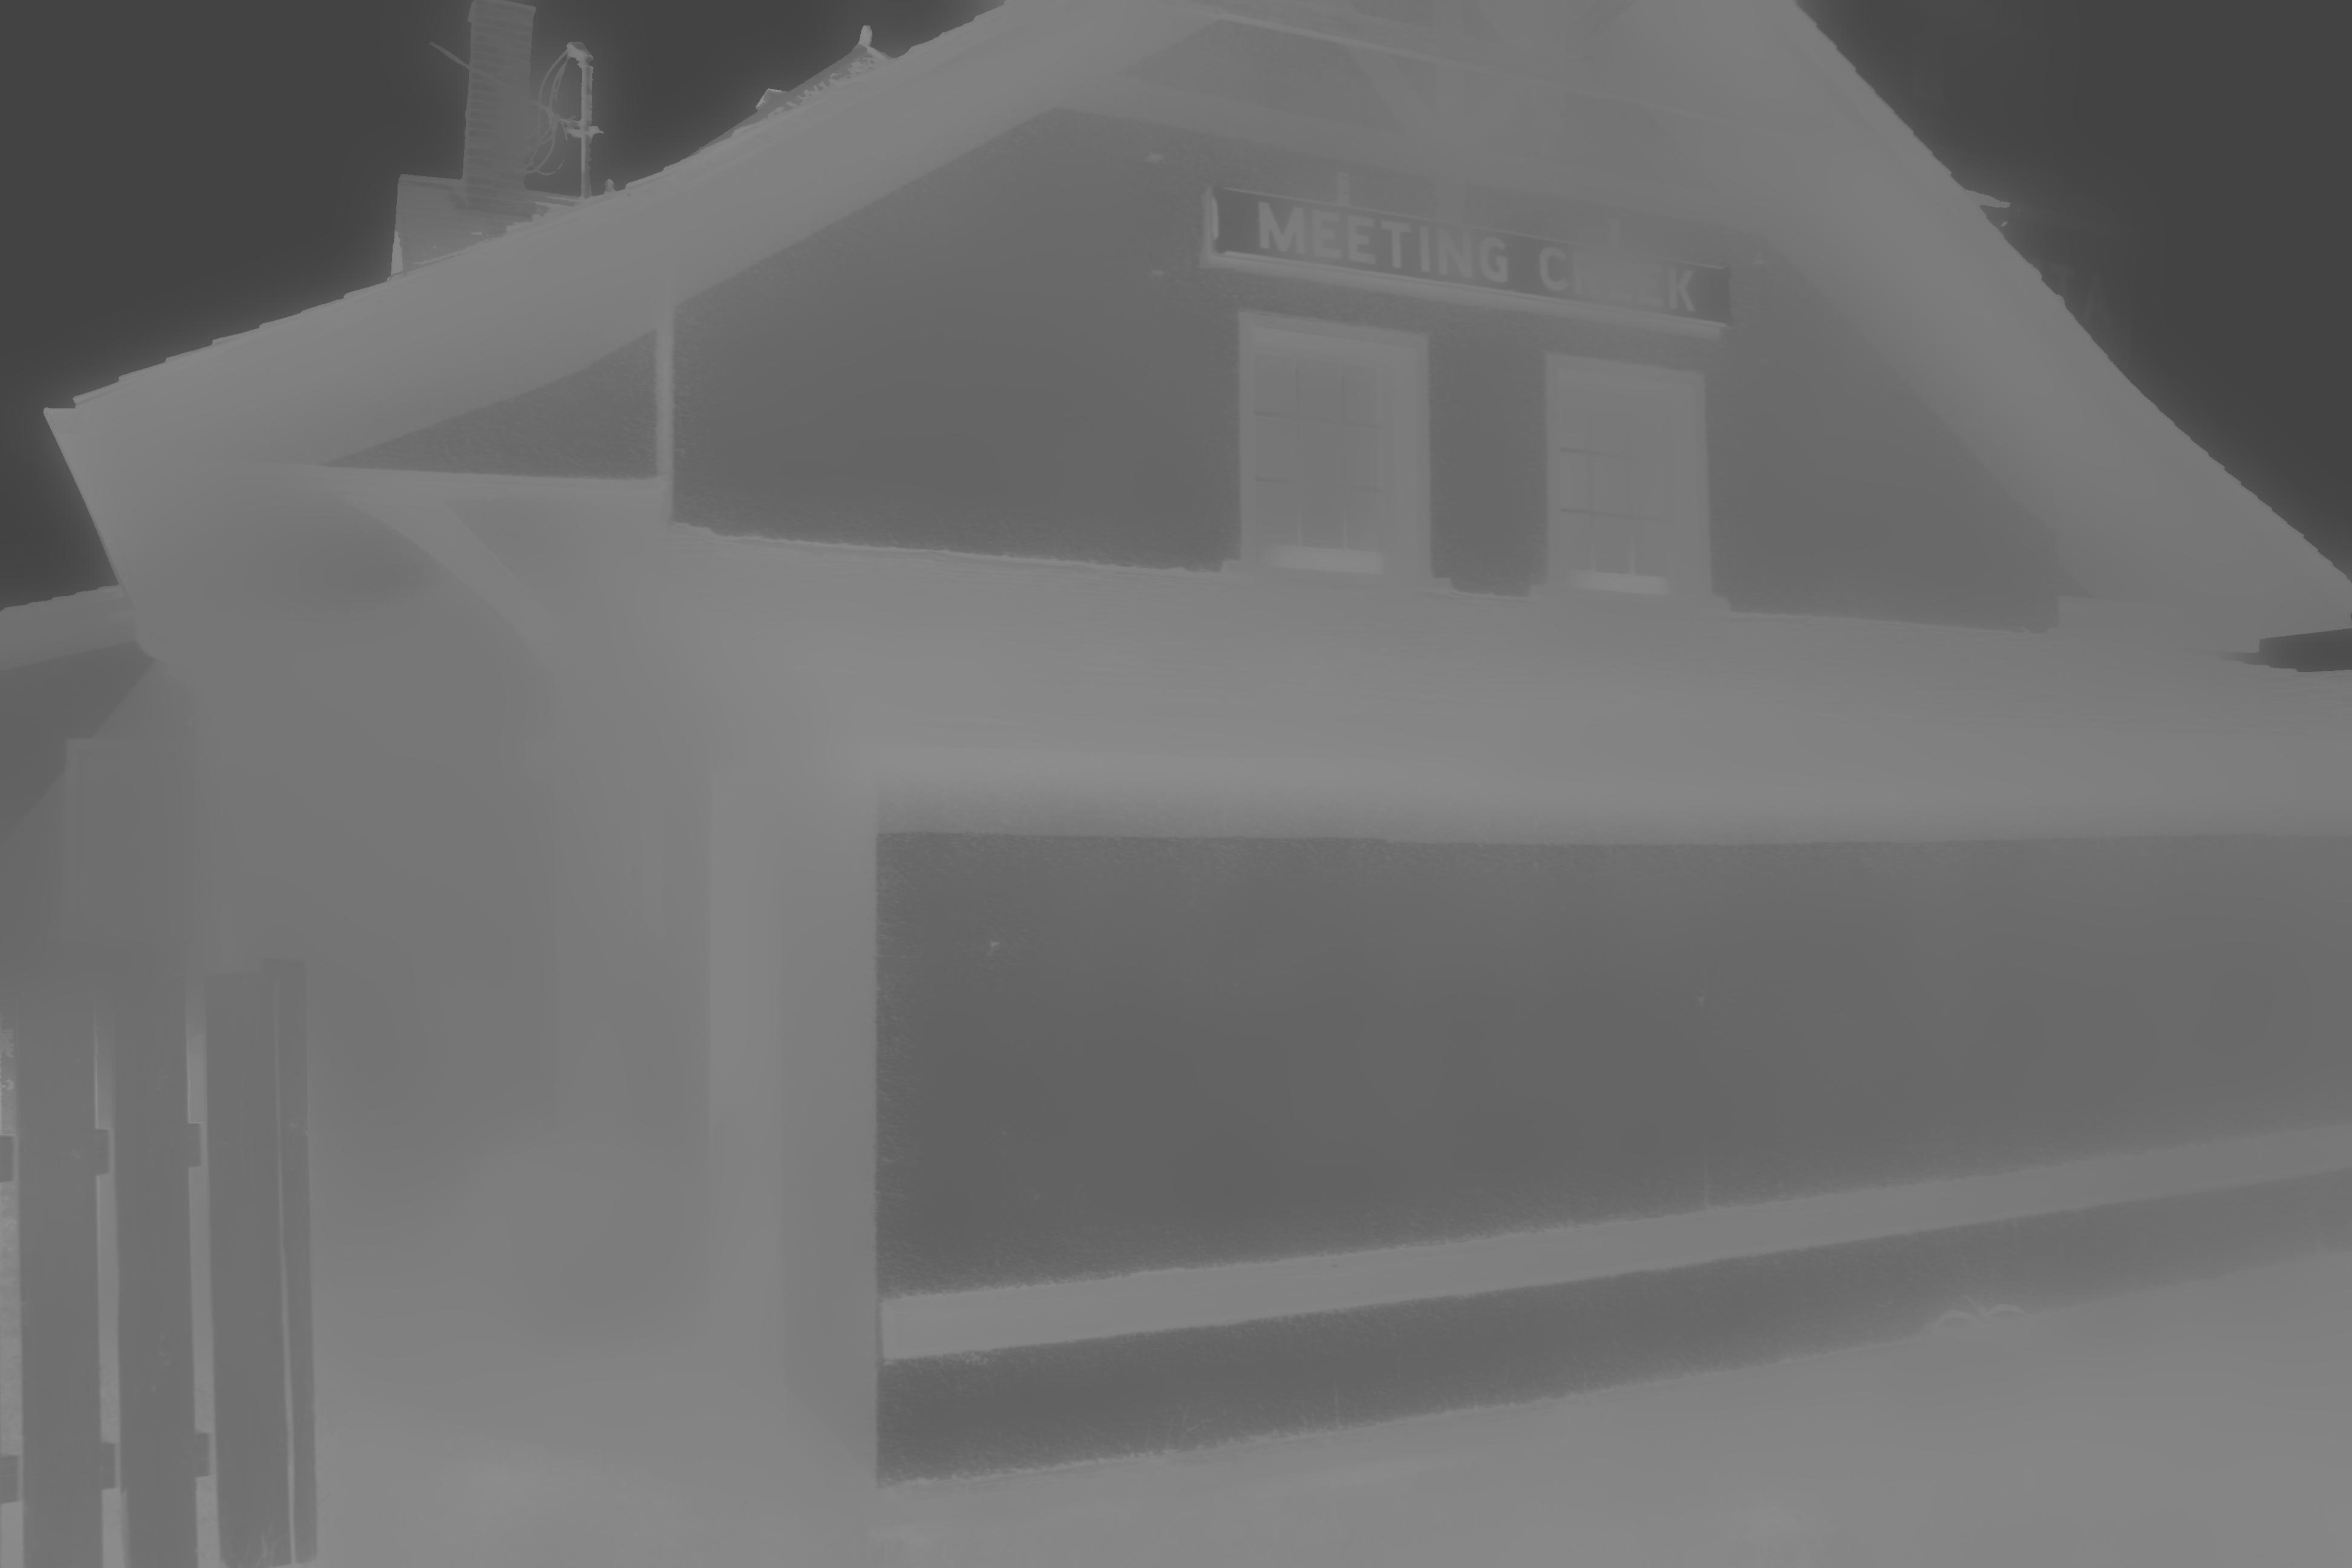
\includegraphics[width=5cm]{hazerd/img/cai}}
  \subcaption{}
\end{subfigure}
\hfill
\begin{subfigure}[b]{0.45\linewidth}
  \centering
  \centerline{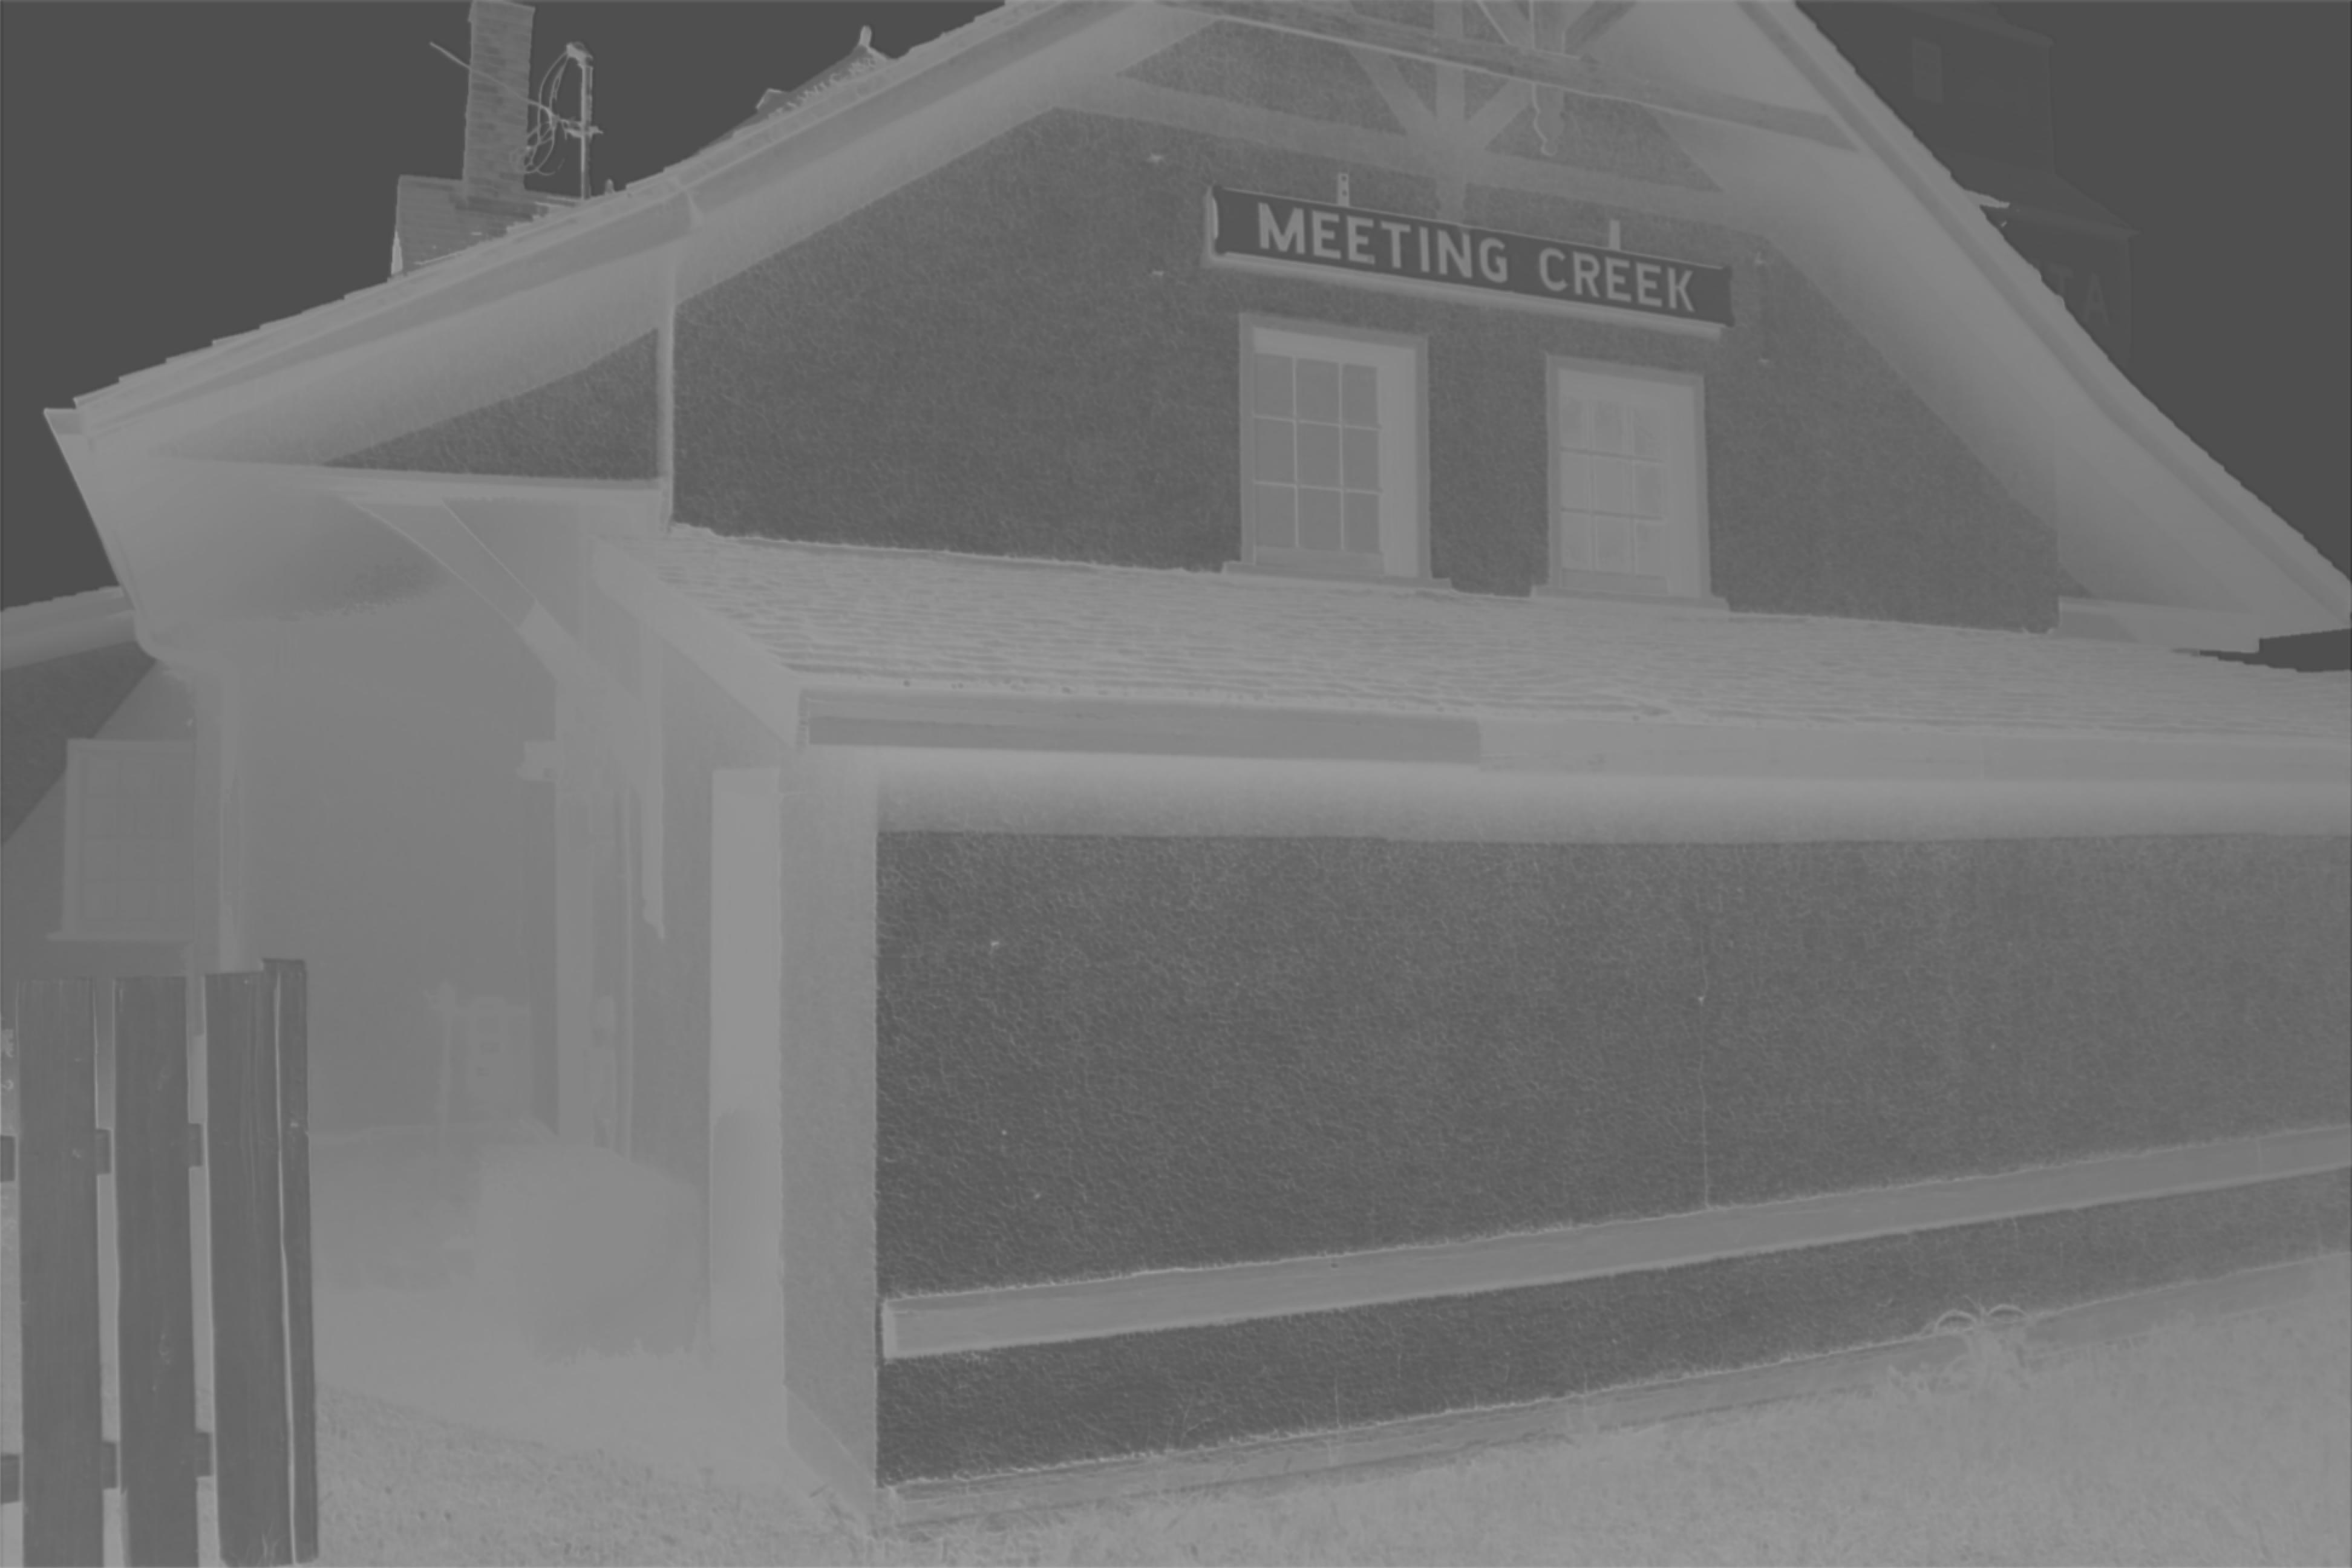
\includegraphics[width=5cm]{hazerd/img/ren}}
  \subcaption{}
\end{subfigure}
\vfill
\caption{Example of algorithms' performances. (a): the ground truth transmission for the haze free image in~\ref{fig:3.exmaple.hazerd}, and the transmission estimates corresponding to the estimated images obtained with: (b):He~\cite{he2011single}, (c): Meng~\cite{meng2013efficient}, (d): Zhu~\cite{zhu2015fast}, (e): Berman~\cite{berman2016non}, (f): Cai~\cite{cai2016dehazenet}, and (g): Ren~\cite{Ren-ECCV-2016}.}
\label{fig:3.exmaple.hazerd.trans}
\end{figure*}
\begin{figure*}[htb]
\begin{subfigure}[b]{1\linewidth}
  \centering
  \centerline{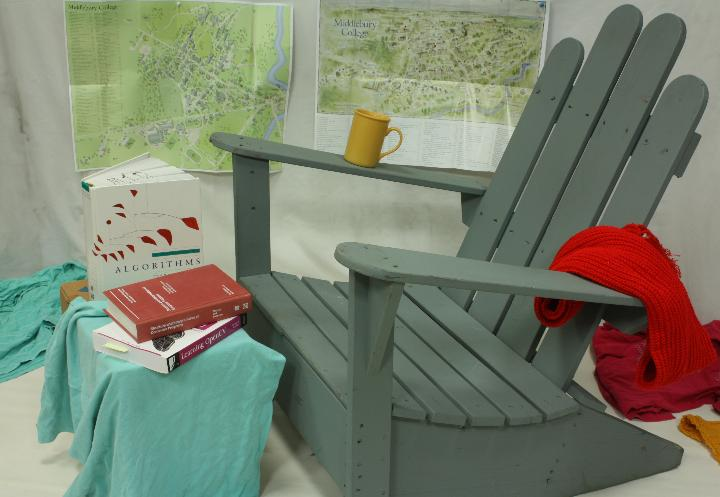
\includegraphics[width=6cm]{hazerd/middlebury/ori}}
  \subcaption{}
\end{subfigure}
\vfill
\begin{subfigure}[b]{0.45\linewidth}
  \centering
  \centerline{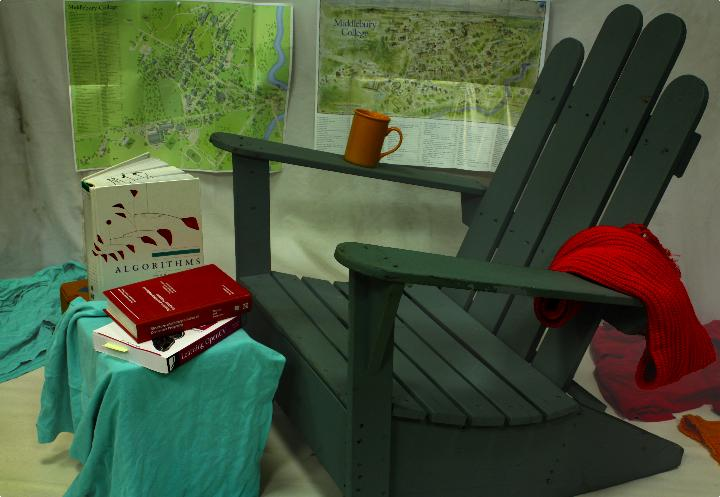
\includegraphics[width=5cm]{hazerd/middlebury/dehaze_he}}
  \subcaption{}
\end{subfigure}
\hfill
\begin{subfigure}[b]{0.45\linewidth}
  \centering
  \centerline{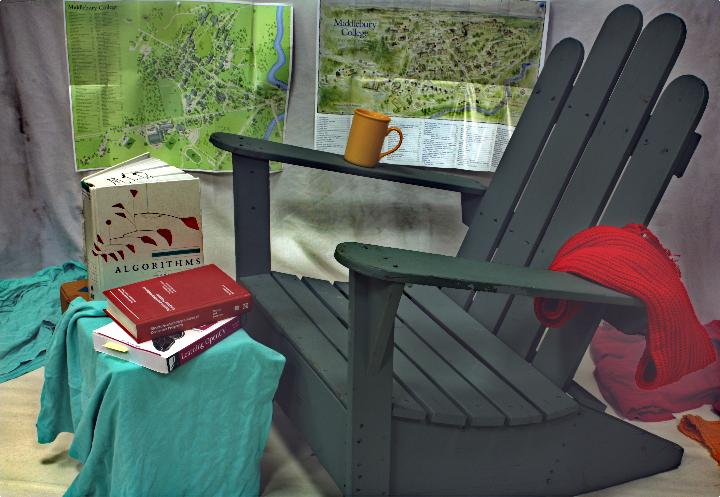
\includegraphics[width=5cm]{hazerd/middlebury/dehaze_meng}}
  \subcaption{}
\end{subfigure}
\vfill
\begin{subfigure}[b]{0.45\linewidth}
  \centering
  \centerline{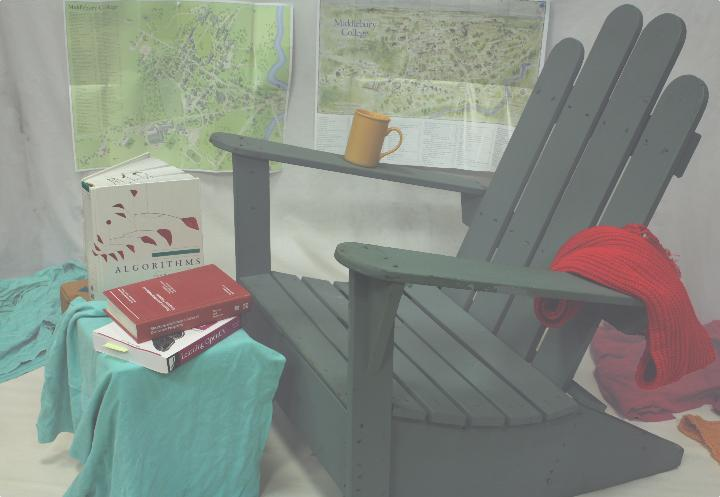
\includegraphics[width=5cm]{hazerd/middlebury/dehaze_zhu}}
  \subcaption{}
\end{subfigure}
\hfill
\begin{subfigure}[b]{0.45\linewidth}
  \centering
  \centerline{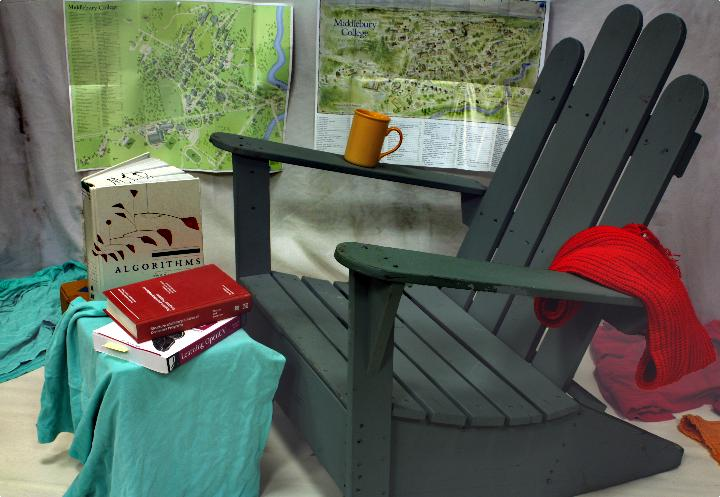
\includegraphics[width=5cm]{hazerd/middlebury/dehaze_berman}}
  \subcaption{}
\end{subfigure}
\vfill
\begin{subfigure}[b]{0.45\linewidth}
  \centering
  \centerline{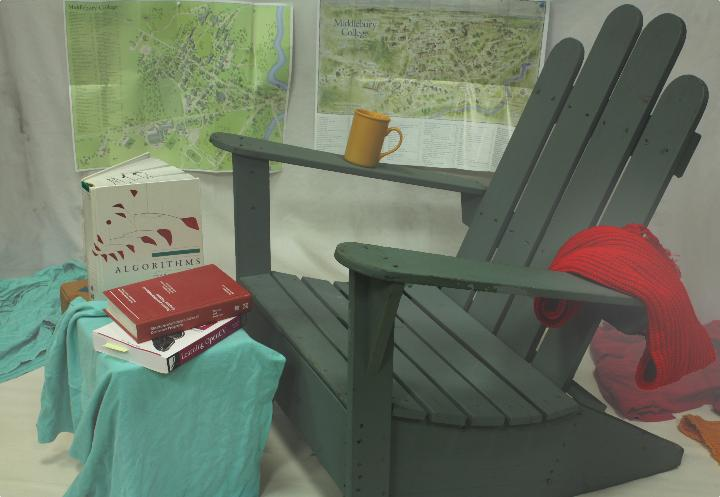
\includegraphics[width=5cm]{hazerd/middlebury/dehaze_cai}}
  \subcaption{}
\end{subfigure}
\hfill
\begin{subfigure}[b]{0.45\linewidth}
  \centering
  \centerline{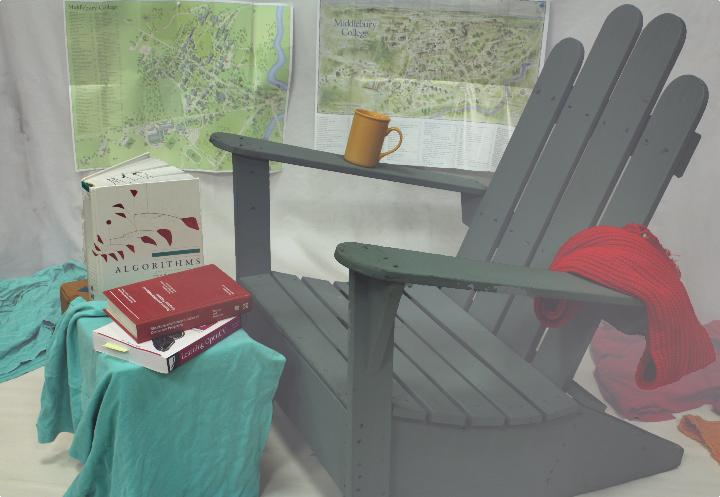
\includegraphics[width=5cm]{hazerd/middlebury/dehaze_ren}}
  \subcaption{}
\end{subfigure}
\vfill
\caption{Example of algorithms' performances. (a): a haze free image from Middlebury dataset, and the results of dehazing of a corresponding hazy image obtained with: (b):He~\cite{he2011single}, (c): Meng~\cite{meng2013efficient}, (d): Zhu~\cite{zhu2015fast}, (e): Berman~\cite{berman2016non}, (f): Cai~\cite{cai2016dehazenet}, and (g): Ren~\cite{Ren-ECCV-2016}.}
\label{fig:3.exmaple.middlebury}
\end{figure*}
\begin{figure*}[htb]
\begin{subfigure}[b]{1\linewidth}
  \centering
  \centerline{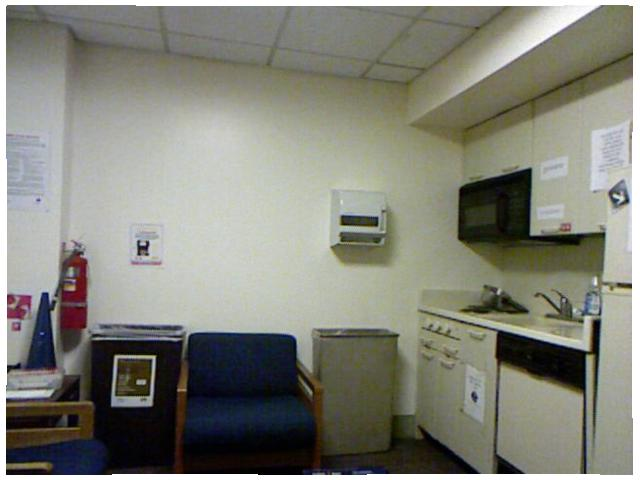
\includegraphics[width=6cm]{hazerd/nyu/ori}}
  \subcaption{}
\end{subfigure}
\vfill
\begin{subfigure}[b]{0.45\linewidth}
  \centering
  \centerline{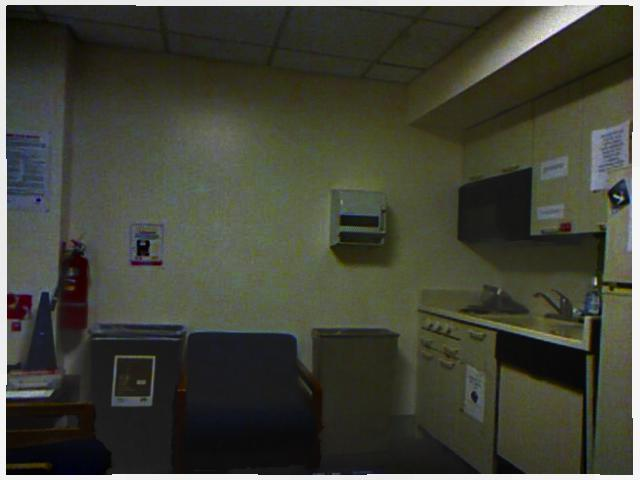
\includegraphics[width=5cm]{hazerd/nyu/dehaze_he}}
  \subcaption{}
\end{subfigure}
\hfill
\begin{subfigure}[b]{0.45\linewidth}
  \centering
  \centerline{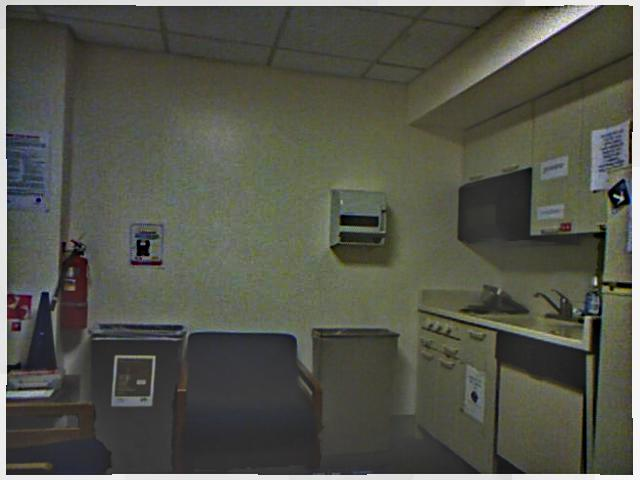
\includegraphics[width=5cm]{hazerd/nyu/dehaze_meng}}
  \subcaption{}
\end{subfigure}
\vfill
\begin{subfigure}[b]{0.45\linewidth}
  \centering
  \centerline{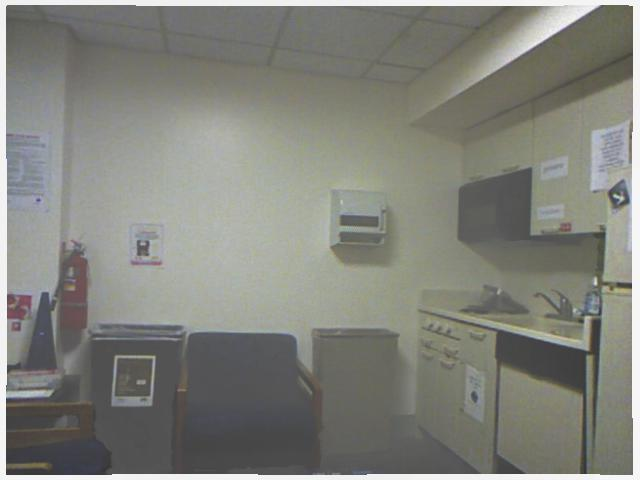
\includegraphics[width=5cm]{hazerd/nyu/dehaze_zhu}}
  \subcaption{}
\end{subfigure}
\hfill
\begin{subfigure}[b]{0.45\linewidth}
  \centering
  \centerline{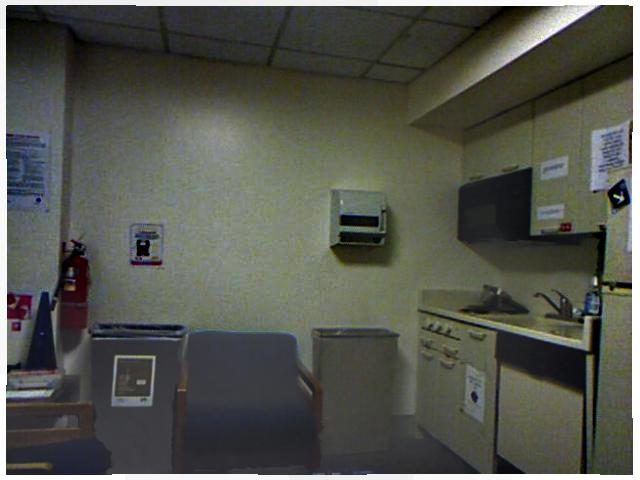
\includegraphics[width=5cm]{hazerd/nyu/dehaze_berman}}
  \subcaption{}
\end{subfigure}
\vfill
\begin{subfigure}[b]{0.45\linewidth}
  \centering
  \centerline{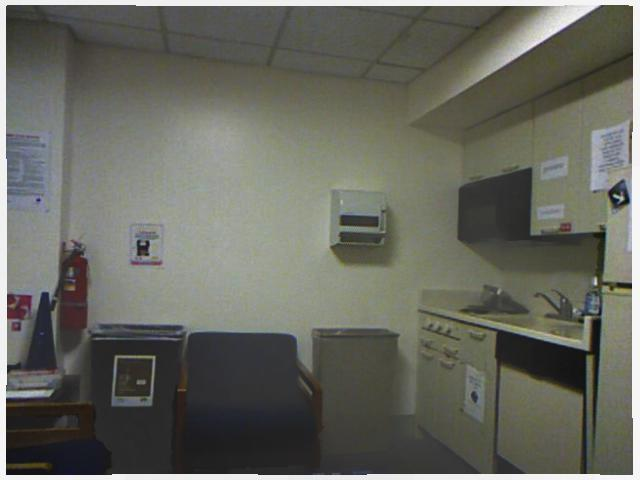
\includegraphics[width=5cm]{hazerd/nyu/dehaze_cai}}
  \subcaption{}
\end{subfigure}
\hfill
\begin{subfigure}[b]{0.45\linewidth}
  \centering
  \centerline{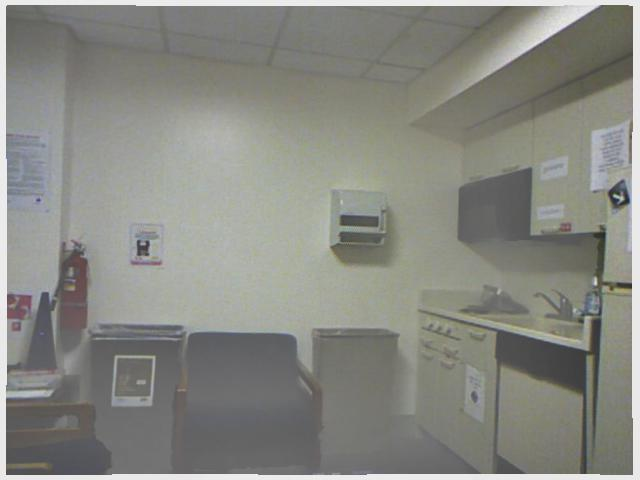
\includegraphics[width=5cm]{hazerd/nyu/dehaze_ren}}
  \subcaption{}
\end{subfigure}
\vfill
\caption{Example of algorithms' performances. (a): a haze free image from NYU dataset, and the results of dehazing of a corresponding hazy image obtained with: (b):He~\cite{he2011single}, (c): Meng~\cite{meng2013efficient}, (d): Zhu~\cite{zhu2015fast}, (e): Berman~\cite{berman2016non}, (f): Cai~\cite{cai2016dehazenet}, and (g): Ren~\cite{Ren-ECCV-2016}.}
\label{fig:3.exmaple.nyu}
\end{figure*}

He~\cite{he2011single} observed that in haze free images, usually the lowest value of a pixel among three channels is close to  zero. Thereby from~\eqref{eq:3.3} in hazy images, the lowest value, called dark channel prior, is an approximation of the transmission. Soft-matting or a guided filter is used as refinement to fit the estimated transmission to the object outlines. This prior is developed further by others, for example into Meng's~\cite{meng2013efficient} color boundary prior and Zhu's~\cite{zhu2015fast} color attenuation prior. The color boundary prior argues that for each image, the color directions are constrained in a cube. The dark channel prior can be derived from the boundary prior with appropriate choice of parameters. The color attenuation prior assumes that the depth can be modeled based on on pixels' saturation and intensity.

Fattal and Berman~\cite{fattal2014dehazing,berman2016non} developed single image dehazing algorithms from the color consistency view, called color-line, or haze-line. In their work, the colors of pixels are assumed to be consistent in a small patch of the object. Given the image formation process, patches of the same color should be co-linear, resulting in the so called color-line, and the shifts indicate the optical distance. The difficulty lies in detecting validated patches and in interpolation for the invalid ones. Haze-line is the clustering of the quantized colors, which avoid the complication of patch detection. 

Besides these algorithms with strong assumptions, deep learning concepts are also exploited in dehazing algorithms. Cai~\cite{cai2016dehazenet} proposed a four-layer network consisting of a CNN layer, a multi-scale mapping layer, a max pooling layer and a fully-connected layer. The training set is formed from synthesized patches with homogeneous transmission. Ren~\cite{Ren-ECCV-2016} proposed a coarse-to-fine network consisting of cascade of CNN layers. The training set is obtained as crops from the NYU dataset. Both methods trained the neural network to compute the transmission.

The performance of dehazing techniques can be evaluated from two perspectives: the accuracy of estimated transmission maps and the fidelity of the dehazed images, each with respect to the corresponding ground truth. We use root mean square (RMS) error to evaluate the difference of the estimated transmission and the ground truth, SSIM~\cite{1284395} to evaluate the similarity of dehazed images and the original haze free images, and CIEDE2000~\cite{sharma2005ciede2000} to evaluate the color fidelity. Results for the algorithms benchmarked and across the different individual datasets are summarized in Table.~\ref{table0}. These results show that typically the transmission values (which are always smaller than 1) have a large error, and the SSIM and CIEDE2000 metrics also show that the dehazed images have significant perceptible difference with the original images. The performance of most of the techniques tested here varies with different weather conditions. Table.~\ref{table0} also lists the weather condition, or equivalently visual range, that yields the best average performance for each algorithm. The tabulated values indicate that algorithms based on priors are limited largely due to the scene and the weather. Generally, these algorithms are not reliable in the sense of dehazing. The visual range for indoor dataset, Middlebury and NYU dataset, is expanded to 5m, 10m, 20m and 50m compared to~\cite{7532754}. Contrasting the differences between indoor and outdoor scenes is important for that generally dehazing techniques are more likely to be used in the latter case. For each algorithm, we run the T-test on the RMS, the SSIM and the CIEDE2000 of HazeRD and the two reference datasets. These datasets shows statistically significant differences between the performances of most algorithms ($\alpha =5\%$). This demonstrates the value of HazeRD as an alternative benchmark for dehazing algorithms: the results on the indoor datasets with limited depth range do not appear to hold for the outdoor datasets.
\begin{landscape}

\begin{table}[htp]
\centering
\vspace*{0.8in}
\resizebox{1.4\textheight}{!}{\begin{tabular}{|c|c|c|c|c|c|c|c|} \hline
\multicolumn{2}{|c|}{} & He~\cite{he2011single} & Meng~\cite{meng2013efficient} & Zhu~\cite{zhu2015fast} & Berman~\cite{berman2016non} & Cai~\cite{cai2016dehazenet} & Ren~\cite{Ren-ECCV-2016} \\
\hline
\multirow{4}{*}{HazeRD} & RMS & 0.2978 $\pm$ 0.0902 & 0.3007 $\pm$ 0.0927 & \textbf{0.1991 $\pm$ 0.0641} & 0.2193 $\pm$ 0.1113 & 0.2765 $\pm$ 0.1002 & 0.2680 $\pm$ 0.0990 \\
\cline{2-8} & SSIM & 0.5148 $\pm$ 0.1293 & 0.6464 $\pm$ 0.1723 & \textbf{0.6692 $\pm$ 0.1979} & 0.5962 $\pm$ 0.1593 & 0.4770 $\pm$ 0.1808 & 0.6664 $\pm$ 0.2013 \\
\cline{2-8}& CIEDE2000 & 20.7038 $\pm$ 4.2821 & 17.2284 $\pm$ 5.0159 & 15.4259 $\pm$ 5.7246 & 19.0647 $\pm$ 4.8029 & 19.5447 $\pm$ 4.8312 & \textbf{14.5432 $\pm$ 6.0696} \\
\cline{2-8}& Best at & dense & thick to light & moderate to light & no preference & dense & light \\ \hline
\multirow{4}{*}{Middlebury} & RMS & 0.2142 $\pm$ 0.1242 & 0.2461 $\pm$ 0.1408 & 0.1921 $\pm$ 0.0985$^*$ & 0.2551 $\pm$ 0.1084$^*$ & \textbf{0.1792 $\pm$ 0.0792} & 0.2022 $\pm$ 0.0980 \\   
\cline{2-8}& SSIM & \textbf{0.7046 $\pm$ 0.1383} & 0.5788 $\pm$ 0.2487 & 0.6394 $\pm$ 0.2524 & 0.6093 $\pm$ 0.2200 & 0.6227 $\pm$ 0.2556 & 0.5978 $\pm$ 0.2522 \\ 
\cline{2-8}& CIEDE2000 & 19.3802 $\pm$ 6.6979 & \textbf{18.4290 $\pm$ 4.7335}$^*$ & 19.8333 $\pm$ 12.2146$^*$ & 19.1038 $\pm$ 6.6742$^*$ & 18.8720 $\pm$ 10.4724$^*$ & 20.0272 $\pm$ 11.1873 \\
\cline{2-8}& Best at & 10m/20m & 50m & 50m & 50m & 20m/50m & 50m\\ \hline
\multirow{4}{*}{NYU} & RMS & 0.2074 $\pm$ 0.1121 & 0.2404 $\pm$ 0.1228 & 0.1998 $\pm$ 0.0845$^*$ & 0.2119 $\pm$ 0.0769$^*$ & \textbf{0.1976 $\pm$ 0.0772} & 0.1995 $\pm$ 0.0758 \\   
\cline{2-8}& SSIM & 0.6478 $\pm$ 0.0518 & \textbf{0.7203 $\pm$ 0.0596} & 0.7029 $\pm$ 0.1668$^*$ & 0.7100 $\pm$ 0.0763 & 0.6773 $\pm$ 0.1261 & 0.7044 $\pm$ 0.1459$^*$ \\ 
\cline{2-8}& CIEDE2000 & 19.7528 $\pm$ 3.6458$^*$ & 16.9486 $\pm$ 2.8969$^*$ & 16.2086 $\pm$ 8.1587$^*$ & 15.7918 $\pm$ 2.8642 & 16.5856 $\pm$ 5.5898 & \textbf{15.4301 $\pm$ 7.3678}$^*$ \\
\cline{2-8}& Best at & 10m & 10m~50m & 50m & 20m/50m & 20m & 50m\\ \hline 
\end{tabular}}
\caption{Performance of different dehazing methods on HazeRD, Middlebury, and NYU datasets. Each numerical entry is represented as the average over the images in the dataset$\pm$the standard deviation. The best performing algorithm for each dataset is indicated in bold font, and * in the Middlebury and NYU datasets indicates cases where the difference with respect to HazeRD was not statistically significant (5\% level).}
\label{table0}
\end{table}
\end{landscape}


The regions in which these algorithms fail on the HazeRD database also provides insight. Algorithms based on dark channel assume all white or bright area is mainly caused by skylight. In HazeRD, there are several white or bright walls which undermine these assumptions, for example, see figure.~\ref{fig:3.scatterhist}. Typical dark channel values are above 0.2, and the error is almost linear in all weather conditions. The haze-line algorithm also has difficulty on bright surfaces, especially rough surfaces. The fluctuations in such surfaces are amplified to a large color difference. Cai's~\cite{cai2016dehazenet} algorithm tends to underestimate the transmission in sky area, which may be caused by the training set, generated by cropping small patches merely from images, and assigning a uniform random depth for each patch.
% \vspace*{-0.0in}
% \begin{table*}[htp]
% \centering
% \resizebox{1\textwidth}{!}{\begin{tabular}{|c|c|c|c|c|c|c|c|} \hline
% \multicolumn{2}{|c|}{} & He~\cite{he2011single} & Meng~\cite{meng2013efficient} & Zhu~\cite{zhu2015fast} & Berman~\cite{berman2016non} & Cai~\cite{cai2016dehazenet} & Ren~\cite{Ren-ECCV-2016} \\
% \hline
% \multirow{4}{*}{HazeRD} & RMS & 0.2028$\pm$0.0866 & 0.1974$\pm$0.0889 & \textbf{0.1459$\pm$0.0490} & 0.2347$\pm$0.0990 & 0.2138$\pm$0.0831 & 0.2411$\pm$0.0974 \\
% \cline{2-8} & SSIM & 0.5457$\pm$0.0083 & 0.6982$\pm$0.0123 & 0.7311$\pm$0.0193 & 0.5491$\pm$0.0144 & 0.4648$\pm$0.0339 & \textbf{0.7897$\pm$0.1329} \\
% \cline{2-8}& CIEDE2000 & 18.7551$\pm$3.5210 & 15.2452$\pm$3.3512 & \textbf{12.4954$\pm$3.0156} & 18.4892$\pm$3.6591 & 17.9828$\pm$4.2385 & 14.0778$\pm$4.1061 \\
% \cline{2-8}& Best at & dense & no preference & thick to light & dense & dense & thick to moderate\\ \hline
% \multirow{4}{*}{Middlebury} & RMS & \textbf{0.1174$\pm$0.0762} & 0.1583$\pm$0.1091* & 0.2157$\pm$0.1072 & 0.2445$\pm$0.0825* & 0.1626$\pm$0.0700 & 0.1664$\pm$0.0629 \\   
% \cline{2-8}& SSIM & \textbf{0.7699$\pm$0.1196} & 0.6502$\pm$0.1852 & 0.6644$\pm$0.2352 & 0.6681$\pm$0.1806 & 0.6613$\pm$0.2345 & 0.6940$\pm$0.2150 \\ 
% \cline{2-8}& CIEDE2000 & \textbf{12.5722$\pm$5.9615} & 15.7742$\pm$5.5110 & 16.1685$\pm$11.2835 & 14.6017$\pm$5.9953 & 15.1969$\pm$9.9048 & 17.2116$\pm$9.2045 \\
% \cline{2-8}& Best at & 20m & 10m/20m & 10m/20m & 10m/20m & 20m & 10m/20m\\ \hline
% \multirow{4}{*}{NYU} & RMS & \textbf{0.1304$\pm$0.0690} & 0.1601$\pm$0.0928 & 0.2172$\pm$0.0952 & 0.1817$\pm$0.0634 & 0.1635$\pm$0.0559 & 0.1744$\pm$0.0554 \\
% \cline{2-8}& SSIM & 0.7750$\pm$0.0606 & \textbf{0.8062$\pm$0.0522*} & 0.7724$\pm$0.1609 & 0.7984$\pm$0.0707 & 0.7918$\pm$0.1312 & 0.7877$\pm$0.1367 \\ 
% \cline{2-8}& CIEDE2000 & 16.2852$\pm$3.8677 & 14.9542$\pm$3.2150 & 13.8445$\pm$7.9453 & 13.1180$\pm$3.3060 & \textbf{12.9625$\pm$5.6995} & 13.0866$\pm$6.6003 \\
% \cline{2-8}& Best at & no preference & no preference & 20m & 10m/20m & 10m/20m & 10m/20m\\ \hline 
% \end{tabular}}
% \vspace*{-0.1in}
% \caption{Performance of different dehazing methods on HazeRD, Middlebury, and NYU datasets. Each numerical entry is represented as the average over the images in the dataset$\pm$the standard deviation. The best performing algorithm for each dataset is indicated in bold font, and * in the Middlebury and NYU datasets indicates cases where the difference with respect to HazeRD was not statistically significant (5\% level).\vspace*{-0.1in}}
% \label{table0}
% \end{table*}
\begin{figure}[ht]
\begin{minipage}[b]{0.45\linewidth}
  \centering
  \centerline{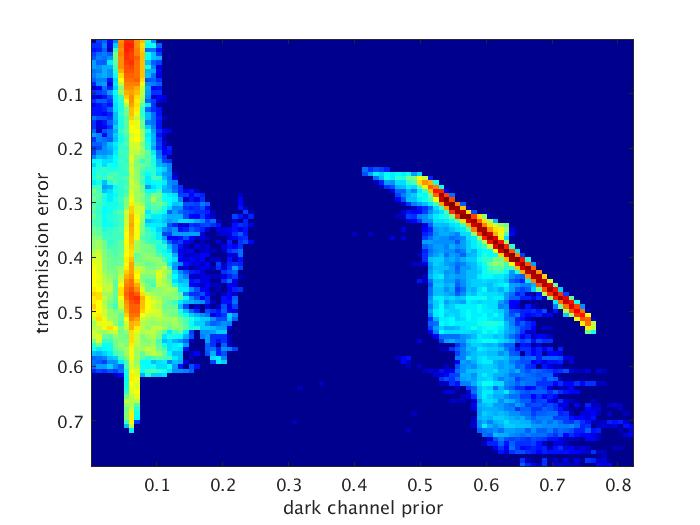
\includegraphics[width=7.5cm]{hazerd/scatterhist/50}}
%  \vspace{1.5cm}
%   \centerline{(a)}\medskip
\end{minipage}
%
\hfill
\begin{minipage}[b]{0.45\linewidth}
  \centering
  \centerline{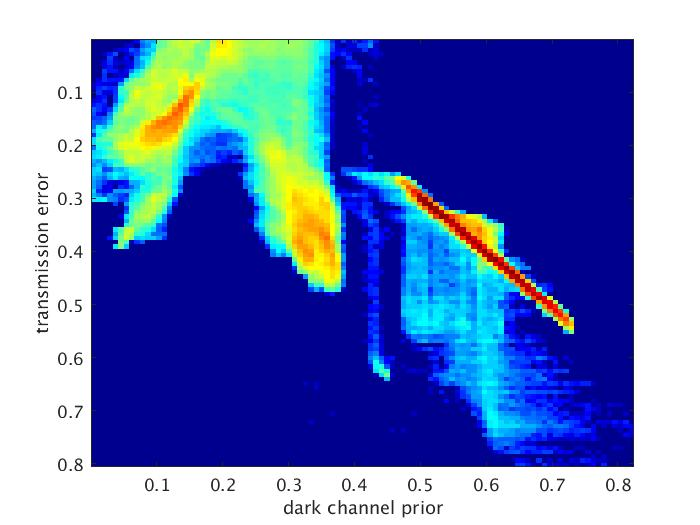
\includegraphics[width=7.5cm]{hazerd/scatterhist/200}}
%  \vspace{1.5cm}
%   \centerline{(b)}\medskip
\end{minipage}
\hfill
\begin{minipage}[b]{0.45\linewidth}
  \centering
  \centerline{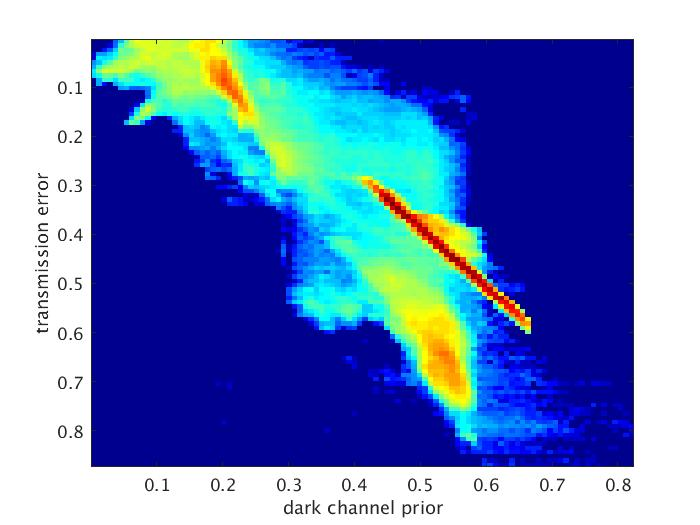
\includegraphics[width=7.5cm]{hazerd/scatterhist/500}}
%  \vspace{1.5cm}
%   \centerline{(c)}\medskip
\end{minipage}
\hfill
\begin{minipage}[b]{0.45\linewidth}
  \centering
  \centerline{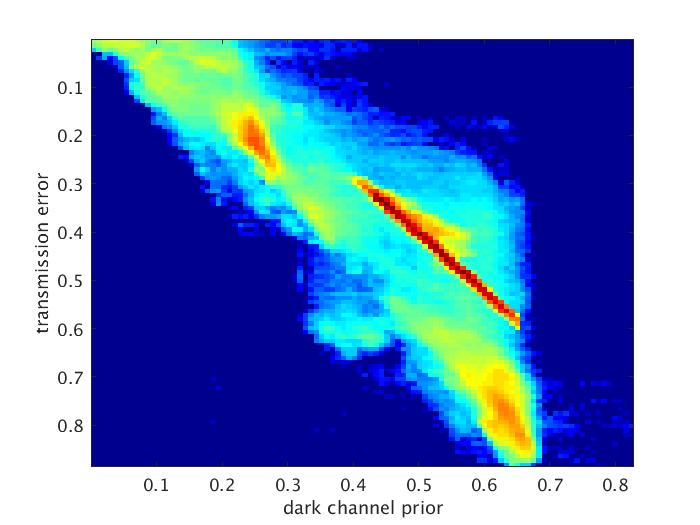
\includegraphics[width=7.5cm]{hazerd/scatterhist/1000}}
%  \vspace{1.5cm}
%   \centerline{(d)}\medskip
\end{minipage}
\caption{Scatter diagram of one scene of the dark channel prior error (y axis) and the transmission error (x axis) in log scale. Each point represents the density of pixels with similar prior-transmission ratios. See the bright line. The dark prior channel is above 0.2 in most area, which is contradictory to the assumption. The transmission error is almost linearly related to the dark channel error. From left to right, fog: dense, thick, moderate, light.}
\label{fig:3.scatterhist}
\end{figure}
\section{discussion}
\label{sec:3.6.discussion}
As we have seen from the experiment results, none of the algorithms benchmarked here provides a sound estimate for the transmission on the HazeRD dataset and each algorithm suffers from some artifacts or color infidelity. In other words, most algorithms seem to focus on enhancing the contrast or saturation without regard to what the true haze free image would be. Partly the reason is that some priors don't hold true on these images. Generally most priors are observations based on particular kinds of images, not the physical model itself. Another easily overlooked problem is that the skylight is not actually uniform but exhibits a gradual variation. In fact, we expect the clear dehazed sky to be blue and not the gray or white that is commonly observed. Last but not least, the performance of most of the techniques tested here varies depending on the weather condition, which indicates that proposed priors should be tested systematically and that training sets for deep learning methods should include more comprehensive situations.

The results we obtained here indicate that indoor and outdoor scenes have some fundamental differences on dehazing techniques and  HazeRD provides a valuable alternative for the benchmarking for dehazing algorithms in more realistic outdoor settings. HazeRD is also a potential dataset for benchmarking of other algorithms including monocular image depth estimation, outdoor scene segmentation, and other applications requiring RGB-D information.